\documentclass[9pt]{beamer}

\usetheme[progressbar=frametitle]{metropolis}
\usepackage[italian]{babel}

\usepackage{paralist}

\usepackage{appendixnumberbeamer}

\usepackage{amsmath}

\usepackage{booktabs}
\usepackage[scale=2]{ccicons}

\usepackage{pgfplots}
\usepgfplotslibrary{dateplot}

\usepackage{xspace}
\newcommand{\themename}{\textbf{\textsc{metropolis}}\xspace}

\title{TSP con pick up and delivery}
\subtitle{Progetto del corso di Ricerca Operativa}
\date{1 febbraio 2023}
\author{Michele Vaccari - Matricola 121955}
\institute{Università degli studi di Ferrara\\Corso di laurea magistrale in Ingegneria Informatica e dell'Automazione\\AA 2020-2021}

% logo of my university
\titlegraphic{%
  \begin{picture}(0,0)
    \put(305,0){\makebox(0,0)[rt]{
\includegraphics[width=4cm]{../images/logo-unife}}}
  \end{picture}}

\usepackage{minted}
\usepackage{multicol}
\usepackage{multirow}
\usepackage{adjustbox}
\usepackage{graphicx}
\usepackage{caption}

\begin{document}

\maketitle

%\begin{frame}[allowframebreaks]{Indice}
%  \setbeamertemplate{section in toc}[sections numbered]
%  \tableofcontents
%\end{frame}

%%%
%%%   INTRODUZIONE
%%%

\section{Introduzione}

\subsection{Descrizione del problema}
\begin{frame}{\subsecname}

	\metroset{block=fill}
	\begin{block}{Progettino 24 - TSP con pick up and delivery (1 persona)}
		A partire dalla base (nodo $0$ del grafo) un corriere deve soddisfare $n$ richieste di prelievo e consegna di documenti:
		\begin{compactitem}
			\item 	ogni documento è prelevato in un nodo e consegnato in un altro nodo;
			\item ogni nodo è riferito a una singola richiesta, ma nel tragitto tra punto di prelievo e consegna si possono prelevare/consegnare altri documenti.
		\end{compactitem}
		Noto il tempo di percorrenza dei singoli archi, si vuole minimizzare la durata del percorso, con partenza e rientro al deposito.
	\end{block}

\end{frame}

\subsection{Un esempio di istanza}
\begin{frame}{\subsecname}

	\begin{figure}[h]
		\centering
		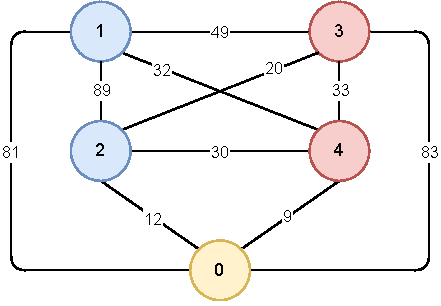
\includegraphics[width=0.6\textwidth]
		{../images/graph-tsppd-with-two-customers}	
		\caption{Istanza con 2 richieste di prelievo e consegna}
	\end{figure}

\end{frame}

\section{Modello matematico per S-TSPPD}
\subsection{Notazione}
\begin{frame}[allowframebreaks]{\subsecname}
	\begin{itemize}
		\item
		Numero di richieste di prelievo e consegna: $n$
		
		\item
		Nodi di pickup: $V_P = \{1, \dots, n\}$
		
		\item
		Nodi di delivery: $V_D = \{n+1, \dots, 2n\}$
		
		\item
		Una richiesta è identificata con la coppia di nodi $(i,n+i)$ e $i$ deve precedere $n+i$ in un percorso ammissibile
		
		\item
		$V$ è definito come l'unione di $V_P$ e $V_D$ con l'aggiunta del nodo di deposito $\{0\}$
		
		\item
		$E_{PD}$ è l'insieme degli archi che connettono $V_P \cup V_D$
	
		\item
		$E$ è l'unione di $E_{PD}$ con tutti gli archi ammissibili che collegano il nodo di deposito
		
		\item
		Il grafo $G=(V,E)$ comprende tutti i nodi e gli archi necessari per descrivere il S-TSPPD (il grafo è completo)
		\[ V=\{0\} \cup V_P \cup V_D \]
		\[ E = \{ (0,i) | i \in V_P \} \cup \{ (0,i) | i \in V_D \} \cup E_{PD} \]
		
		L'insieme degli archi $E$ è definito in modo tale da includere solo archi ammissibili.
		In altre parole, non è possibile che un percorso TSPPD inizi con una consegna o finisca con un prelievo.
		
		\item
		Ogni arco $(i,j) \in E$ è uguale all'arco $(j, i)$

		\item
		Ogni arco ha gli stessi costi e variabili

		\item
		$c_{ij}$ è un costo non negativo per ogni arco $(i,j) \in E$

		\item
		$x_{ij} \in \{ 0, 1 \}$ è una variabile decisionale binaria per ogni $(i, j) \in E$ con il valore $x_{ij} = 1$ se l'arco $(i, j)$ è in una soluzione e $0$ altrimenti

		\item
		$\delta(S) = \{ (i, j) \in E | i \in S, j \notin S$ è il taglio contenente gli archi che collegano $S \subset V$ e $S^* \subset V$ 

		\item
		Per qualsiasi nodo $i \in V, \delta(i) = \delta( \{ i \})$
	\end{itemize}
\end{frame}

\subsection{Modello matematico}
\begin{frame}{\subsecname}

     	\[ min{ \sum_{(i,j) \in E} c_i x_{ij}} \]
	tale che
	\begin{enumerate}
		\item
		\label{stsppd-c1}
		$x_0 = 1$

		\item
		\label{stsppd-c2}
		$x(\delta(i)) = 2 \quad \forall i \in V$

		\item
		\label{stsppd-c3}
		$x(\delta(i)) \geq 2 \quad \forall S \subset V$
	
		\item
		\label{stsppd-c4}
		$x(\delta(i)) \geq 4 \quad \forall S \subset V, \{0, n+i\} \subset S, \{0,i\} \subset V \setminus S$	% TODO: Fix this costraint

		\item
		$x_{ij} \in \{0,1\} \quad (i,j) \in E$
	\end{enumerate}
	
	\footnotesize
	Il vincolo \ref{stsppd-c1} richiede che l'arco che collega il nodo di deposito faccia parte di qualsiasi soluzione ammissibile. \\
	Il vincolo \ref{stsppd-c2} richiede che ogni nodo entri ed esca in tutti i percorsi ammissibili, ma di per sé lascia aperta la possibilità di sotto-tour, formando una rappresentazione completa del TSP. \\
	Il vincolo \ref{stsppd-c3} consente di eliminare i sotto-tour, formando una rappresentazione completa del TSP. \\
	Il vincolo \ref{stsppd-c4} richiede che i ritiri avvengano prima delle rispettive consegne

\end{frame}

\section{Modello matematico per A-TSPPD}
\subsection{Notazione}
\begin{frame}[allowframebreaks]{\subsecname}
	\begin{itemize}
		\item
		Numero di richieste di prelievo e consegna: $n$
		
		\item
		Nodi di pickup: $N_P = \{1, \dots, n\}$
		
		\item
		Nodi di delivery: $N_D = \{n+1, \dots, 2n\}$
		
		\item
		Una richiesta è identificata con la coppia di nodi $(i,n+i)$ e $i$ deve precedere $n+i$ in un percorso ammissibile
		
		\item
		$N$ è definito come l'unione di $N_P$ e $N_D$ con l'aggiunta del nodo di deposito $\{0\}$
		
		\item
		$A_{PD}$ è l'insieme degli archi \emph{orientati} che connettono $N_P \cup N_D$
	
		\item
		$A$ è l'unione di $A_{PD}$ con tutti gli archi \emph{orientati} ammissibili che collegano il nodo di deposito
		
		\item
		Il grafo $G=(N,A)$ comprende tutti i nodi e gli archi necessari per descrivere il A-TSPPD (il grafo è completo)
		\begin{equation*}
			\begin{aligned}
			N= & \{0\} \cup N_P \cup N_D \\
			A = & \{ (0,i) | i \in N_P \} \\
			& \cup \{ (i,0) | i \in N_D \} \\
			& \cup \{ (i,j) | i \in N_P , j \in ( N_P \cup N_D ) \setminus \{ i \} \} \\
			& \cup \{ ( n + i, j) | i \in N_P , j \in (N_P \cup N_D ) \setminus \{ i , n + i \} \}
			\end{aligned}
		\end{equation*}
		
		L'insieme degli archi $A$ è definito in modo tale da includere solo archi ammissibili.
		In altre parole, non è possibile che un percorso TSPPD inizi con una consegna o finisca con un prelievo.

		\item
		$c_{ij}$ è un costo non negativo per ogni arco $(i,j) \in A$

		\item
		$x_{ij} \in \{ 0, 1 \}$ è una variabile decisionale binaria per ogni $(i, j) \in A$ con il valore $x_{ij} = 1$ se l'arco $(i, j)$ è in una soluzione e $0$ altrimenti

		\item
		$\delta(S) = \{ (i, j) \in A | i \in S, j \notin S$ è il taglio contenente gli archi che collegano $S \subset N$ e $S^* \subset N$ 

		\item
		Per qualsiasi nodo $i \in N, \delta(i) = \delta( \{ i \})$
	\end{itemize}
\end{frame}

\subsection{Modello matematico}
\begin{frame}{\subsecname}

     	\[ min{ \sum_{(i,j) \in A} c_i x_{ij}} \]
	tale che
	\begin{enumerate}
		\item
		\label{atsppd-c1}
		$\sum_{(i,j) \in A} x_{ij} = 1 \quad \forall i \in N$

		\item
		\label{atsppd-c2}
		$\sum_{(i,j) \in A} x_{ij} = 1 \quad \forall j \in N$

		\item
		\label{atsppd-c3}
		$x(\delta(S)) \geq 1 \quad \forall S \subset N$
	
		\item
		\label{atsppd-c4}
		$x(\delta(i)) \geq 4 \quad \forall S \subset N, \{0, n+i\} \subset S, \{0,i\} \subset N \setminus S$ 	% TODO: Fix this costraint!!!

		\item
		$x_{ij} \in \{0,1\} \quad (i,j) \in A$
	\end{enumerate}
	
	\footnotesize
	I vincoli \ref{atsppd-c1} e \ref{atsppd-c2} richiedono che ogni nodo preceda e segua direttamente un altro nodo. \\
	Il vincolo \ref{atsppd-c3} consente di eliminare i sotto-tour, formando una rappresentazione completa del TSP. \\
	Il vincolo \ref{atsppd-c4} richiede che i ritiri avvengano prima delle rispettive consegne (è uguale al vincolo \ref{stsppd-c4} del S-TSPPD)

\end{frame}

\begin{frame}{Alcune considerazioni sul problema}
	
	\begin{itemize}
	
		\item
		Di fatto il TSPPD è un TSP con in più i vincoli di precedenza.

		\item
		Sia S-TSPPD che A-TSPPD sono formulazioni che pongono dei problemi per il gran numero di vincoli

		\item
		Un'istanza S-TSP con $n$ coppie ha \( \#TSP = \frac{1}{2} (2n -1)!\) soluzioni distinte \cite{lin1965computer}, mentre un TSPPD della stessa dimensione ha \(\#TSPPD(n) = \frac{2n!}{2^n}\) \cite{ruland1997pickup}
		
		\item
		La dimensione dell'insieme ammissibile del TSPPD cresce più lentamente rispetto al numero di coppie di nodi rispetto a quella del TSP

		\item
		Ovviamente, l'insieme delle soluzioni ammissibili del TSPPD è un sottoinsieme delle soluzioni fattibili del TSP
		
		\item
		Se si ammettono solo coppie di nodi di ritiro e consegna nel percorso con relazioni di precedenza, la dimensione dell'insieme fattibile del TSP si riduce di \( \frac{1}{2^{n-1}!} \) \cite{ruland1997pickup}
	\end{itemize}

\end{frame}

\subsection{Soluzioni ammissibili per l'istanza d'esempio}
\begin{frame}{\subsecname}

	\begin{figure}[h]
		\centering
		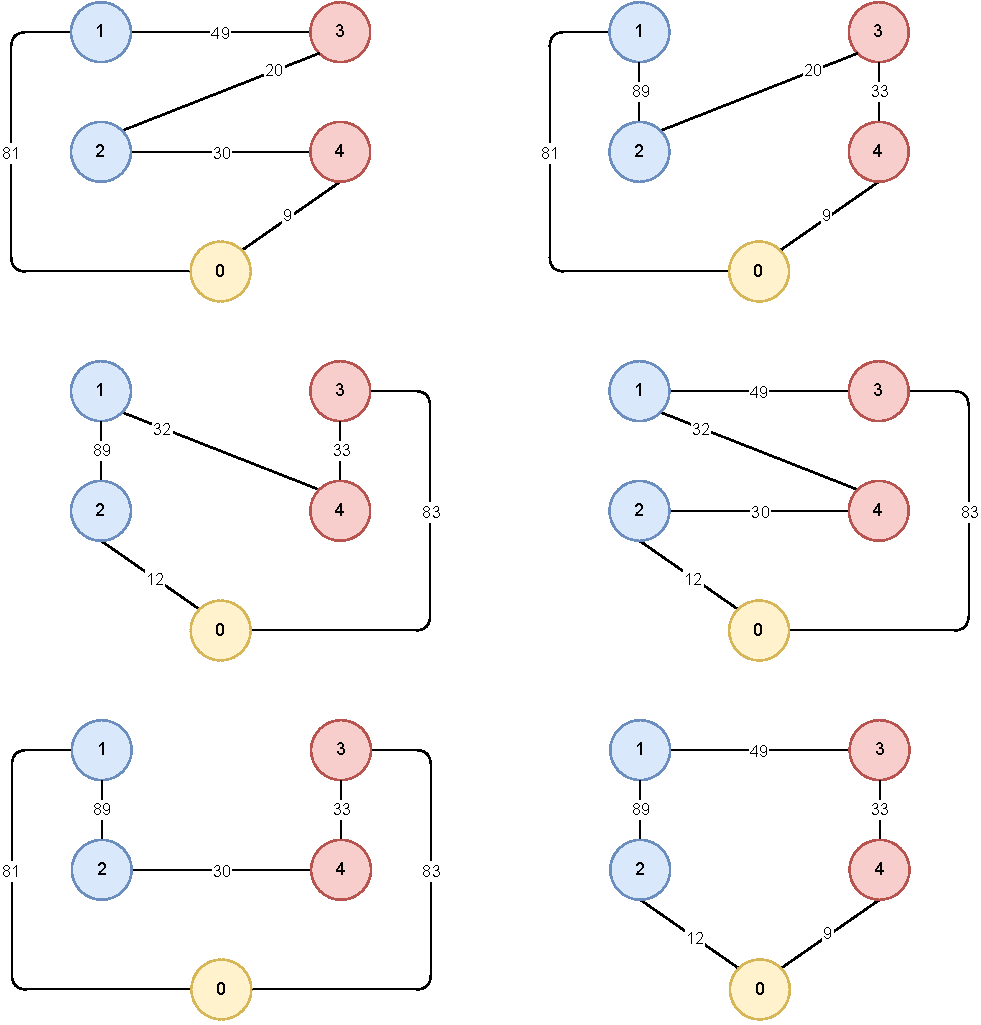
\includegraphics[width=0.6\textwidth]
		{../images/graph-all-solutions-tsppd-with-two-customers}	
		\caption{Soluzioni ammissibili per l'istanza con 2 richieste di prelievo e consegna}
	\end{figure}

\end{frame}

\section{Progetto}

\subsection{Panoramica}
\begin{frame}[allowframebreaks]{\subsecname}

	\textbf{Strumenti utilizzati}
	\begin{itemize}
		\item
		Linguaggio Python 3.10 con le seguenti librerie:
		\begin{itemize}
			\item
			Click
			\item
			Numpy
			\item
			Pytest
			\item
			Openpyxl
			\item
			Stopwatch
		\end{itemize}
		\item
		Visual Studio Code come editor di testo
		\item
		Git per il versionamento del codice
	\end{itemize}

\framebreak

	\textbf{Arichitettura} \\
	L’applicazione è formata da 3 componenti:
	\begin{itemize}
		\item
		\textbf{problem:} è il package che contiene le entità utilizzate per modellare il problema e un generatore di istanze casuali
		\item
		\textbf{solver:} è il package che contiene gli algoritmi implementati. Utilizza le entità definite nel package problem
		\item
		\textbf{cli:} è una Command Line Interface che consente di generare istanze del problema e testare i vari algoritmi
	\end{itemize}

	\textbf{Repository GitHub} \href{https://github.com/michele-vaccari/TSP-con-pick-up-and-delivery}{https://github.com/michele-vaccari/TSP-con-pick-up-and-delivery}

\end{frame}

\subsection{Benchmark}
\begin{frame}{\subsecname}

	\textbf{Automazione} \\
	L'esecuzione e la raccolta dei dati durante i benchmark è stata automatizzata sempre utilizzando il linguaggio Python. Si è utilizzata la libreria Openpyxl in modo tale che i dati vengano collezionati in modo ordinato su fogli di calcolo.

	\textbf{Esecuzione} \\
	I benchmark sono stati eseguiti su un PC con:
	\begin{itemize}
		\item
		\textbf{Sistema operativo:} Windows 10
		\item
		\textbf{Processore:} Intel Core i5-4570 CPU  3.20 GHz
		\item
		\textbf{RAM:} 16.0 GB
	\end{itemize}
	Il tempo di esecuzione complessivo dei benchmark è stato di circa $10$ giorni. Nel dettaglio: $346399.9\;secondi \rightarrow 5773.332\;minuti \rightarrow 240.5555\;ore \rightarrow 10.02315\;giorni$

\end{frame}

\subsection{Generatore di istanze}
\begin{frame}[fragile]{\subsecname}

	È possible generare un istanza del problema nel seguente modo:
	\begin{itemize}
		\item
		\textbf{Istanza asimmetrica} \\
		\mintinline[breaklines]{bash}{python tsppdcli.py generate-instance --requests 2 --weights-random --output-instance-path 2-request-weights-random.jsonn}
		\item
		\textbf{Istanza simmestrica} \\
		\mintinline[breaklines]{bash}{python tsppdcli.py generate-instance --requests 2 --weights-as-euclidean-distance --output-instance-path 2-request-weights-euclidean-distance.json}
	\end{itemize}

	\textbf{Esempio di istanza} \\
	\href{https://github.com/michele-vaccari/TSP-con-pick-up-and-delivery/blob/main/src/instances/2-request.json}{https://github.com/michele-vaccari/TSP-con-pick-up-and-delivery/blob/main/src/instances/2-request.json}

\end{frame}

%%%
%%%   ALGORITMI ESATTI
%%%

\section{Algoritmi esatti}

\subsection{Brute force enumerator}
\begin{frame}[allowframebreaks]{\subsecname}

	\textbf{Descrizione dell’algoritmo} \\
	Vediamo il codice dell’algoritmo Brute force enumerator:
	\href{https://github.com/michele-vaccari/TSP-con-pick-up-and-delivery/blob/main/src/tsppd/solver/bruteForceEnumerator.py}{https://github.com/michele-vaccari/TSP-con-pick-up-and-delivery/blob/main/src/tsppd/solver/bruteForceEnumerator.py}

	\textbf{Esempio}
	\begin{figure}[h]
	\centering
	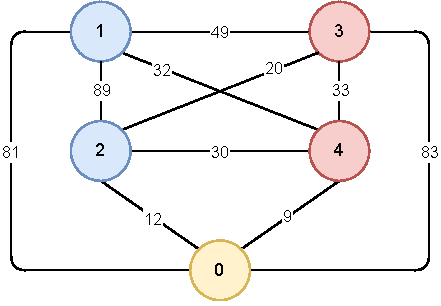
\includegraphics[width=0.4\textwidth]
	{../images/graph-tsppd-with-two-customers}	
	\caption{Istanza iniziale}
	\end{figure}

\framebreak

	\textbf{Esecuzione}
      	\begin{figure}[h]
	\centering
	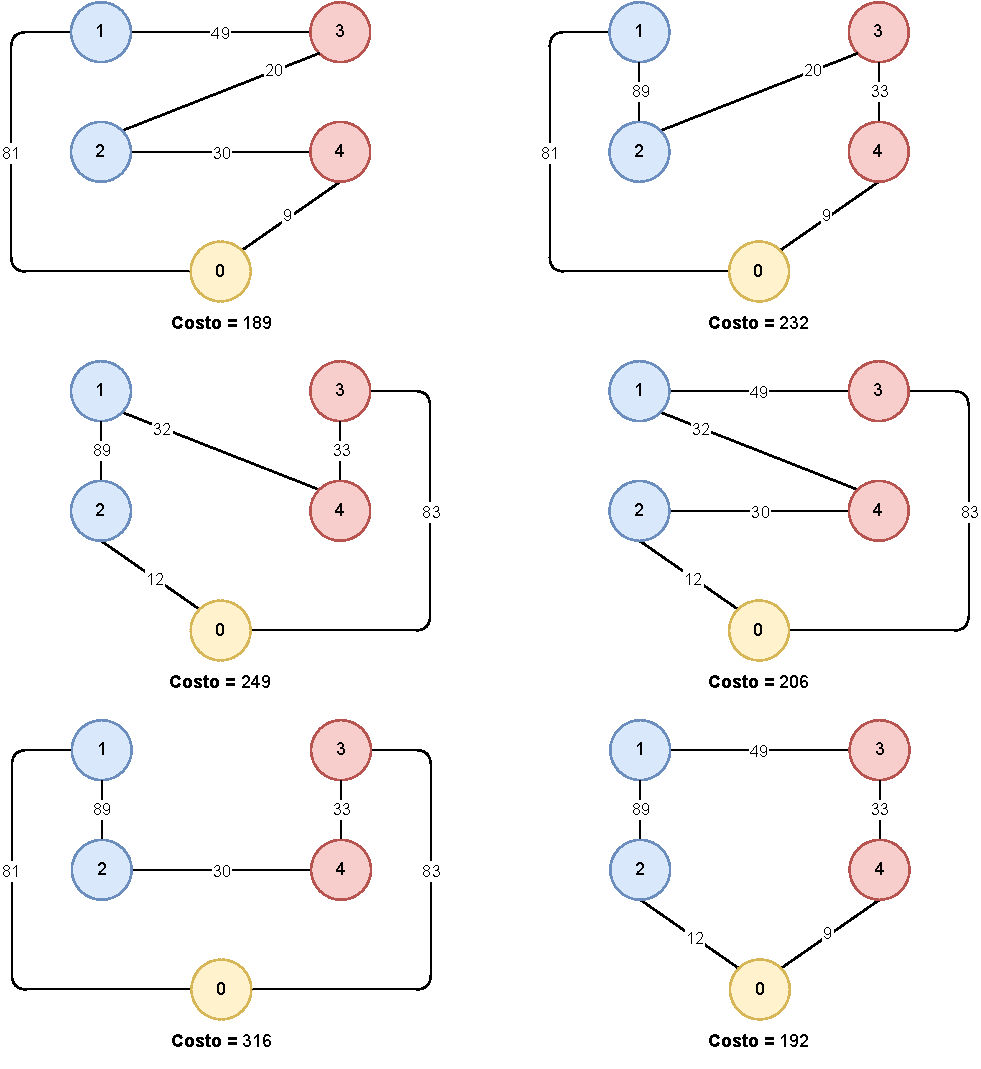
\includegraphics[width=0.45\textwidth]
	{../images/graph-all-solutions-with-cost-tsppd-with-two-customers}	
	\caption{Soluzioni esplorate}
	\end{figure}

\framebreak

	\textbf{Performance nel tempo}
      	\begin{figure}[h]
	\centering
	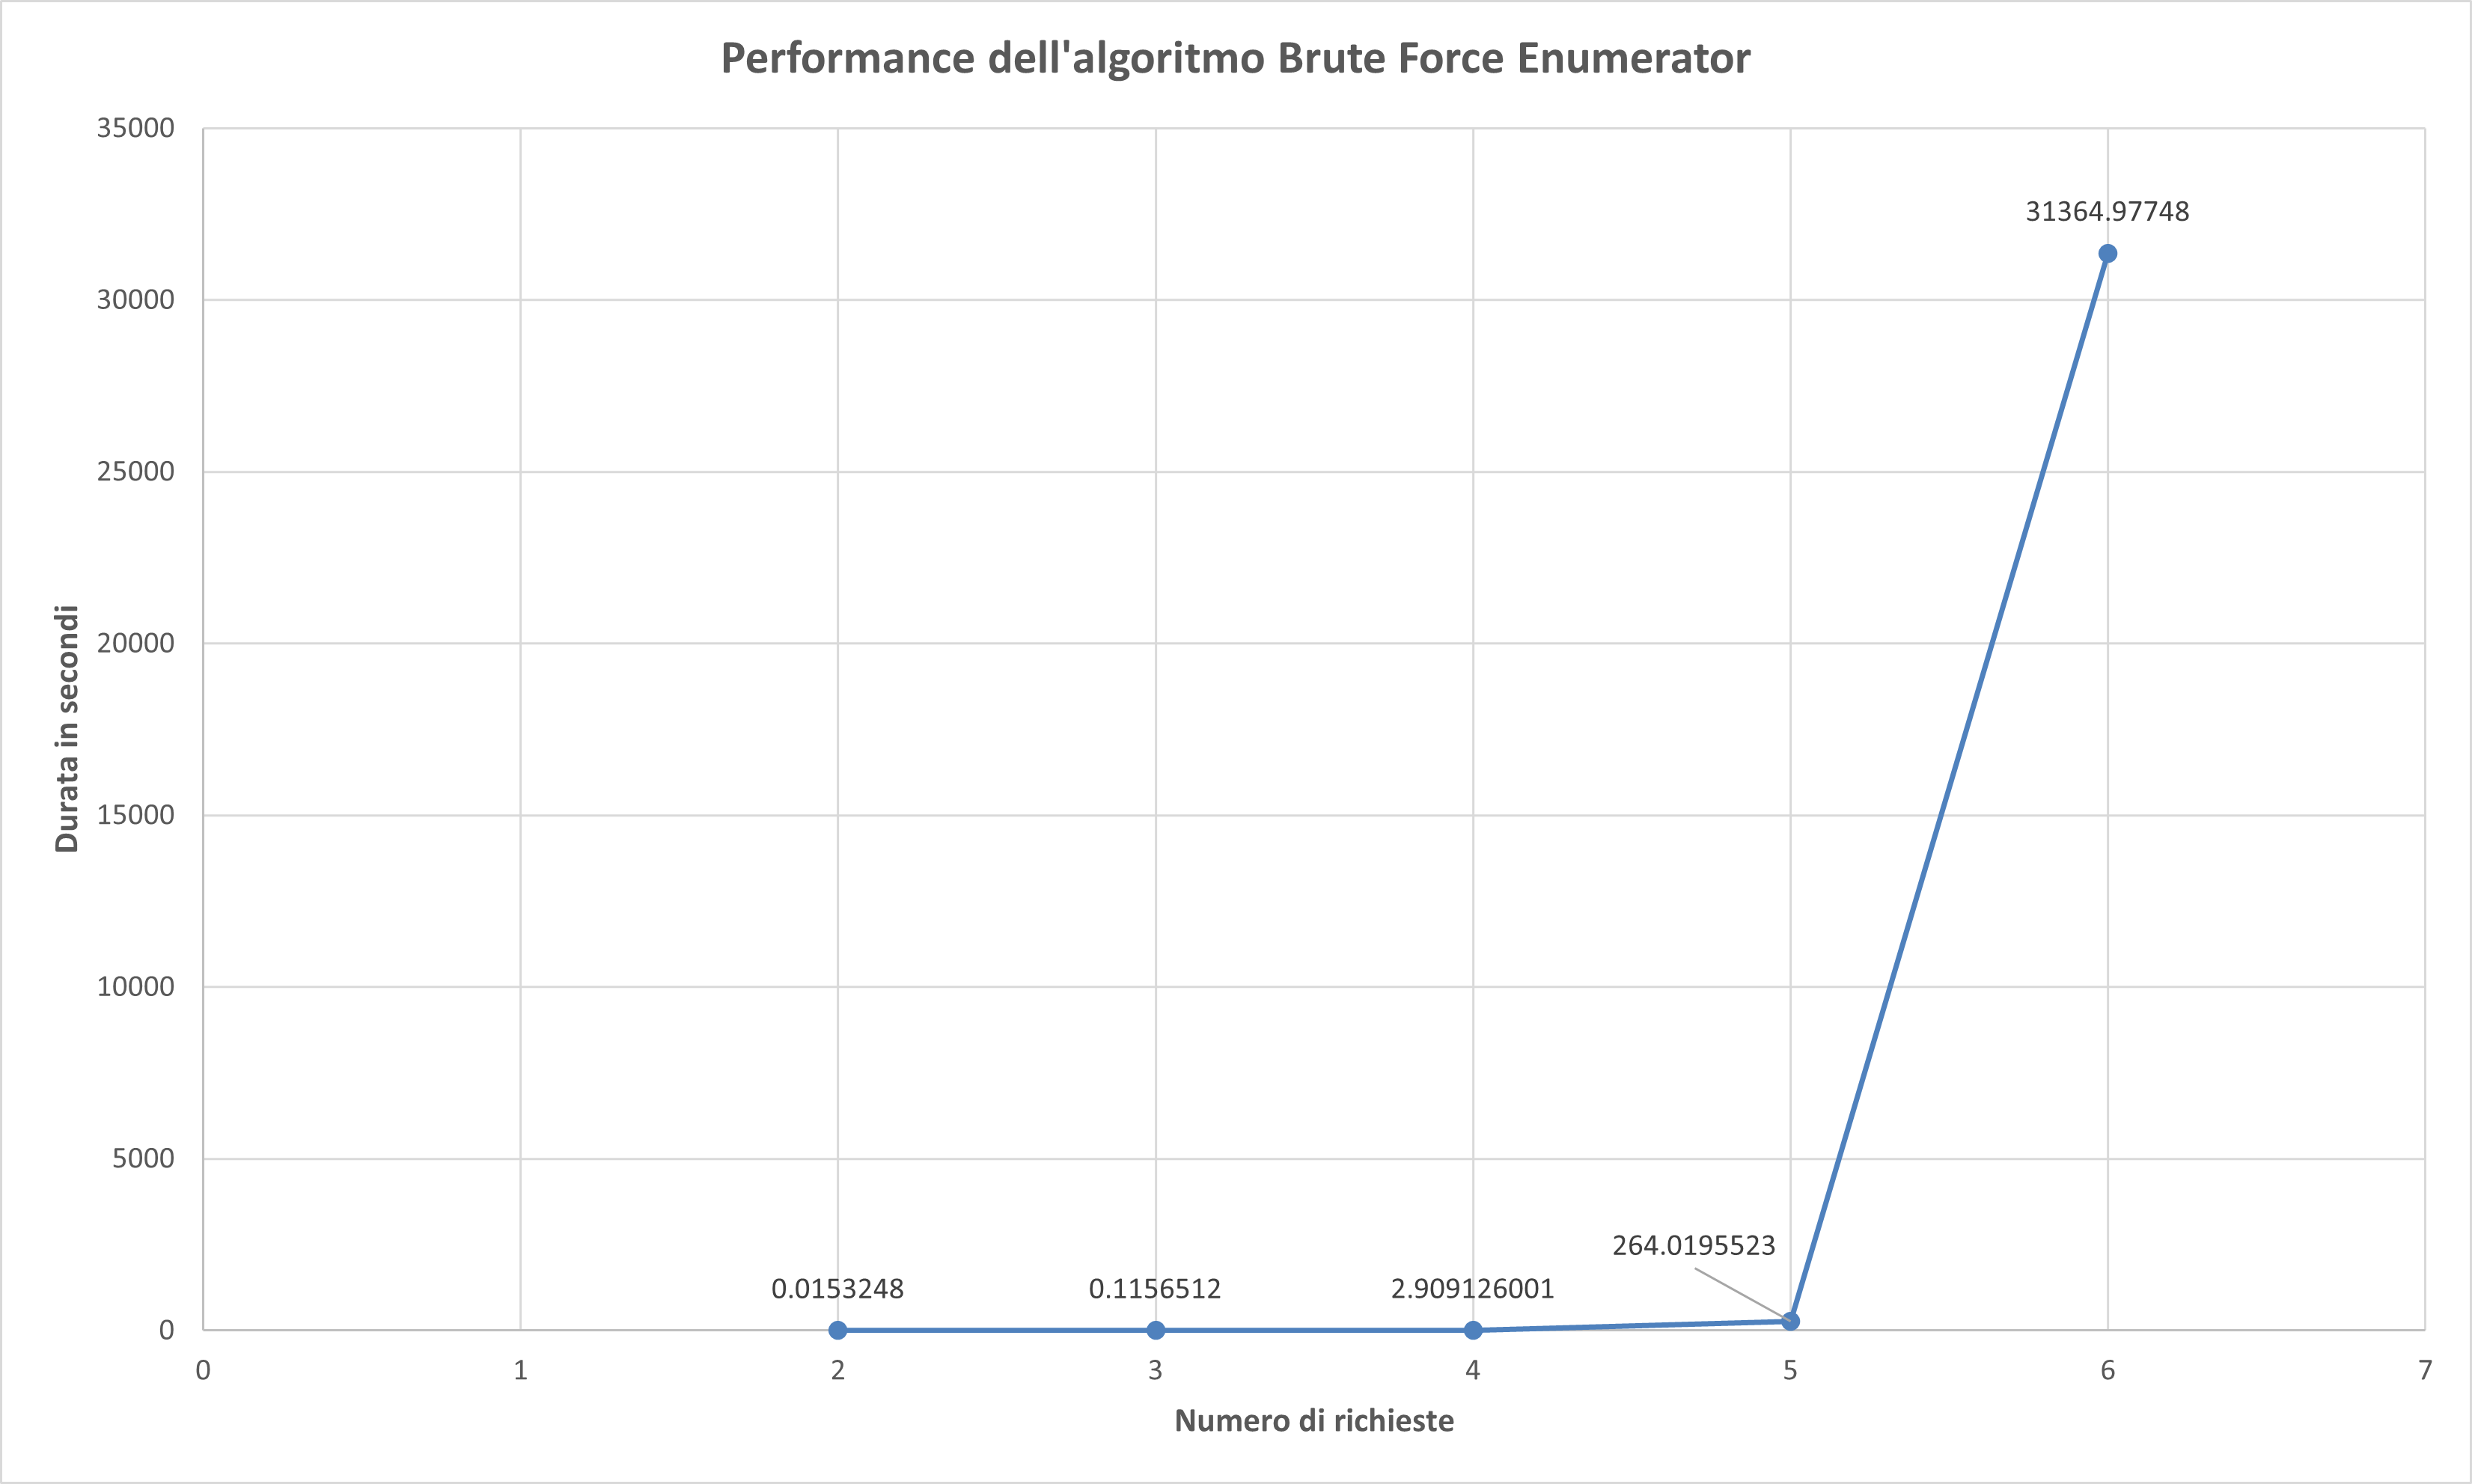
\includegraphics[width=\textwidth]
	{../charts/01 Performance dell'algoritmo Brute Force Enumerator}
	\end{figure}

\end{frame}

\subsection{O’Neil -- Hoffman enumerator}
\begin{frame}[allowframebreaks, fragile]{\subsecname}

	\begin{columns}[T,onlytextwidth]
		\column{0.5\textwidth}
		\begin{minted}[fontsize=\tiny, escapeinside=;;, tabsize=2]{c}
function Initialize()
	for all ;$i \in nodes$; do
		;$arcs(i) \leftarrow ordered \{j | j \in nodes \setminus \{ 0 \} , j \neq i\}$;
	;$tour \leftarrow (0)$;
	;$best \leftarrow \emptyset$;

function Enumerate()
	;$n_1 \leftarrow last\,node\,in\,tour$;
	for all ;$n_2 \in arcs(current)$; do
		if ;$n_2 \in tour$;
			continue
		else if ;$cost(tour) + cost(n_1, n_2) \geq cost(best)$;
			continue
		else if ;$n_2 \in N_D$; and ;$pickup(n_2) \notin tour$;
			continue

	;$tour \leftarrow tour + next$;
	if ;$|tour| \geq n - 1$; then
		;$c \leftarrow cost(tour) + cost(n_2, 0)$;
		if ;$best = \emptyset$; or ;$c < cost(best)$;
			;$best \leftarrow tour + 0$;
	else
		Enumerate()

	;$tour \leftarrow tour - next$;

Initialize()
Enumerate()
		\end{minted}
		\column{0.5\textwidth}
		
		{\scriptsize
		\textbf{Descrizione dell’algoritmo} \\

		L'algoritmo O’Neil -- Hoffman \cite{o2018exact} utilizza una funzione ricorsiva per cercare l'insieme ammissibile dei percorsi TSPPD, tenendo traccia della migliore soluzione scoperta in ogni punto dell'albero di ricerca.

		L'algoritmo mantiene un nodo corrente e un percorso parziale che inizia con $0$ (nodo deposito).

		Ogni ricorsione ripercorre gli archi a partire dal nodo corrente e aggiunge ogni arco ammissibile al tour individualmente prima della ricorsione. Se il costo aggiunto da un arco fa sì che il costo di un percorso parziale sia superiore a quello del tour migliore conosciuto, quell'arco viene ignorato e la sua sezione dell'albero di ricerca viene effettivamente esplorata. Se un percorso completo migliora la soluzione migliore conosciuta, viene memorizzato come nuovo ottimo candidato.

		La chiave della ricerca efficace e della scoperta precoce di buone soluzioni è la tecnica di ordinamento degli archi. Durante l'inizializzazione, ad ogni nodo viene assegnato un vettore ordinato di nodi successivi. Come funzione di ordinamento utilizziamo il costo ascendente dell'arco, ma altri possono essere facilmente incorporati.

		I nodi che non sono fattibili per il percorso parziale corrente vengono saltati.

		}
	
	  \end{columns}

\framebreak

	\textbf{Codice} \\
	\href{https://github.com/michele-vaccari/TSP-con-pick-up-and-delivery/blob/main/src/tsppd/solver/oneilHoffmanEnumerator.py}{https://github.com/michele-vaccari/TSP-con-pick-up-and-delivery/blob/main/src/tsppd/solver/oneilHoffmanEnumerator.py}

	\textbf{Esempio}
	\begin{figure}[h]
	\centering
	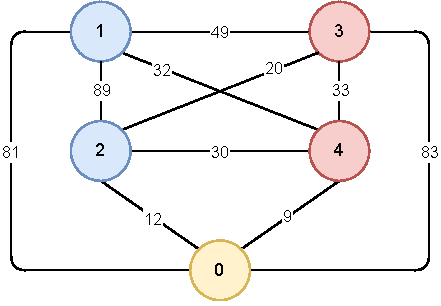
\includegraphics[width=0.5\textwidth]
	{../images/graph-tsppd-with-two-customers}	
	\caption{Istanza iniziale}
	\end{figure}

	\textbf{Esecuzione}
      	\begin{figure}[h]
	\centering
	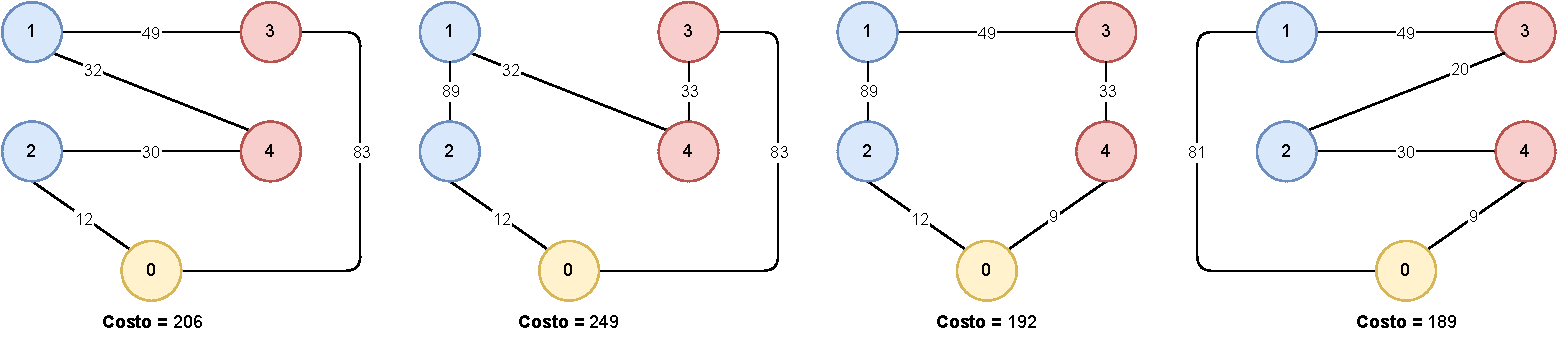
\includegraphics[width=\textwidth]
	{../images/graph-oneil-hoffman-solutions-tsppd-with-two-customers}	
	\caption{Soluzioni esplorate}
	\end{figure}

\framebreak

	\textbf{Performance nel tempo}
      	\begin{figure}[h]
	\centering
	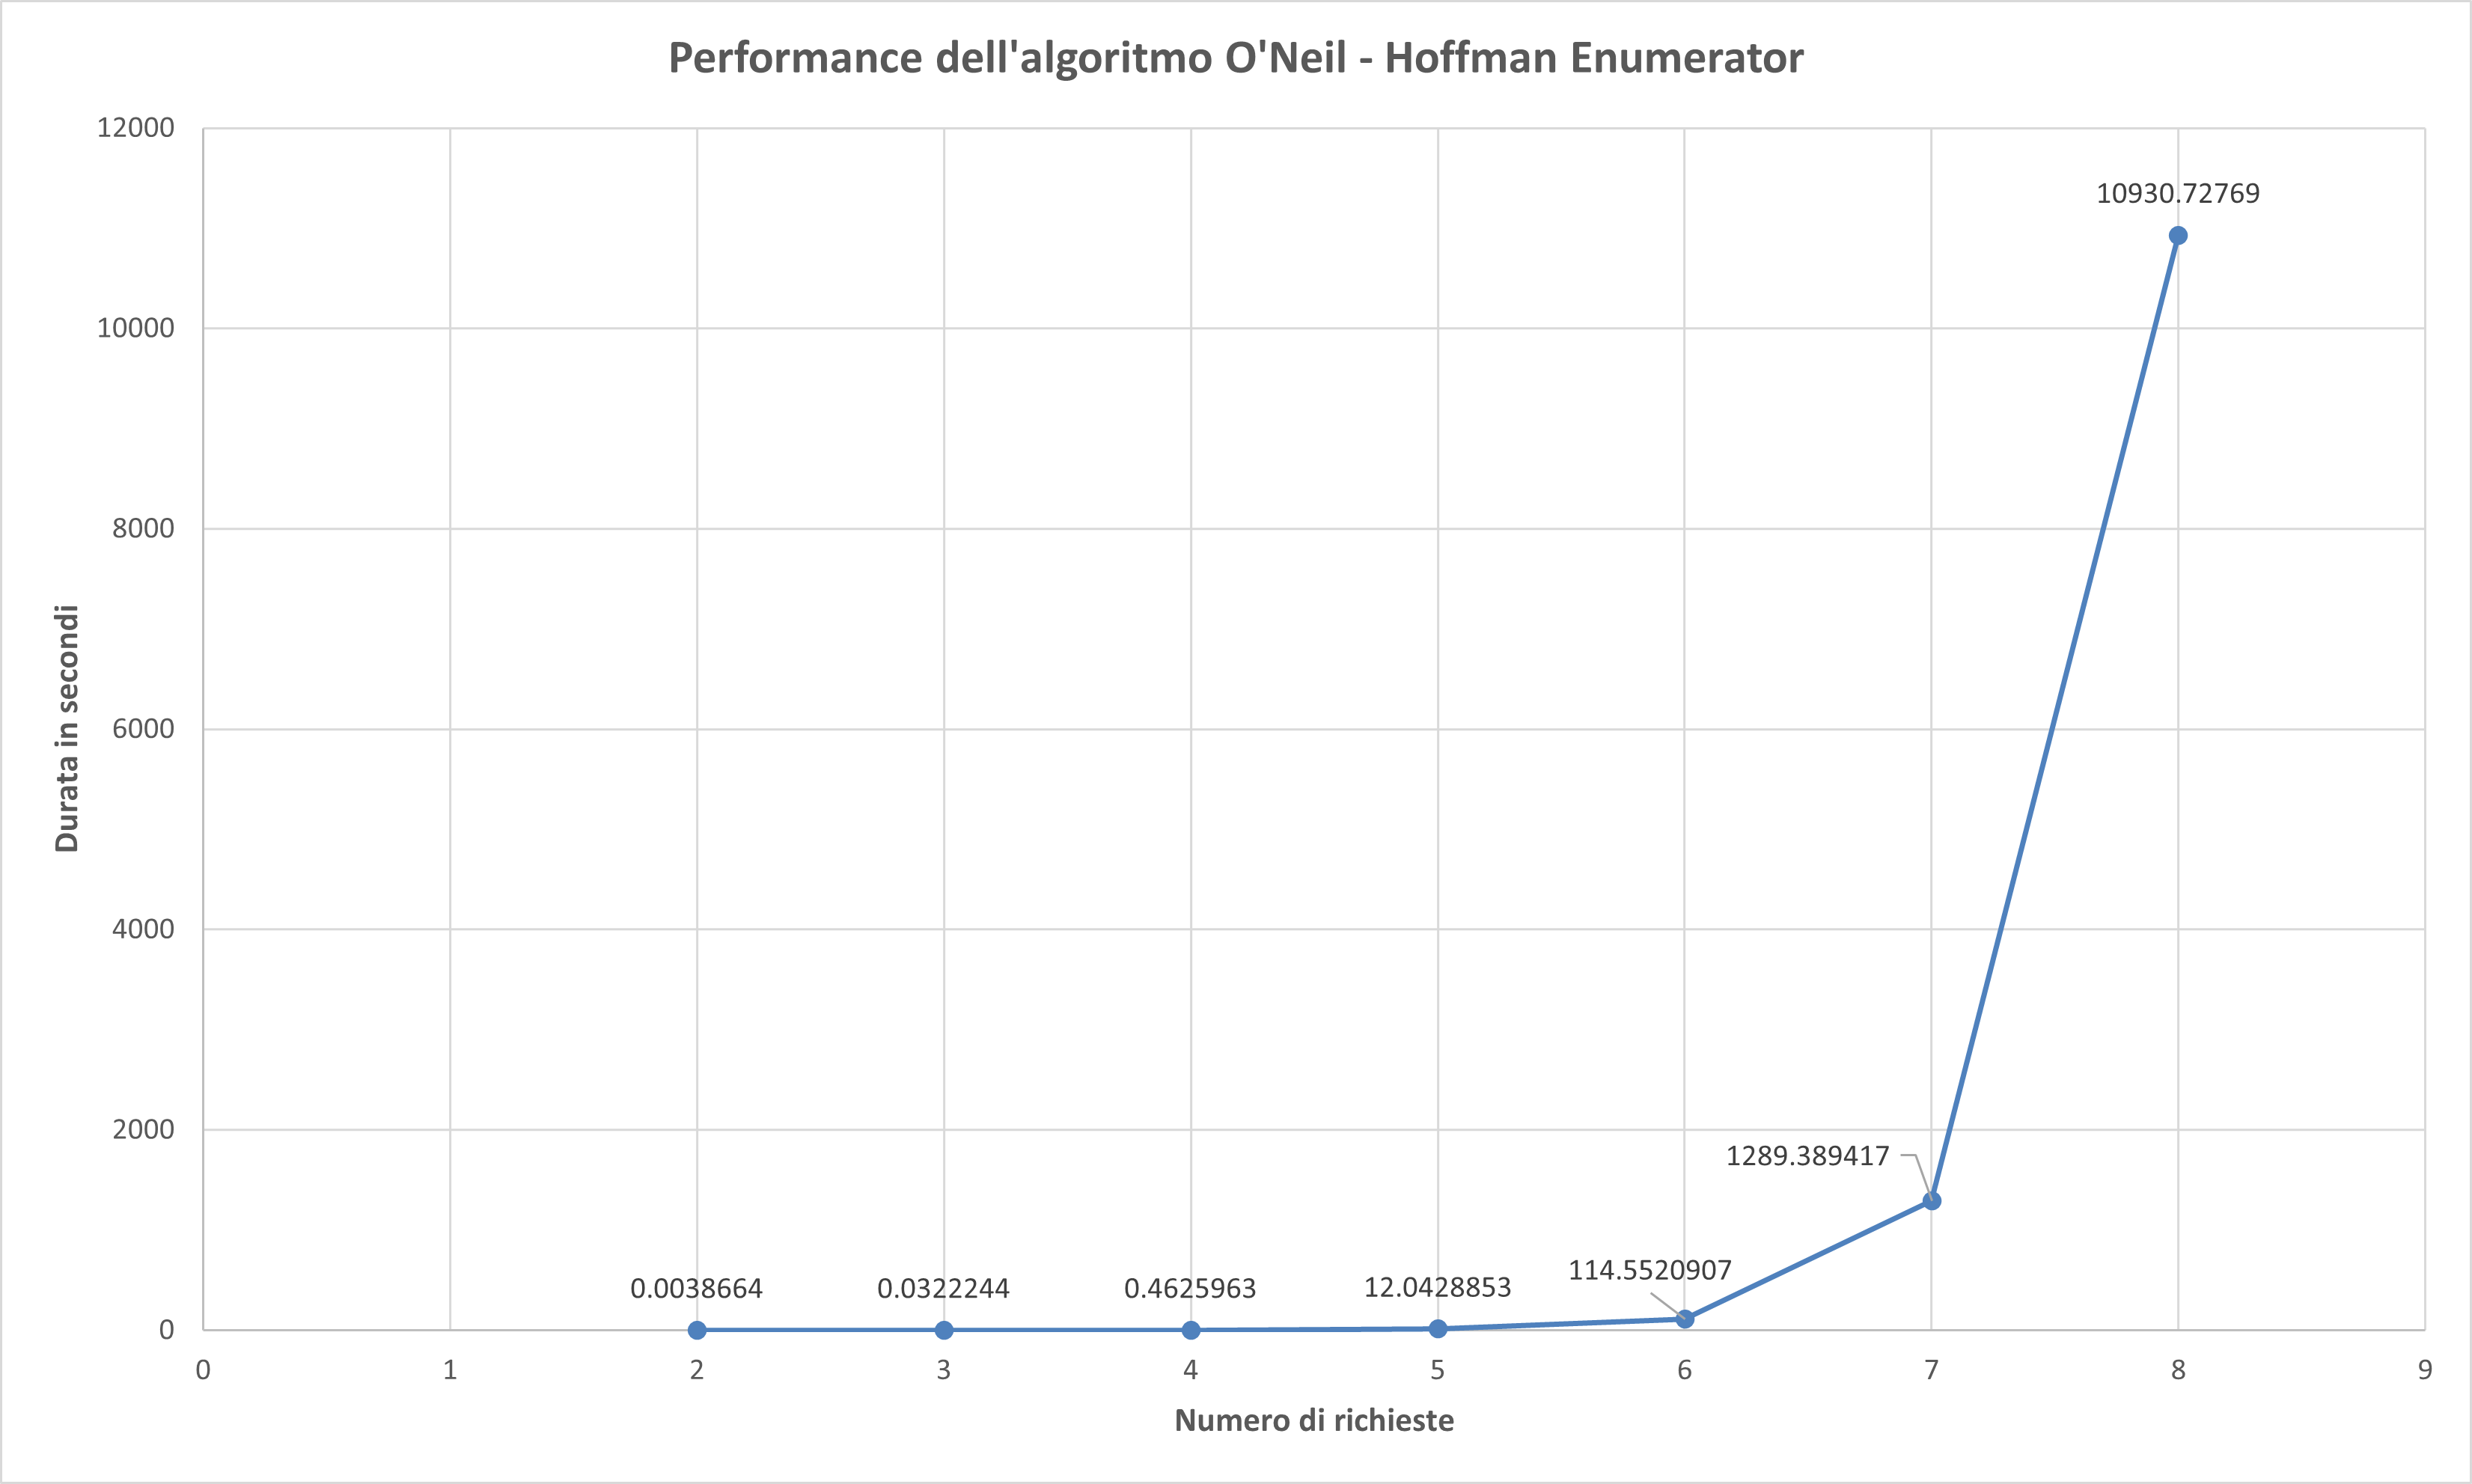
\includegraphics[width=\textwidth]
	{../charts/02 Performance dell'algoritmo O'Neil - Hoffman Enumerator}
	\end{figure}

\end{frame}


\subsection{Confronto}
\begin{frame}[allowframebreaks]{\subsecname}

	\textbf{Performance nel tempo}
      	\begin{figure}[h]
	\centering
	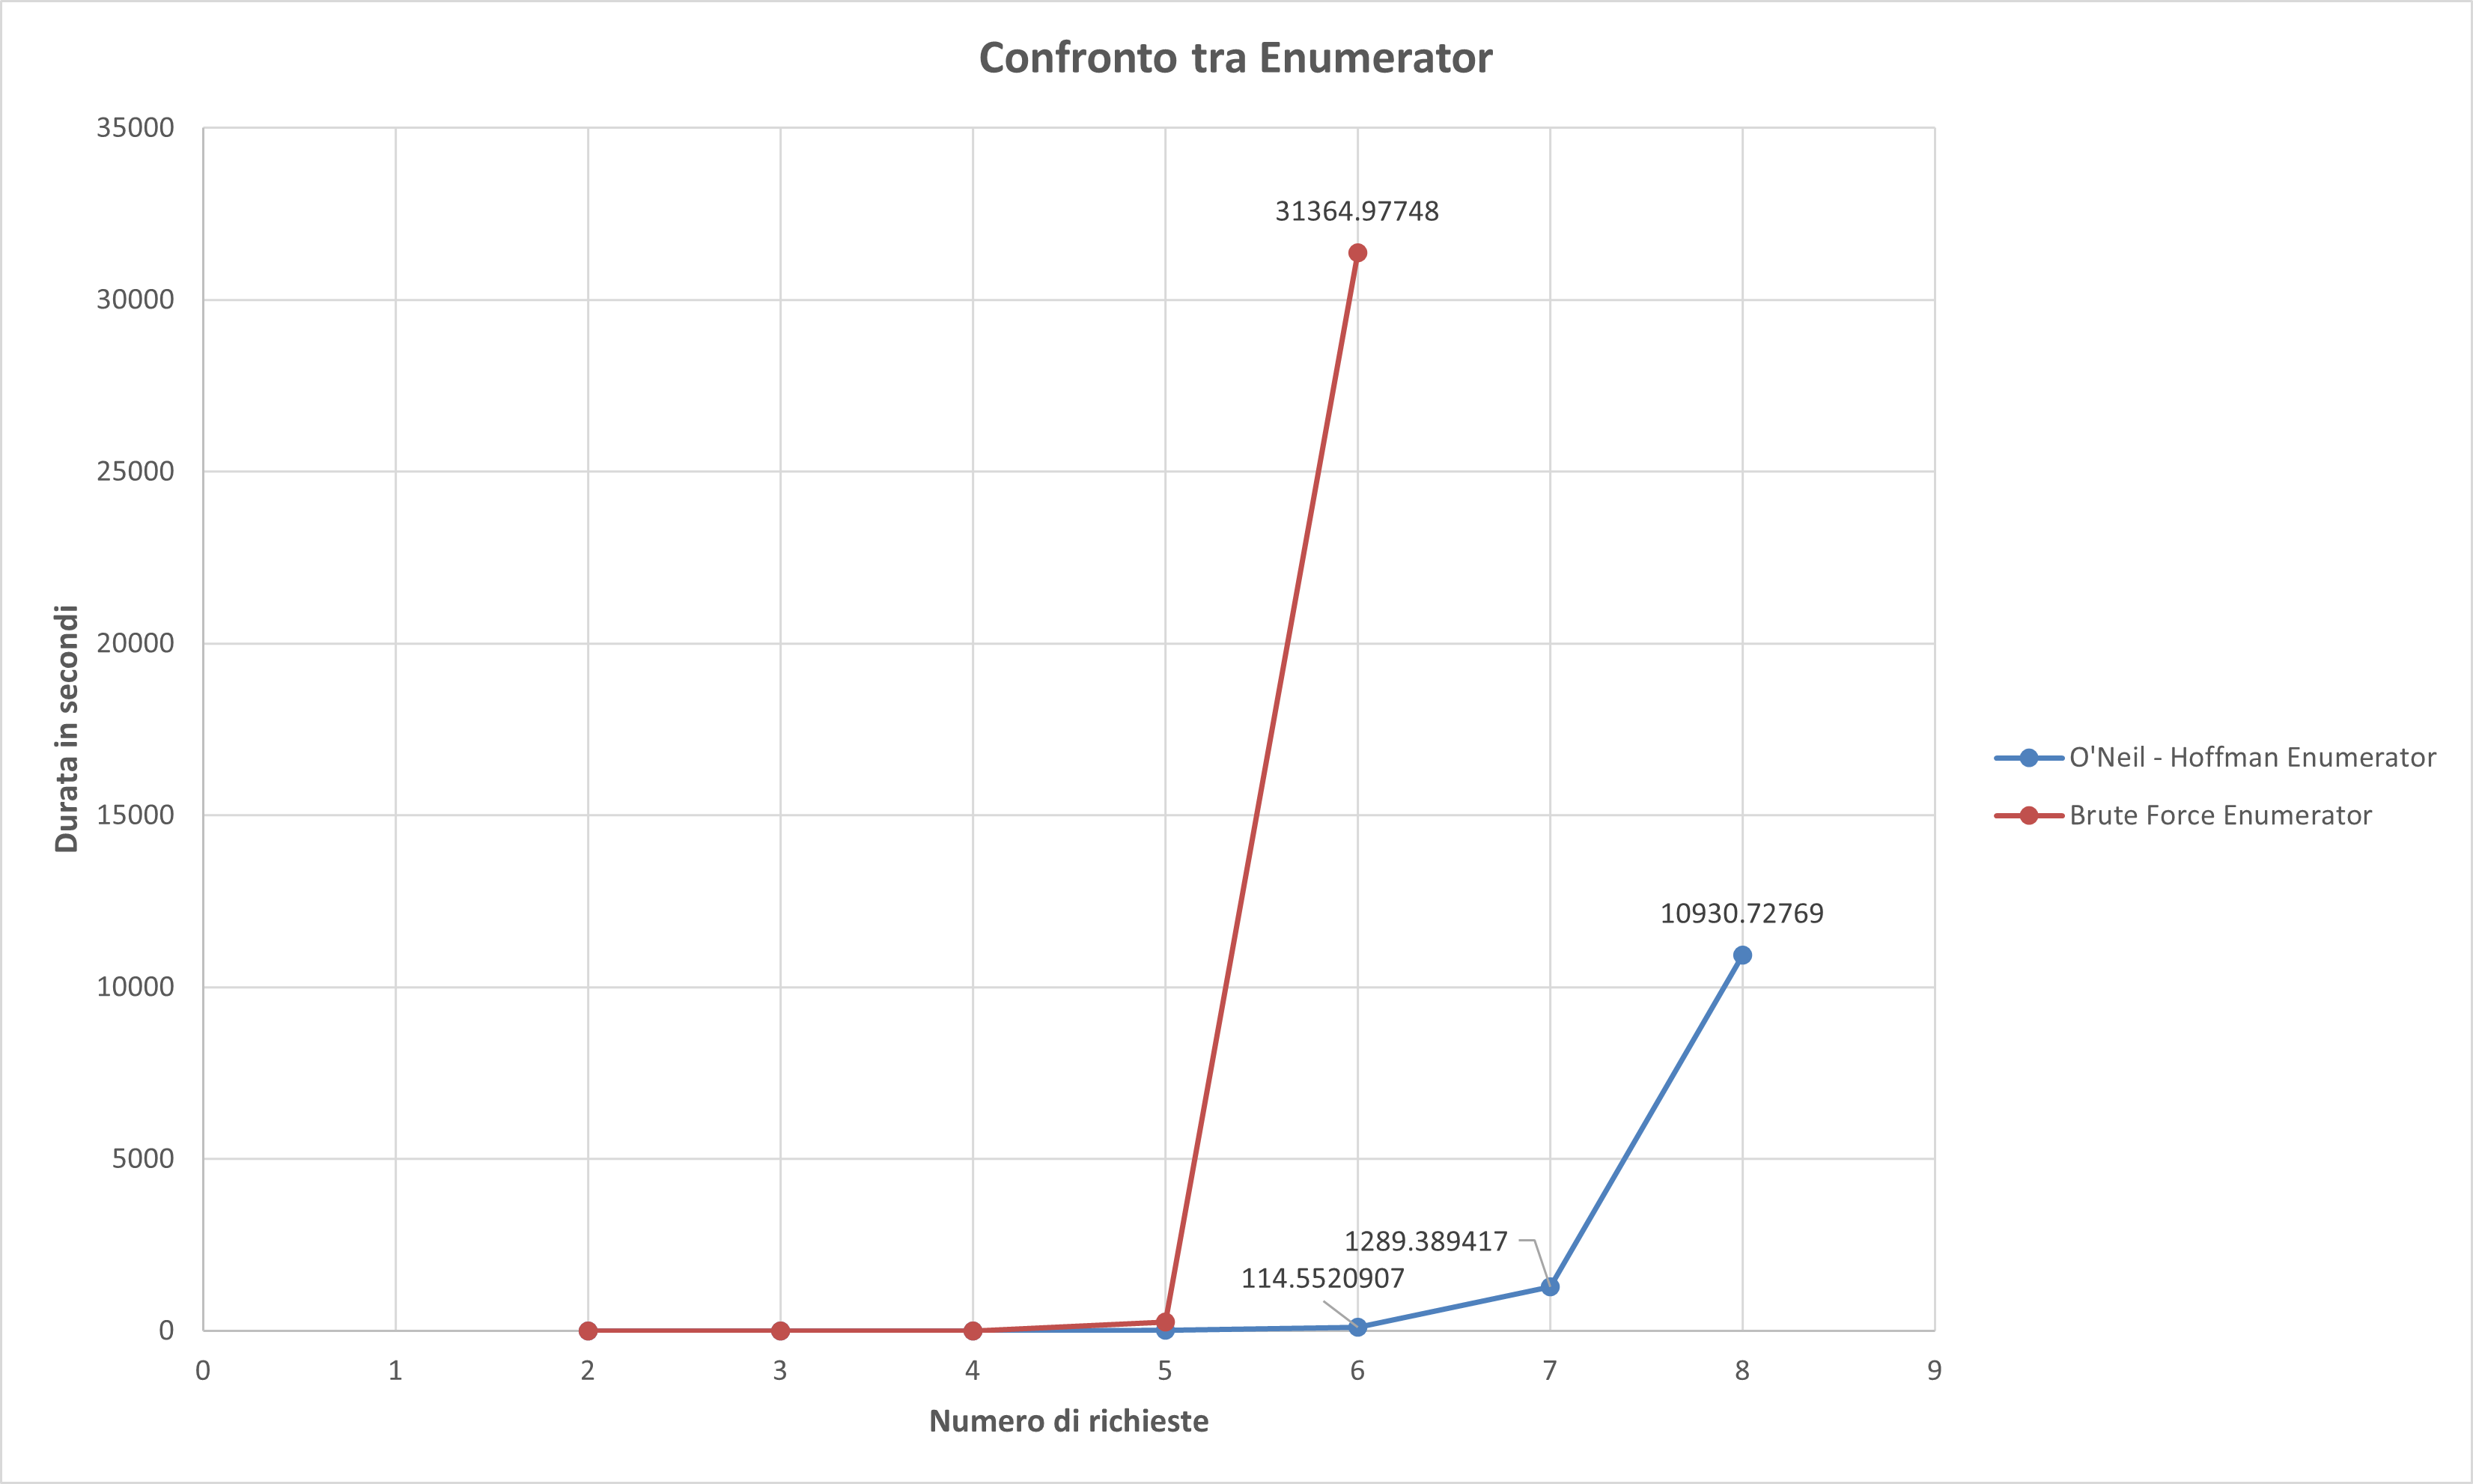
\includegraphics[width=\textwidth]
	{../charts/03 Confronto tra Enumerator}
	\end{figure}

\framebreak

	\textbf{Soluzioni ammissibili esplorate} \\
	I due algoritmi differiscono, oltre che per il tempo di esecuzione anche per il numero di soluzioni ammissibili esplorate
	\begin{table}[h!]
		\centering
		\begin{adjustbox}{max width=\textwidth}
			\begin{tabular}{c c c c c}
				\toprule
				\multirow{2}*{Numero di richieste} & \multicolumn{2}{c}{Brute Force Enumerator} & \multicolumn{2}{c}{O'Neil - Hoffman Enumerator}\\
				& Durata (in secondi) & Soluzioni ammissibili esplorate & Durata (in secondi) & Soluzioni ammissibili esplorate \\
				\midrule
				2 & 0.0153248 & 6 & 0.0038664 & 3 \\
				3 & 0.1156512 & 90 & 0.0322244 & 10 \\
				4 & 2.909126001 & 2520 & 0.4625963 & 3 \\
				5 & 264.0195523 & 113400 & 12.0428853 & 23 \\
				6 & 31364.97748 & 7484400 & 114.5520907 & 115 \\
				7 & N.A. & N.A. & 1289.389417 & 191 \\
				8 & N.A. & N.A. & 10930.72769 & 24 \\
				\bottomrule
			\end{tabular}
		\end{adjustbox}
		\caption{Numero di soluzioni ammissibili esplorate dagli enumeratori}
	\end{table}
	L'enumerazione può essere una tecnica valida per risolvere piccoli TSPPD. Se guidata da alcune informazioni sul problema, l'enumerazione può essere in grado di scoprire rapidamente percorsi validi senza l'onere della formulazione del modello.

\end{frame}

%%%
%%%   ALGORITMI EURISTICI COSTRUTTIVI
%%%

\section{Algoritmi euristici costruttivi}

\subsection{Greedy}
\begin{frame}[allowframebreaks]{\subsecname}

Gli algoritmi greedy (voraci) determinano la soluzione attraverso una sequenza di decisioni parziali (localmente ottime), \emph{senza mai modificare le decisioni gia prese}. \\

Sono di facile implementazione e notevole efficienza computazionale, ma, sia pure con alcune eccezioni di notevole rilievo (Matroidi), \emph{non garantiscono l'ottimalità, e a volte neppure l’ammissibilità della soluzione prodotta.}

\textbf{Definizione di algoritmo greedy} \\
Sia dato il problema di ottimo associato al sistema di insiemi indipendenti $(E,F)$ con funzione obiettivo $c$, si dice Greedy un algoritmo $A$ costruttivo iterativo che costruisce l'insieme $X \in F$, soluzione ammissibile del problema, partendo dall'insieme vuoto ed inserendovi ad ogni passo l’elemento di $E$ più “promettente” fra quelli che non violano l’indipendenza dell'insieme.

\framebreak

\textbf{Procedure Greedy  (template)}

	\begin{itemize}
	
	\item
	Soluzione iniziale $S_0 = \emptyset$
	
	\item
	ad ogni step $k$
	\begin{itemize}
		\item
		seleziona $e_k$ come l’elemento di $E$ più promettente (\emph{criterio best}) tra quelli non ancora esaminati, 
		\item
		valuta se la soluzione parziale $S_k \cup e_k \in F$ (\emph{test di indipendenza} o di ammissibilità delle soluzioni parziali)
	\end{itemize}
	
	\item
	termina avendo esaminato tutto $E$ o quando $S_k$ è massimale ($S_n := S_k$). 
	
	\end{itemize}
	
	Per costruzione $X=S_n$  è massimale. 	La complessità di “Greedy” dipende dalla complessità delle procedure \emph{Best} e \emph{Ind}, essendo predefinito il numero massimo di iterazioni ($n$). Per costruire un algoritmo greedy è sufficiente definire $E$ ed $F$, e specificare \emph{Best} e \emph{Ind} nell’ambito del template.

	\textbf{Codice} \\
	\href{https://github.com/michele-vaccari/TSP-con-pick-up-and-delivery/blob/main/src/tsppd/solver/greedyTemplate.py}{https://github.com/michele-vaccari/TSP-con-pick-up-and-delivery/blob/main/src/tsppd/solver/greedyTemplate.py}
\end{frame}

\subsection{Greedy Pickup First}
\begin{frame}[allowframebreaks]{\subsecname}
	\textbf{Definizione del criterio best e test di ammissibilità}
      \begin{description}[style=unboxed,leftmargin=0cm]
        \item[criterio best] seleziono prima i nodi pick-up in ordine di richiesta, poi i nodi di delivery in ordine di richiesta
	  \item[test di ammissibilità] verifico che le precedenze tra i nodi siano sempre rispettate (lo sono per costruzione)
      \end{description}

	\textbf{Codice} \\
		\href{https://github.com/michele-vaccari/TSP-con-pick-up-and-delivery/blob/main/src/tsppd/solver/greedyPickupFirst.py}{https://github.com/michele-vaccari/TSP-con-pick-up-and-delivery/blob/main/src/tsppd/solver/greedyPickupFirst.py}

\framebreak

\textbf{Esempio}
\begin{columns}[T,onlytextwidth]
	\column{0.5\textwidth}
	\begin{figure}[h]
	\centering
	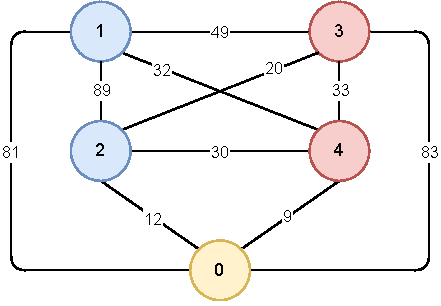
\includegraphics[height=0.4\textheight]
	{../images/graph-tsppd-with-two-customers}	
	\caption{Istanza iniziale}
	\end{figure}
	\column{0.5\textwidth}
	\begin{figure}[h]
	\centering
	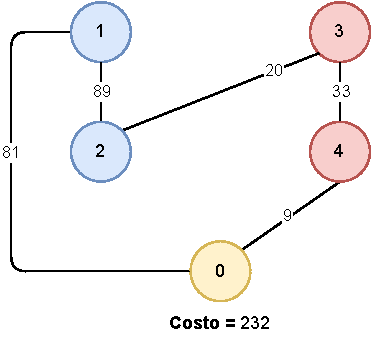
\includegraphics[height=0.4\textheight]
	{../images/graph-greedy-pickup-first-solution-tsppd-with-two-customers}	
	\caption{Soluzione generata}
	\end{figure}
\end{columns}

\framebreak

	\textbf{Performance nel tempo}
      	\begin{figure}[h]
	\centering
	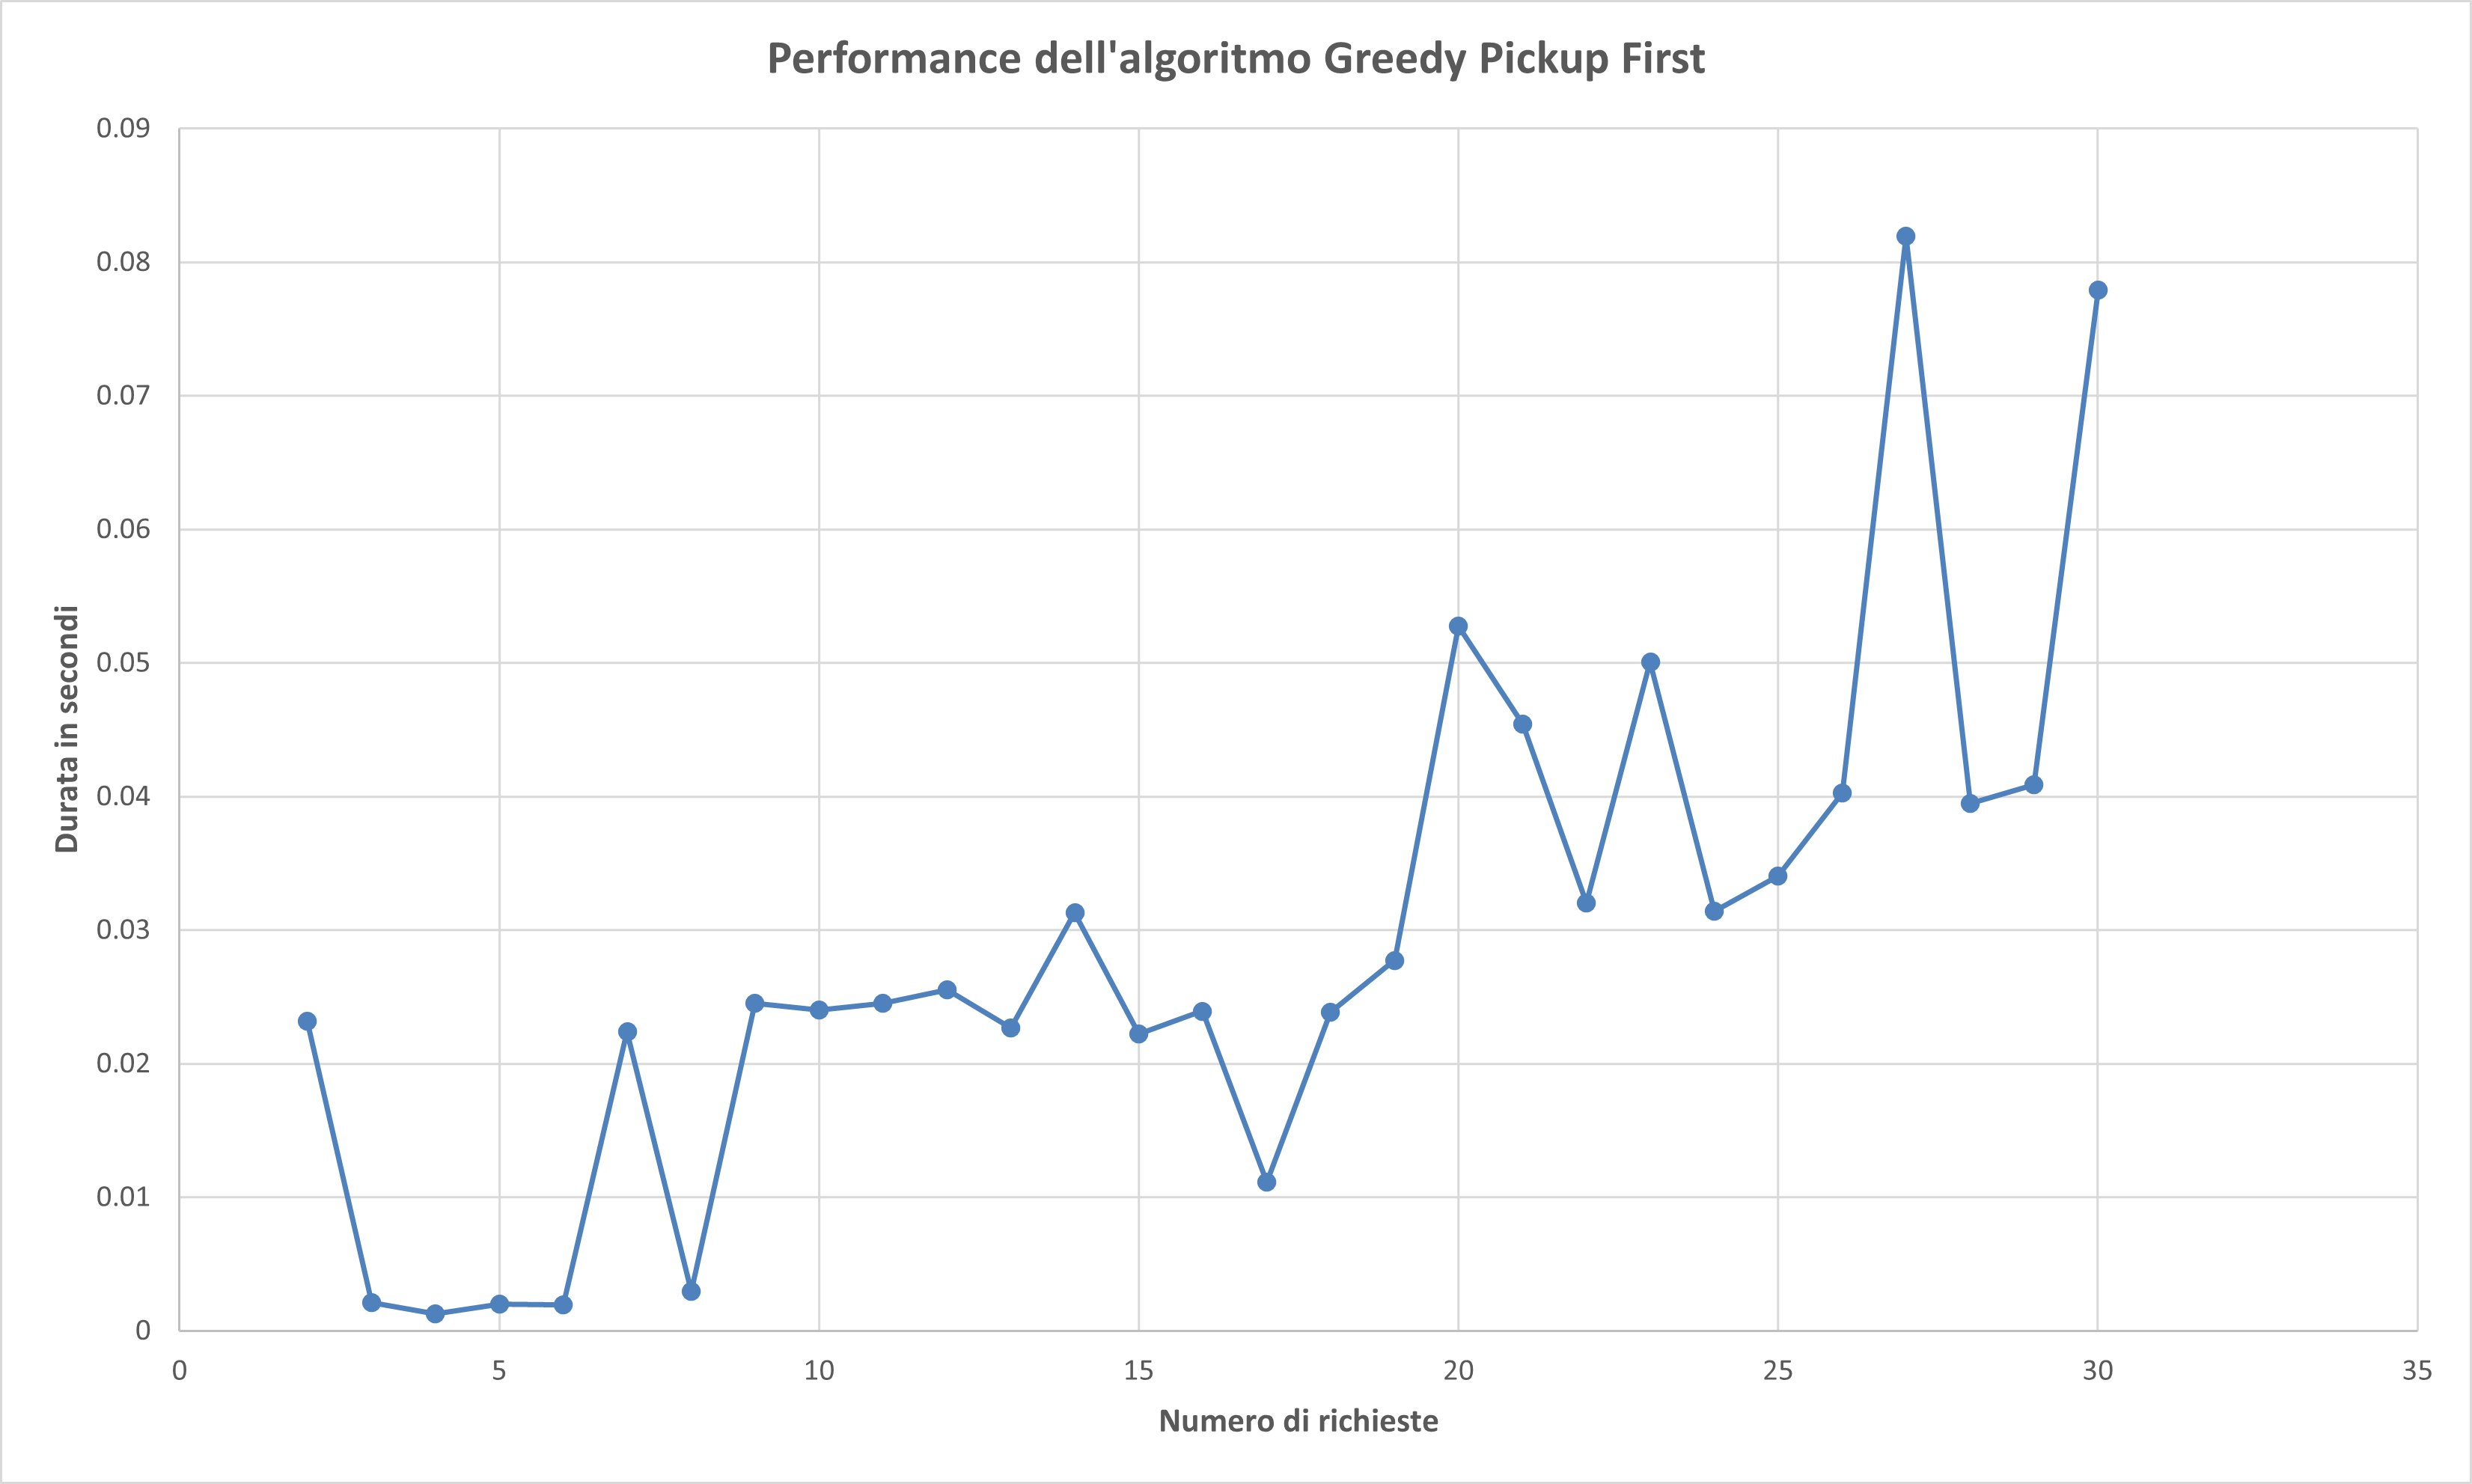
\includegraphics[width=\textwidth]
	{../charts/04 Performance dell'algoritmo Greedy Pickup First}
	\end{figure}

\end{frame}

\subsection{Greedy Request Order}
\begin{frame}[allowframebreaks]{\subsecname}
	\textbf{Definizione del criterio best e test di ammissibilità}
      \begin{description}[style=unboxed,leftmargin=0cm]
        \item[criterio best] seleziono prima i nodi pick-up e di delivery in ordine di richiesta
	  \item[test di ammissibilità] verifico che le precedenze tra i nodi siano sempre rispettate (lo sono per costruzione)
      \end{description}

	\textbf{Codice} \\
		\href{https://github.com/michele-vaccari/TSP-con-pick-up-and-delivery/blob/main/src/tsppd/solver/greedyRequestOrder.py}{https://github.com/michele-vaccari/TSP-con-pick-up-and-delivery/blob/main/src/tsppd/solver/greedyRequestOrder.py}

\framebreak

\textbf{Esempio}
\begin{columns}[T,onlytextwidth]
	\column{0.5\textwidth}
	\begin{figure}[h]
	\centering
	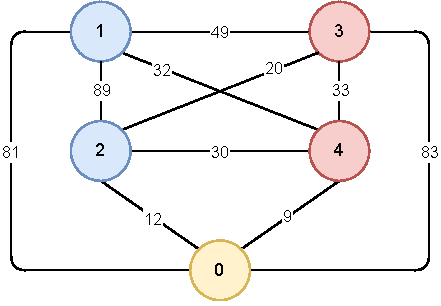
\includegraphics[height=0.4\textheight]
	{../images/graph-tsppd-with-two-customers}	
	\caption{Istanza iniziale}
	\end{figure}
	\column{0.5\textwidth}
	\begin{figure}[h]
	\centering
	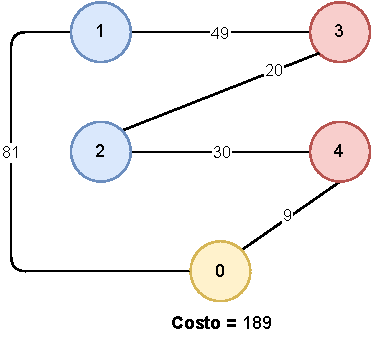
\includegraphics[height=0.4\textheight]
	{../images/graph-greedy-request-order-solution-tsppd-with-two-customers}	
	\caption{Soluzione generata}
	\end{figure}
\end{columns}

\textbf{N.B.} In questo caso la soluzione generata è la soluzione ottima

\framebreak

	\textbf{Performance nel tempo}
      	\begin{figure}[h]
	\centering
	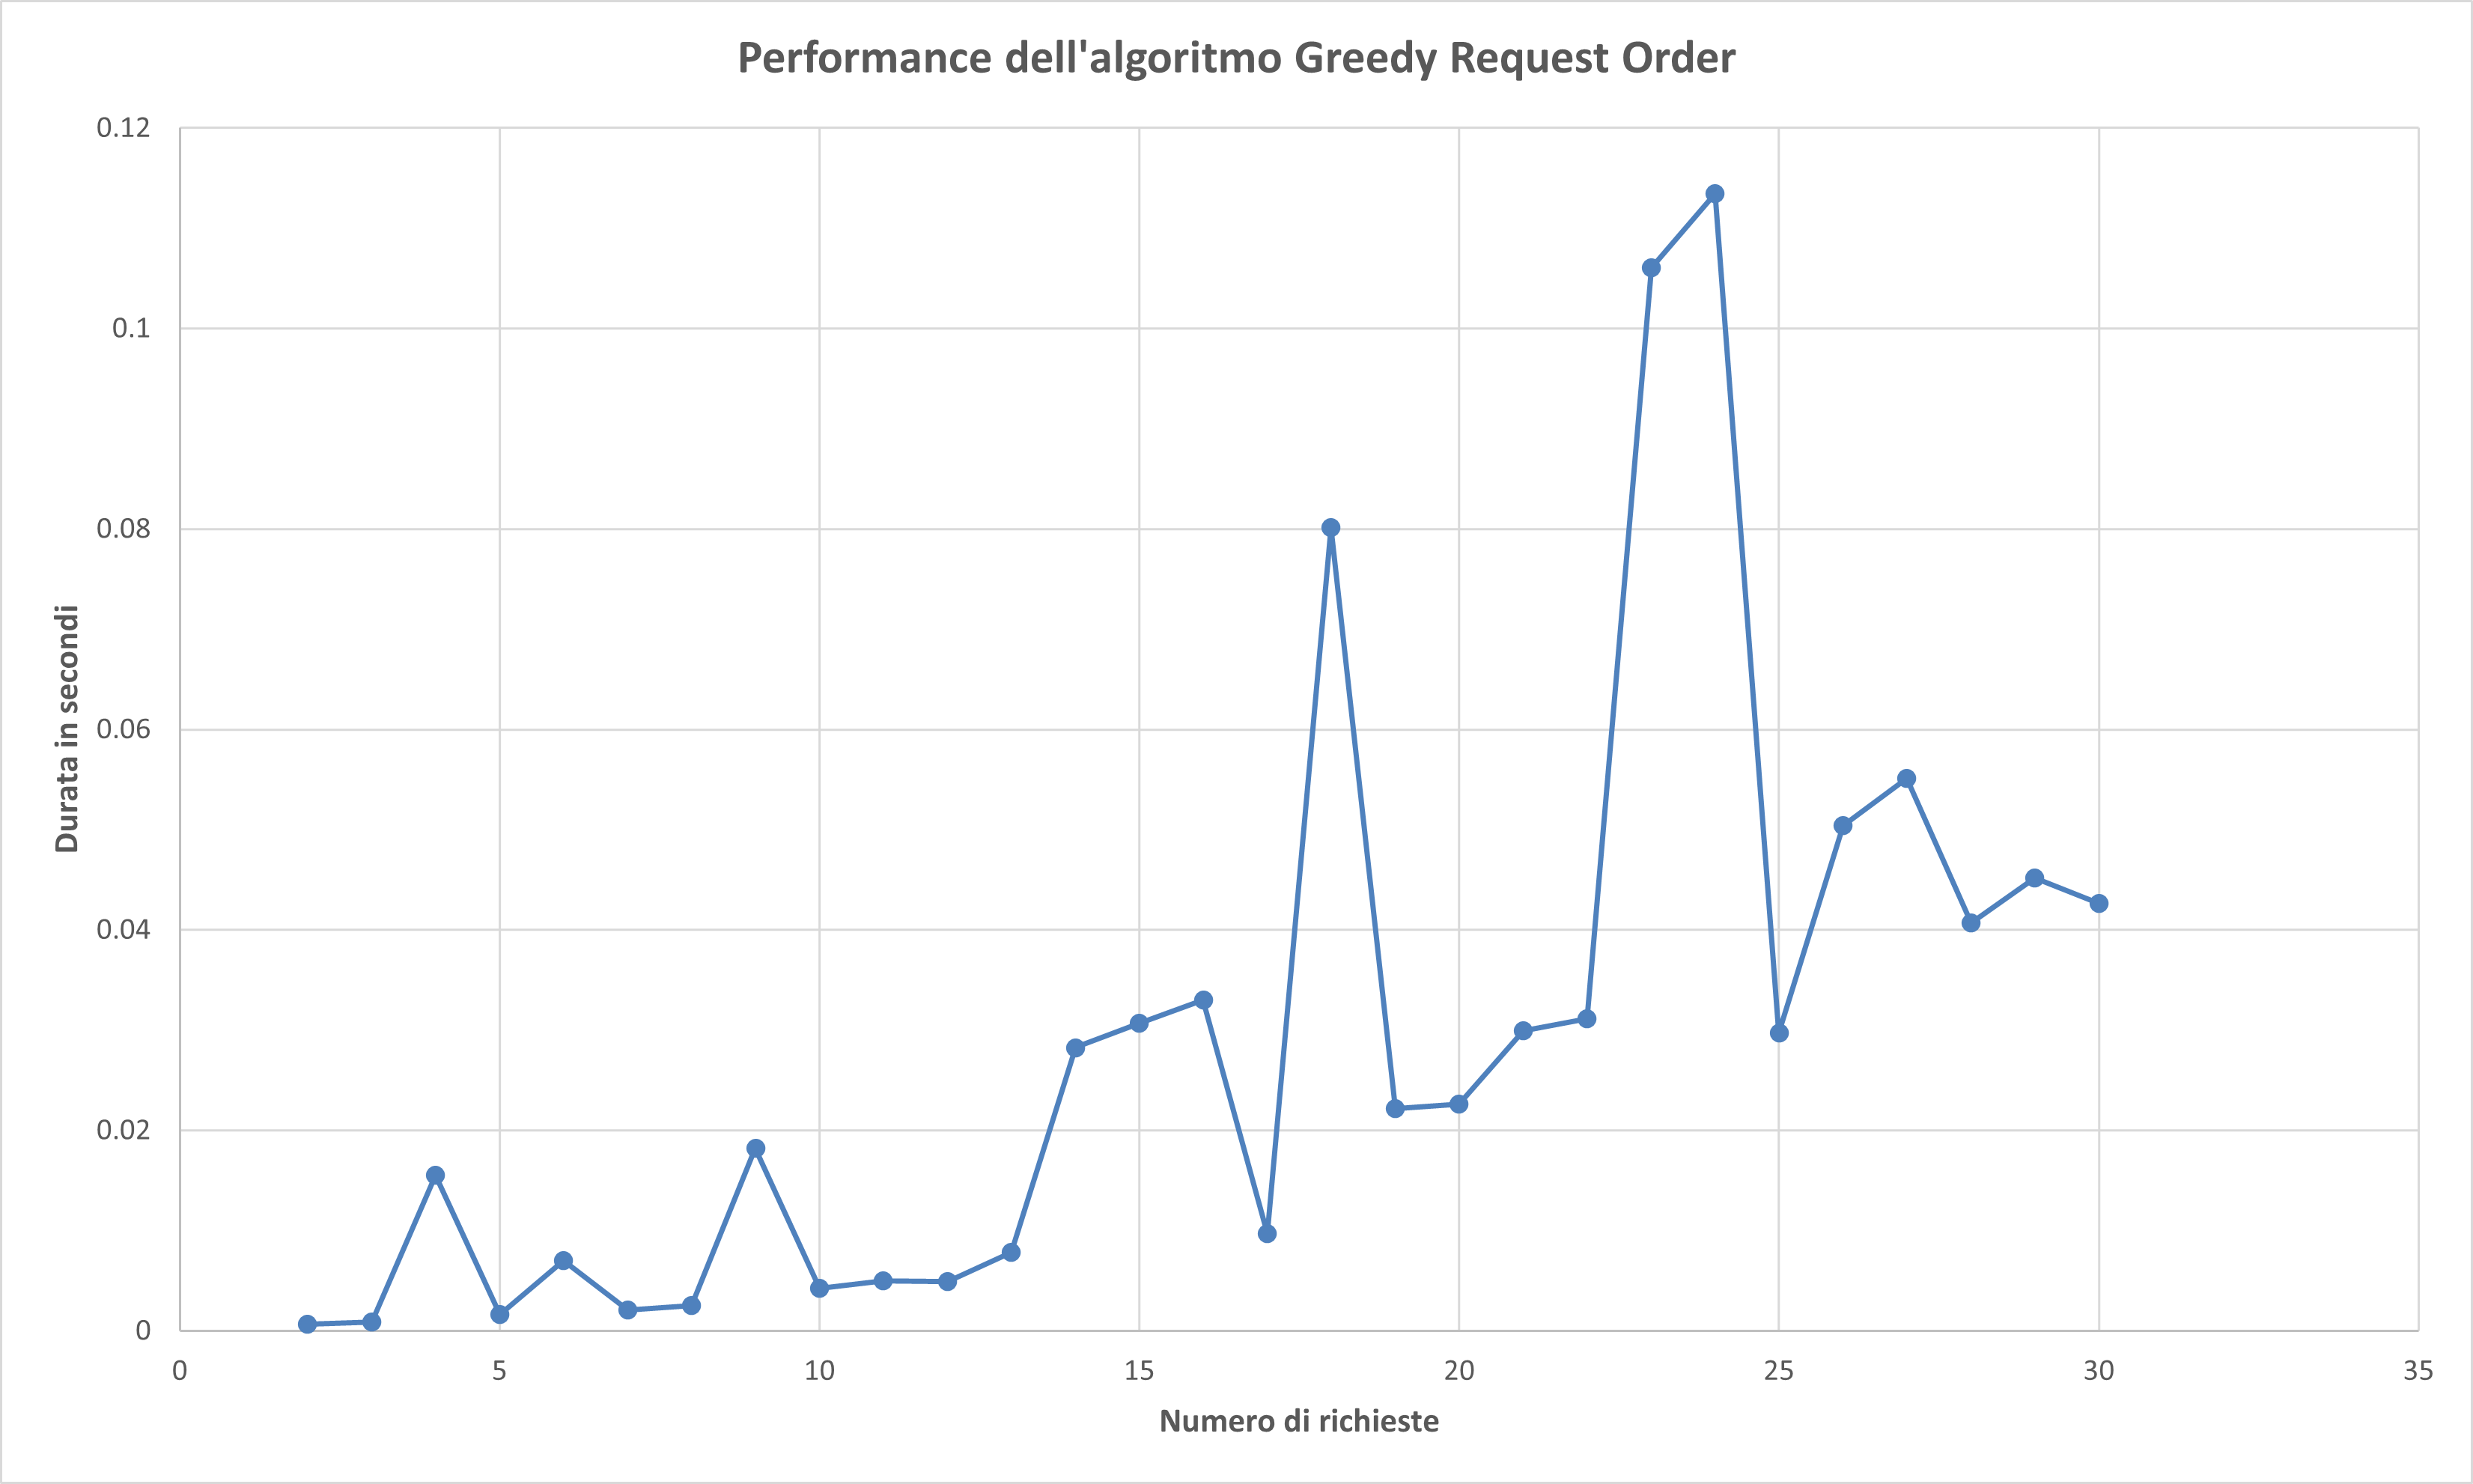
\includegraphics[width=\textwidth]
	{../charts/05 Performance dell'algoritmo Greedy Request Order}
	\end{figure}

\end{frame}

\subsection{Greedy Nearest Neighbor}
\begin{frame}[allowframebreaks]{\subsecname}
	\textbf{Definizione del criterio best e test di ammissibilità}
      \begin{description}[style=unboxed,leftmargin=0cm]
        \item[criterio best] seleziono il nodo successivo più vicino rispetto al nodo corrente
	  \item[test di ammissibilità] verifico che le precedenze tra i nodi siano sempre rispettate
      \end{description}

	\textbf{Codice} \\
		\href{https://github.com/michele-vaccari/TSP-con-pick-up-and-delivery/blob/main/src/tsppd/solver/greedyNearestNeighbor.py}{https://github.com/michele-vaccari/TSP-con-pick-up-and-delivery/blob/main/src/tsppd/solver/greedyNearestNeighbor.py}

\framebreak

\textbf{Esempio}
\begin{columns}[T,onlytextwidth]
	\column{0.5\textwidth}
	\begin{figure}[h]
	\centering
	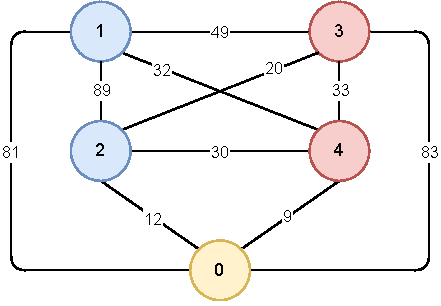
\includegraphics[height=0.4\textheight]
	{../images/graph-tsppd-with-two-customers}	
	\caption{Istanza iniziale}
	\end{figure}
	\column{0.5\textwidth}
	\begin{figure}[h]
	\centering
	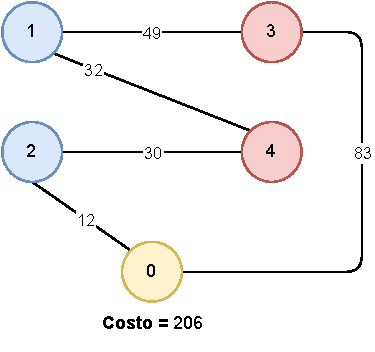
\includegraphics[height=0.4\textheight]
	{../images/graph-greedy-nearest-neighbor-solution-tsppd-with-two-customers}	
	\caption{Soluzione generata}
	\end{figure}
\end{columns}

\framebreak

	\textbf{Performance nel tempo}
      	\begin{figure}[h]
	\centering
	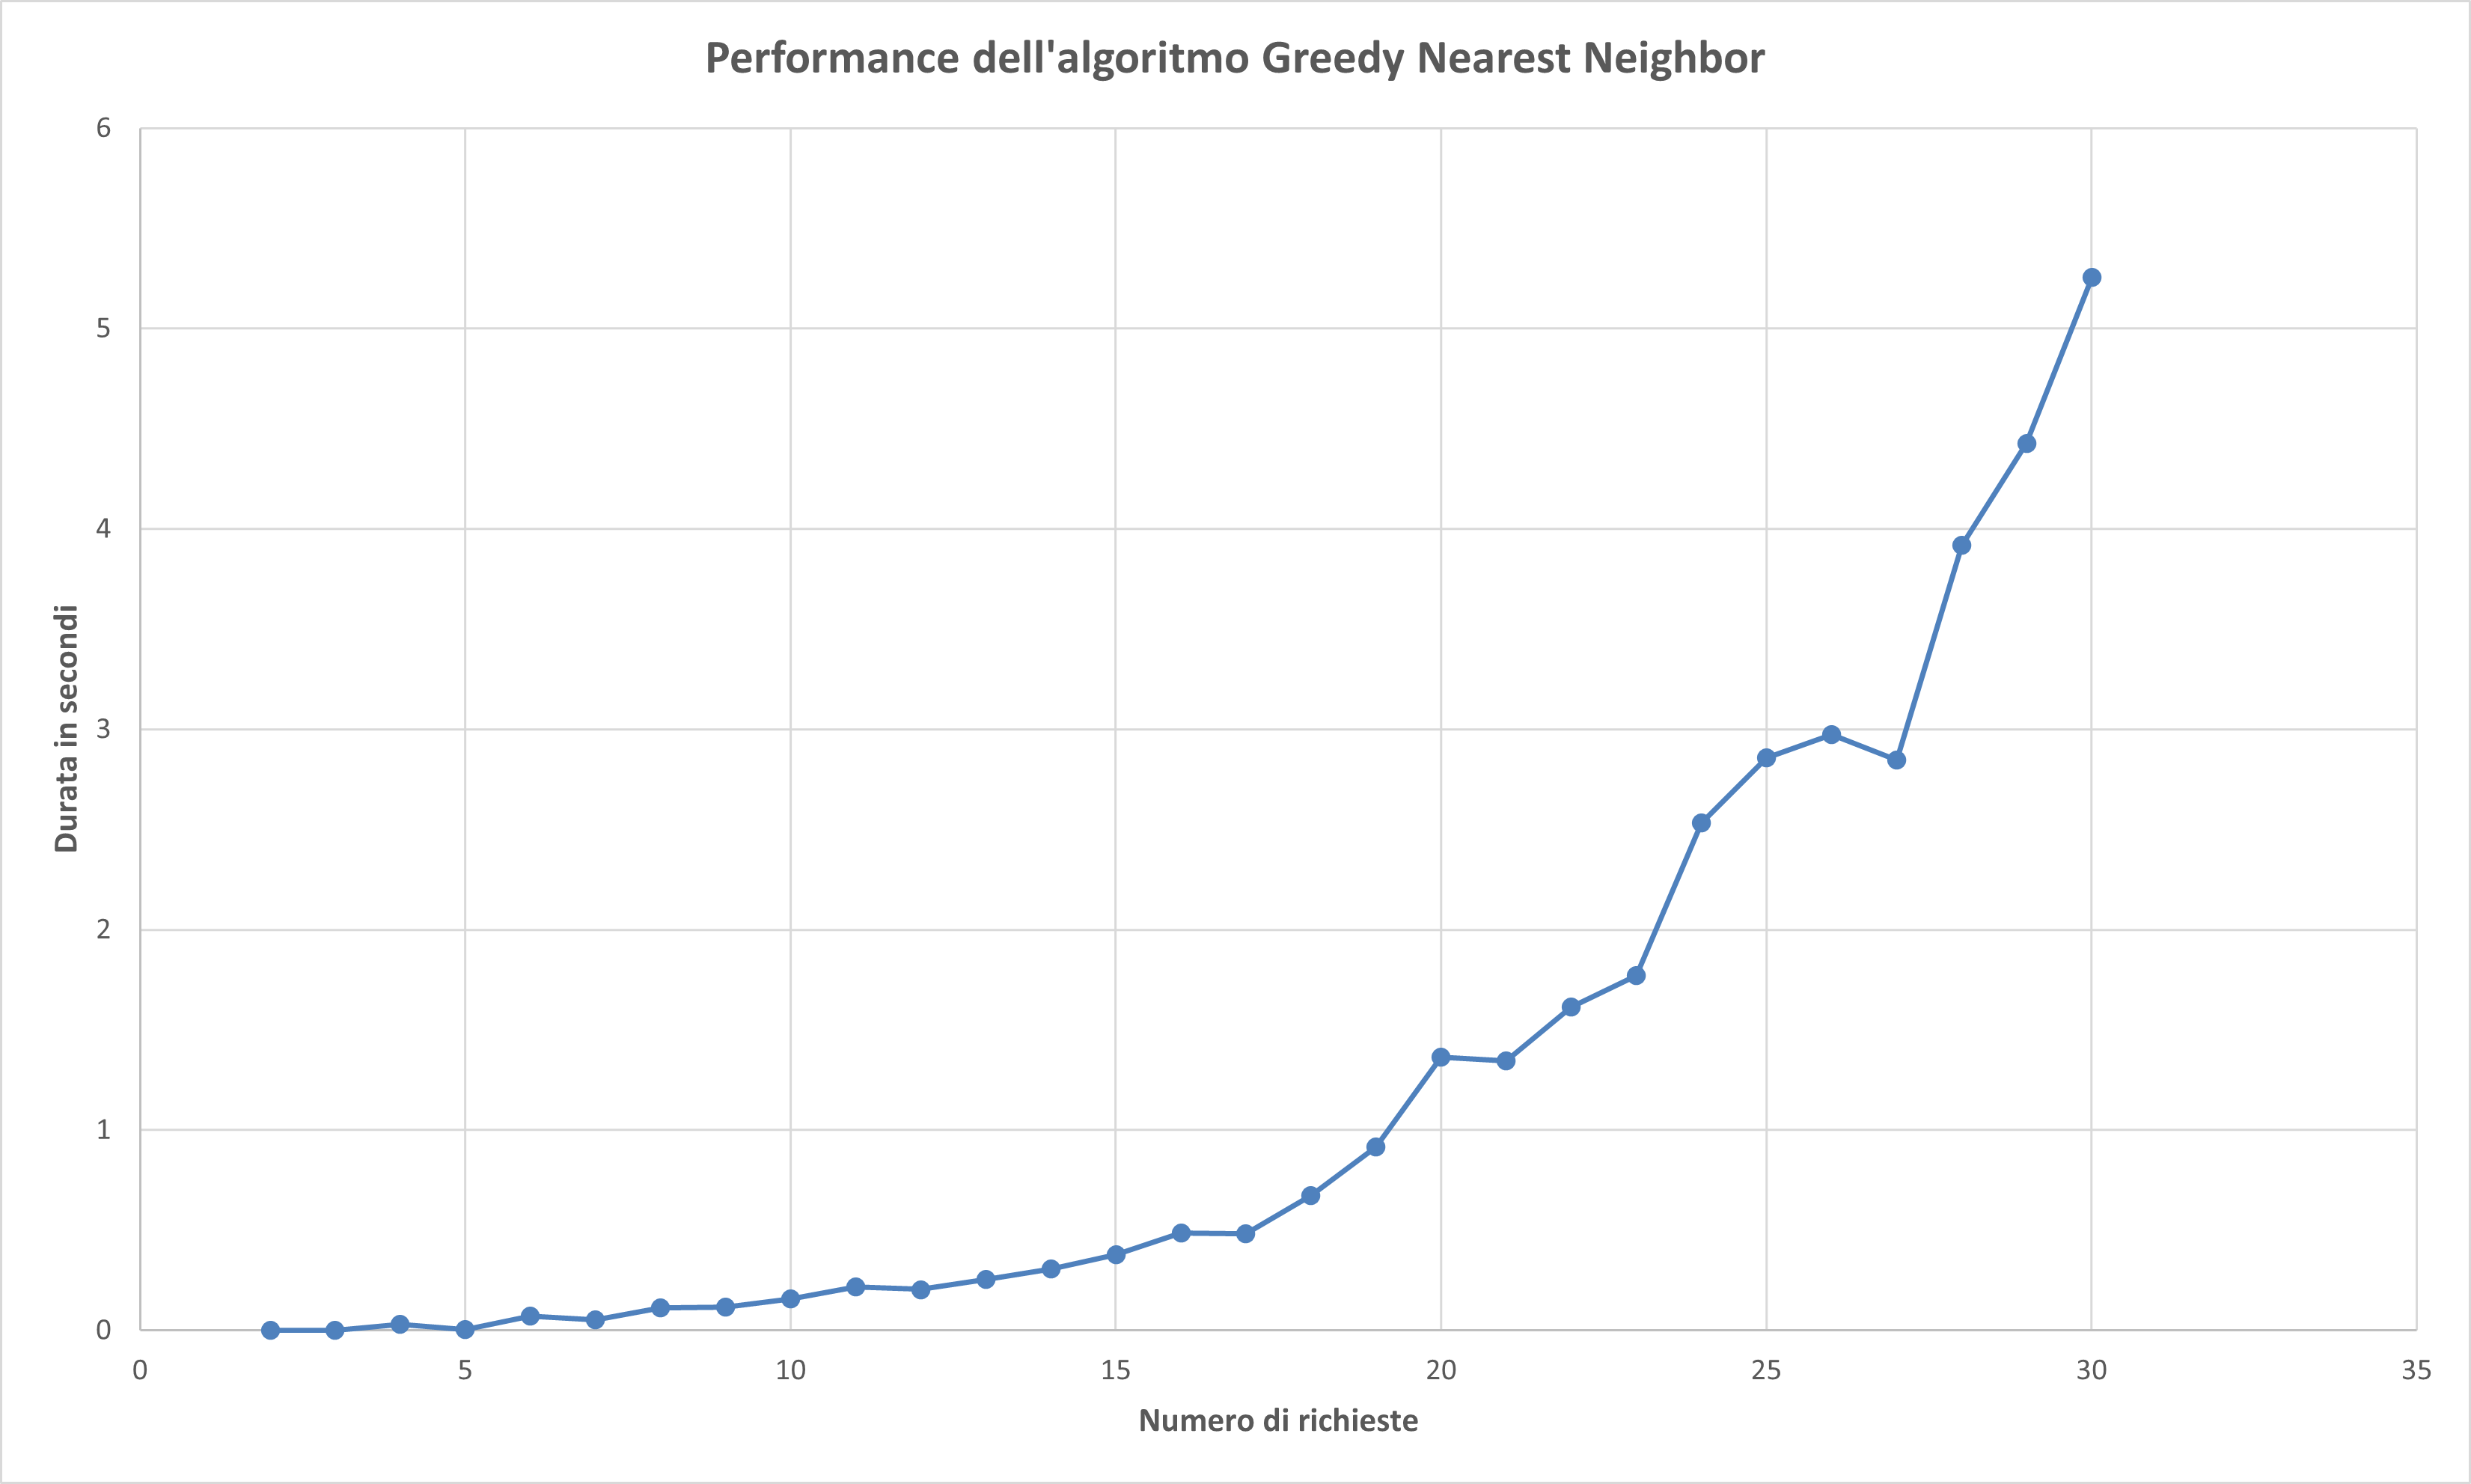
\includegraphics[width=\textwidth]
	{../charts/06 Performance dell'algoritmo Greedy Nearest Neighbor}
	\end{figure}

\end{frame}

\subsection{Greedy Random}
\begin{frame}[allowframebreaks]{\subsecname}
	\textbf{Definizione del criterio best e test di ammissibilità}
	\begin{description}[style=unboxed,leftmargin=0cm]
		\item[criterio best] seleziono il nodo successivo a caso
		\item[test di ammissibilità] verifico che le precedenze tra i nodi siano sempre rispettate
	\end{description}

	\textbf{Codice} \\
		\href{https://github.com/michele-vaccari/TSP-con-pick-up-and-delivery/blob/main/src/tsppd/solver/greedyRandom.py}{https://github.com/michele-vaccari/TSP-con-pick-up-and-delivery/blob/main/src/tsppd/solver/greedyRandom.py}

\framebreak

	\textbf{Esempio}
	\begin{figure}[h]
	\centering
	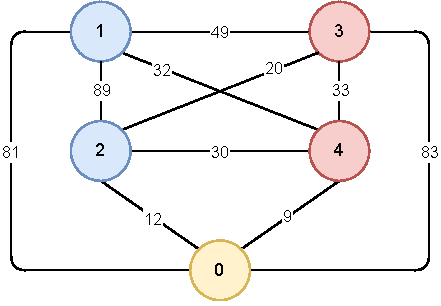
\includegraphics[width=0.4\textwidth]
	{../images/graph-tsppd-with-two-customers}	
	\caption{Istanza iniziale}
	\end{figure}

\framebreak

	\textbf{Esecuzione}
      	\begin{figure}[h]
	\centering
	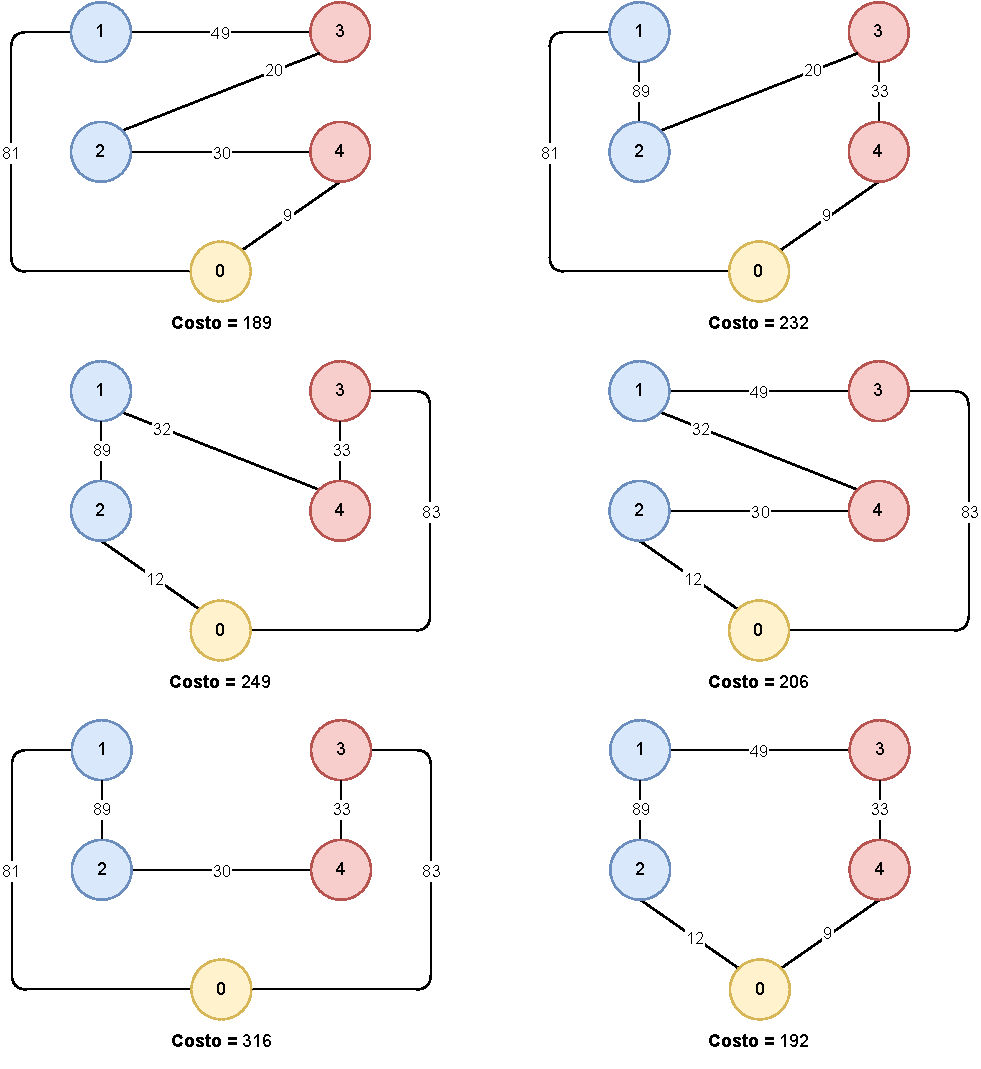
\includegraphics[width=0.45\textwidth]
	{../images/graph-all-solutions-with-cost-tsppd-with-two-customers}	
	\caption{Possibili soluzioni generate}
	\end{figure}

\framebreak

	\textbf{Performance nel tempo}
      	\begin{figure}[h]
	\centering
	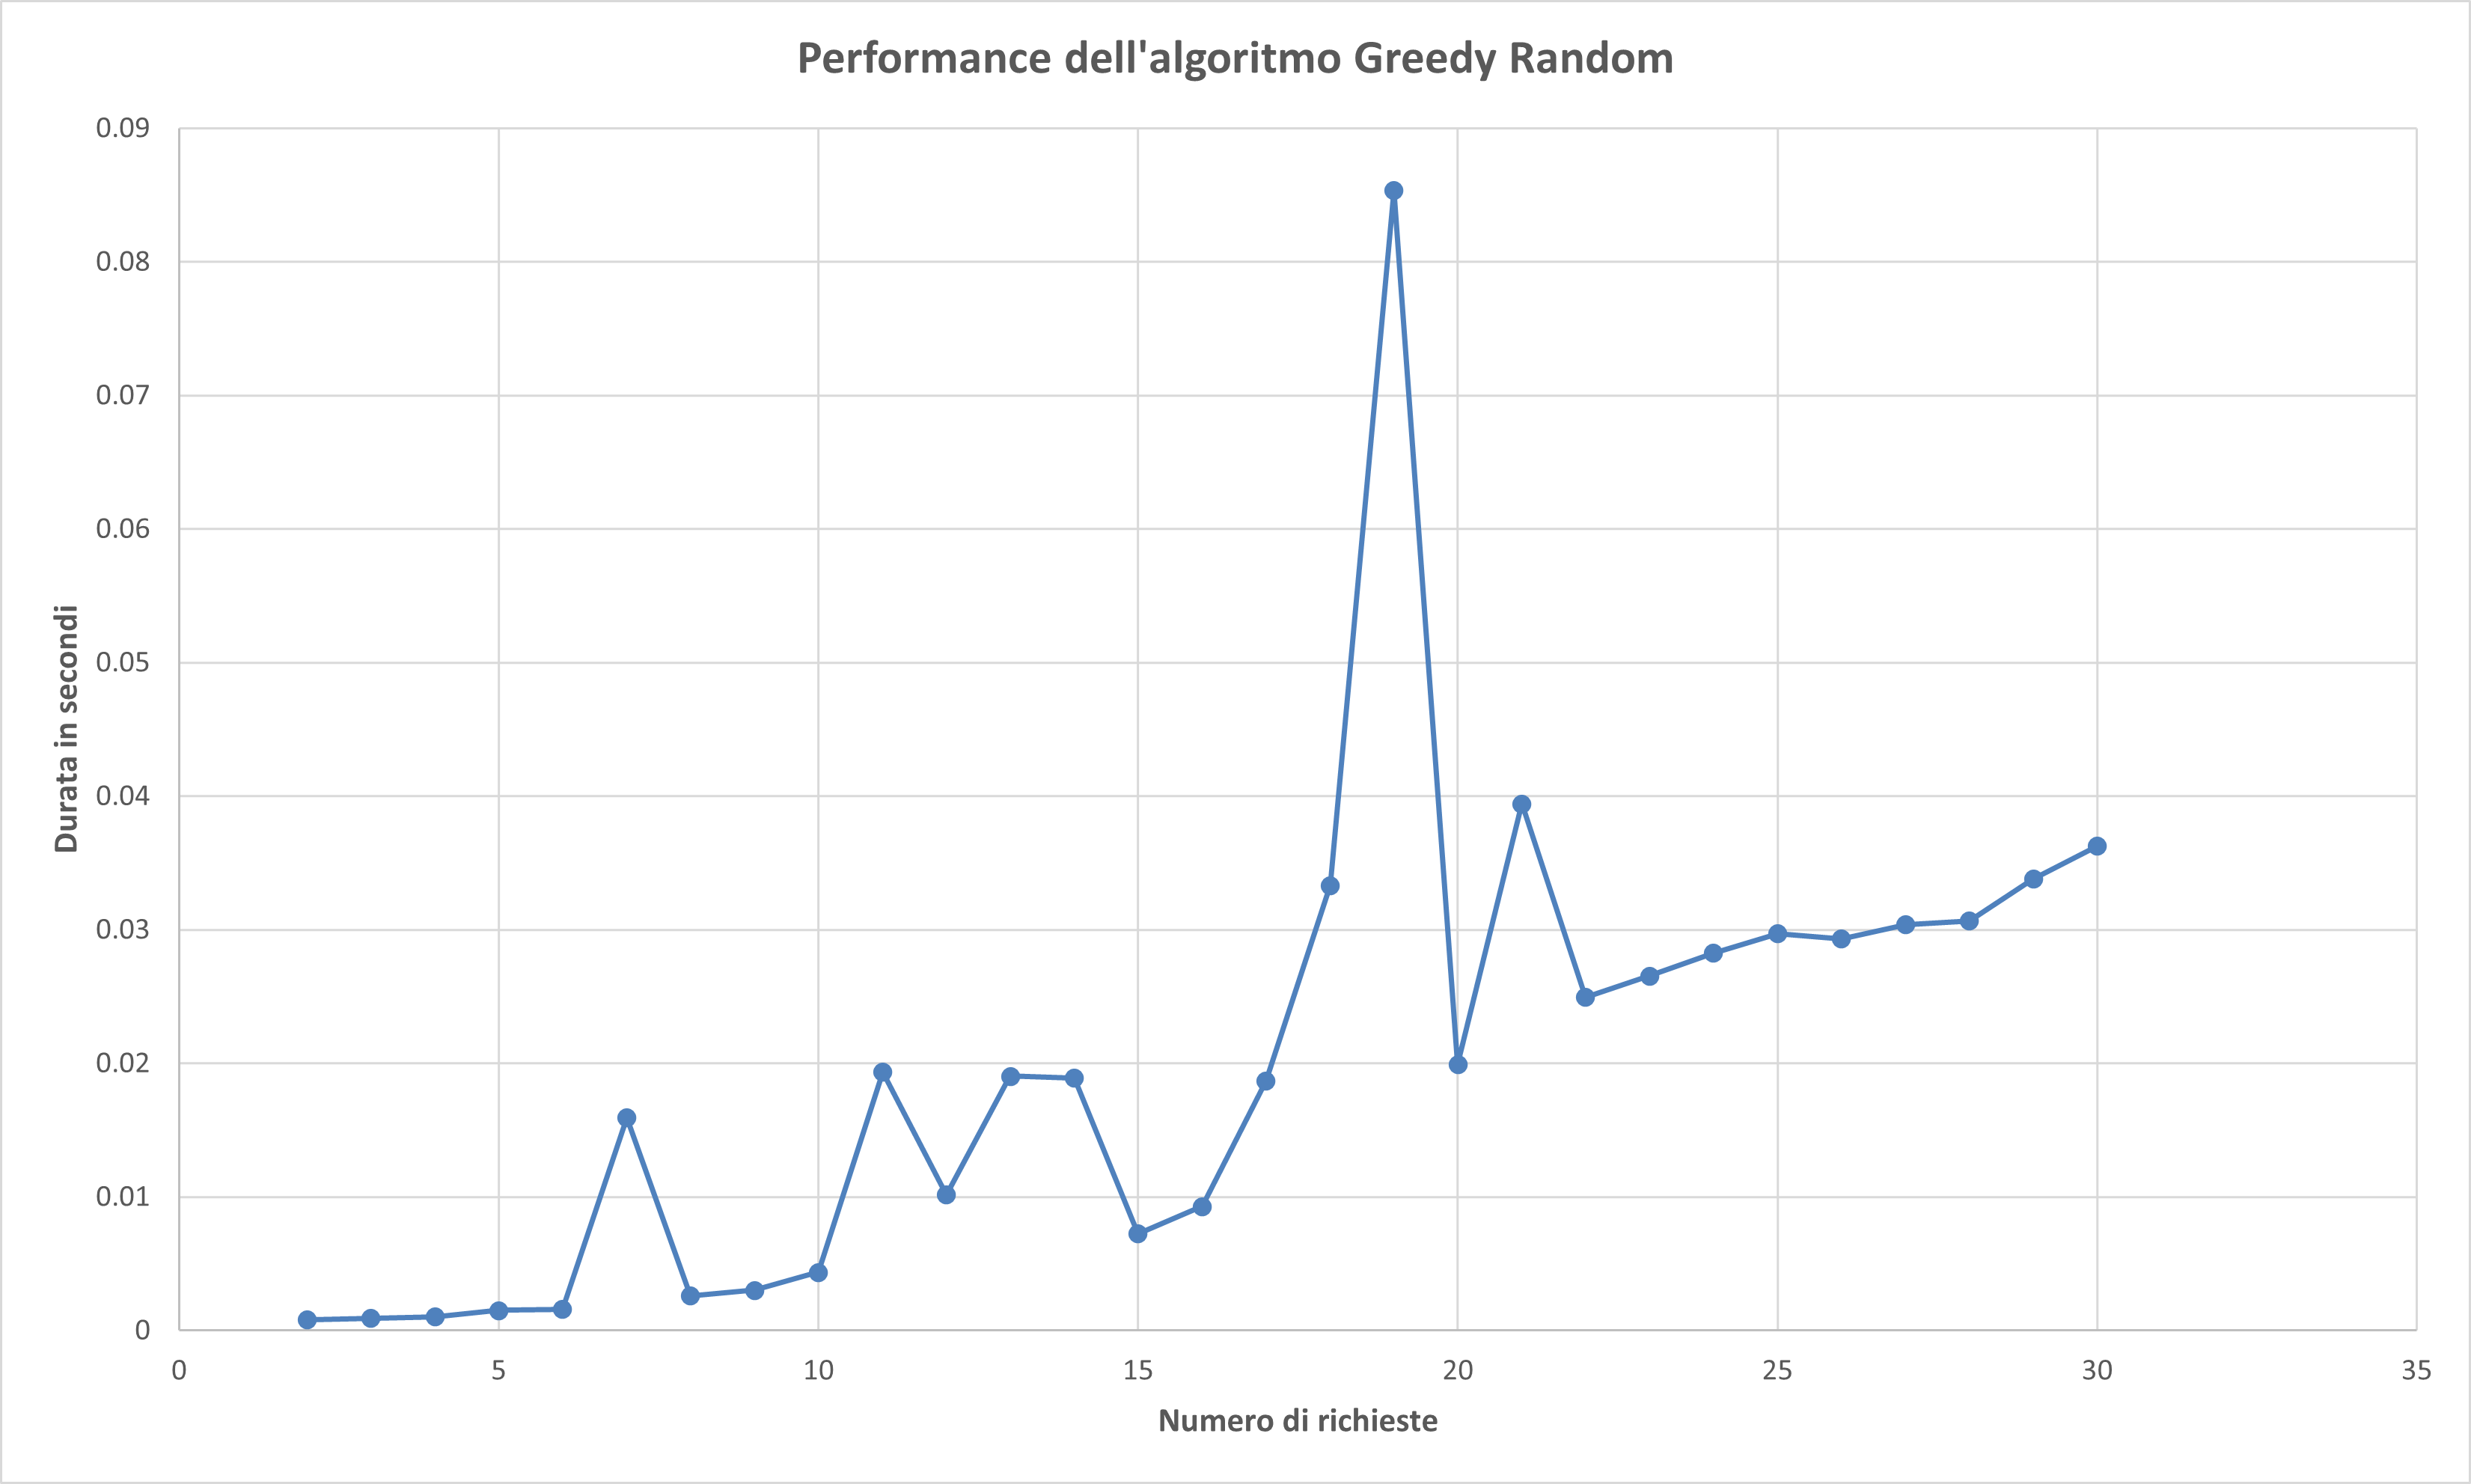
\includegraphics[width=\textwidth]
	{../charts/07 Performance dell'algoritmo Greedy Random}
	\end{figure}

\end{frame}

\subsection{Confronto}
\begin{frame}[allowframebreaks]{\subsecname}

	\textbf{Performance nel tempo}
      	\begin{figure}[h]
	\centering
	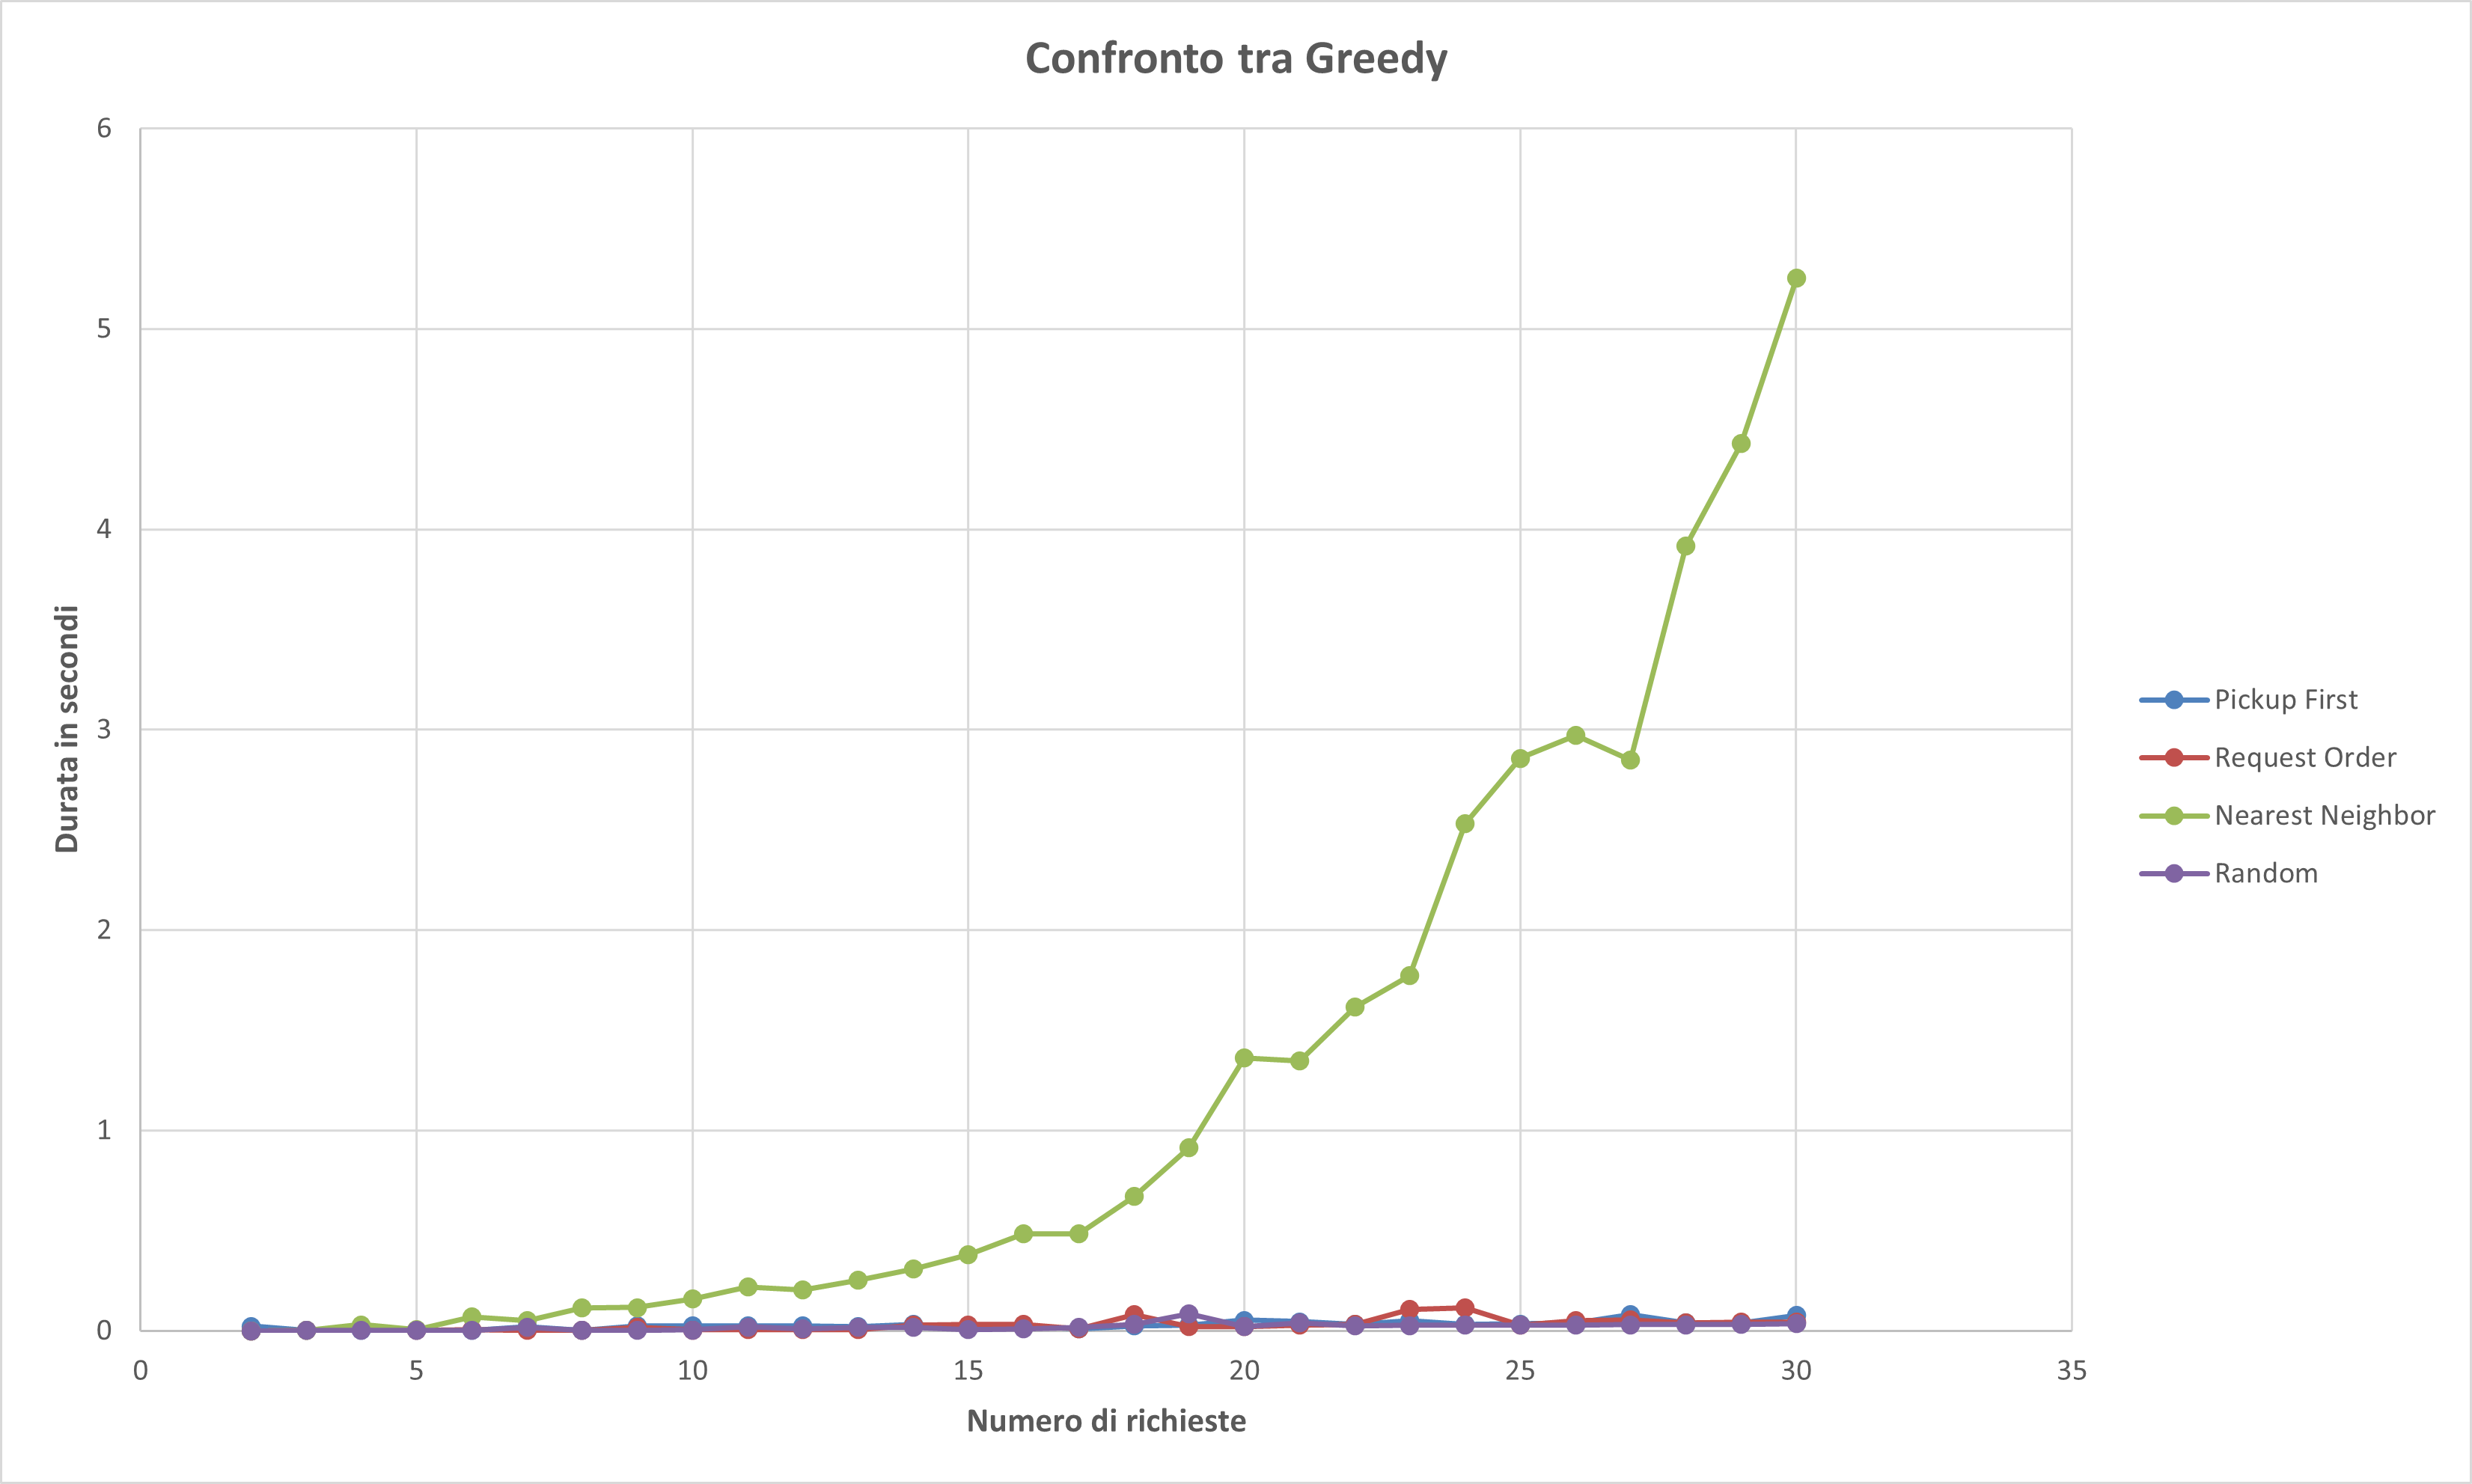
\includegraphics[width=\textwidth]
	{../charts/08a Confronto tra Greedy}
	\end{figure}

\framebreak

	\textbf{Performance costo soluzione}
      	\begin{figure}[h]
	\centering
	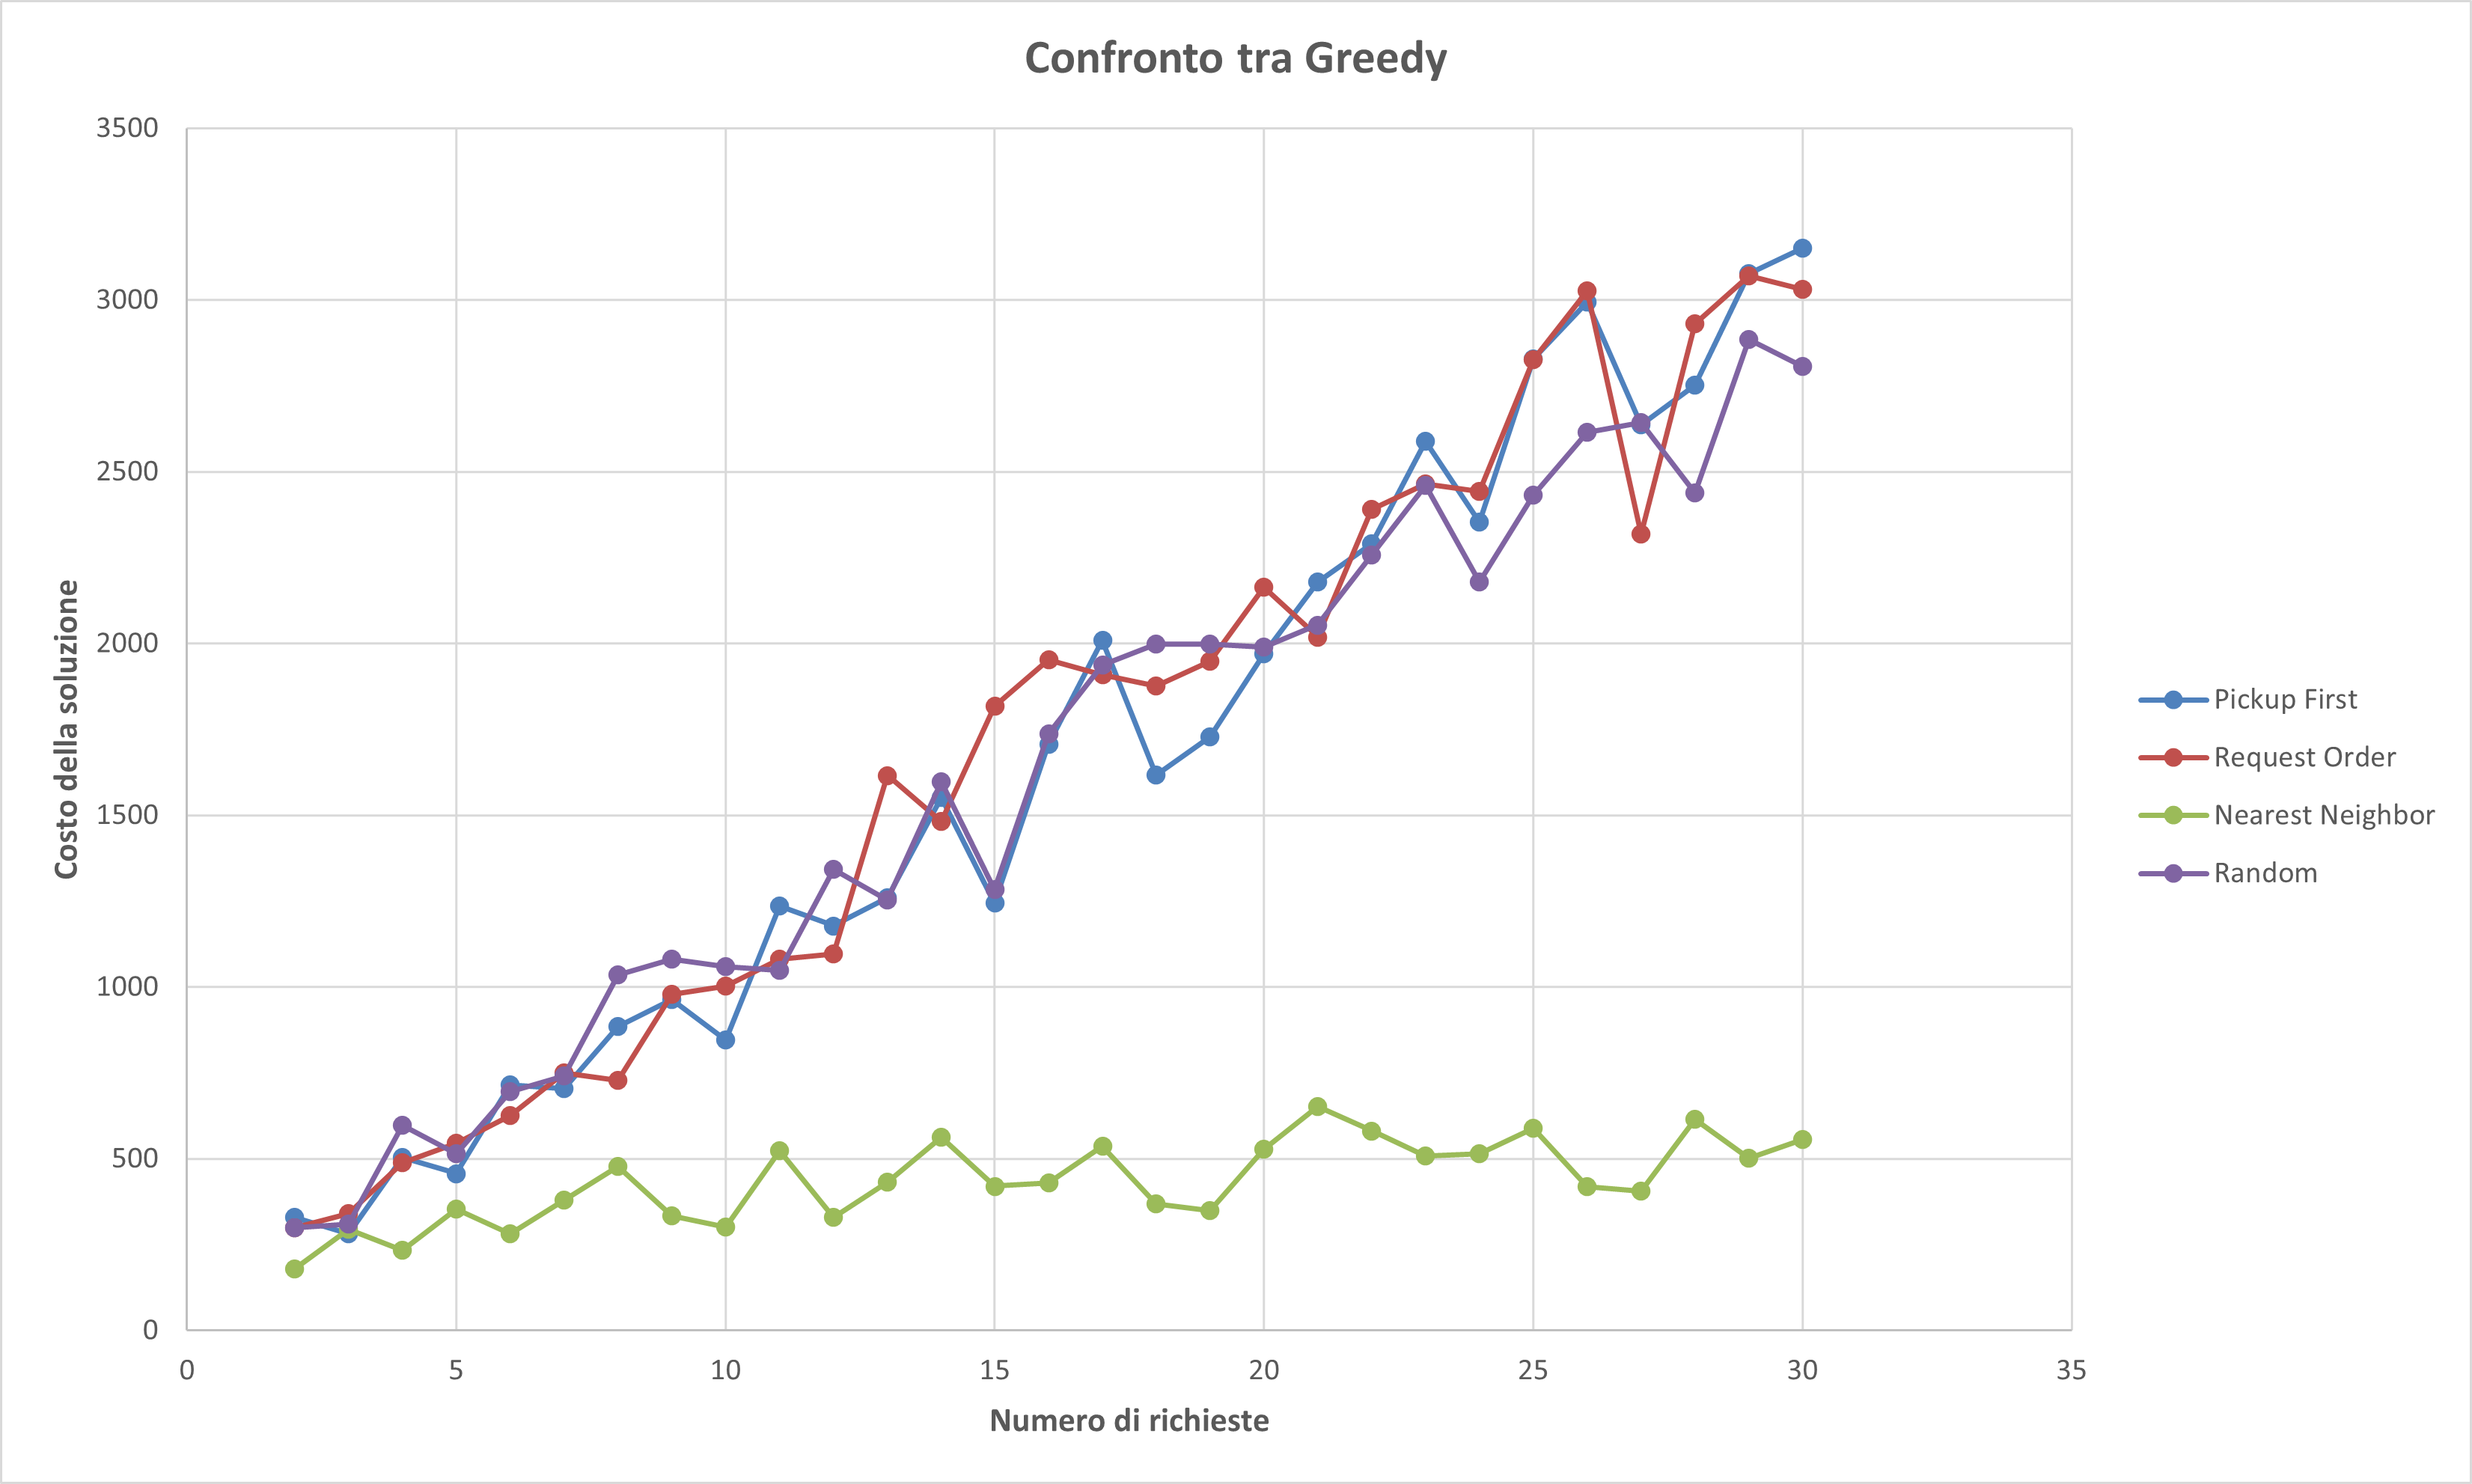
\includegraphics[width=\textwidth]
	{../charts/08b Confronto tra Greedy}
	\end{figure}

\framebreak

	\textbf{Performance errore assoluto}
      	\begin{figure}[h]
	\centering
	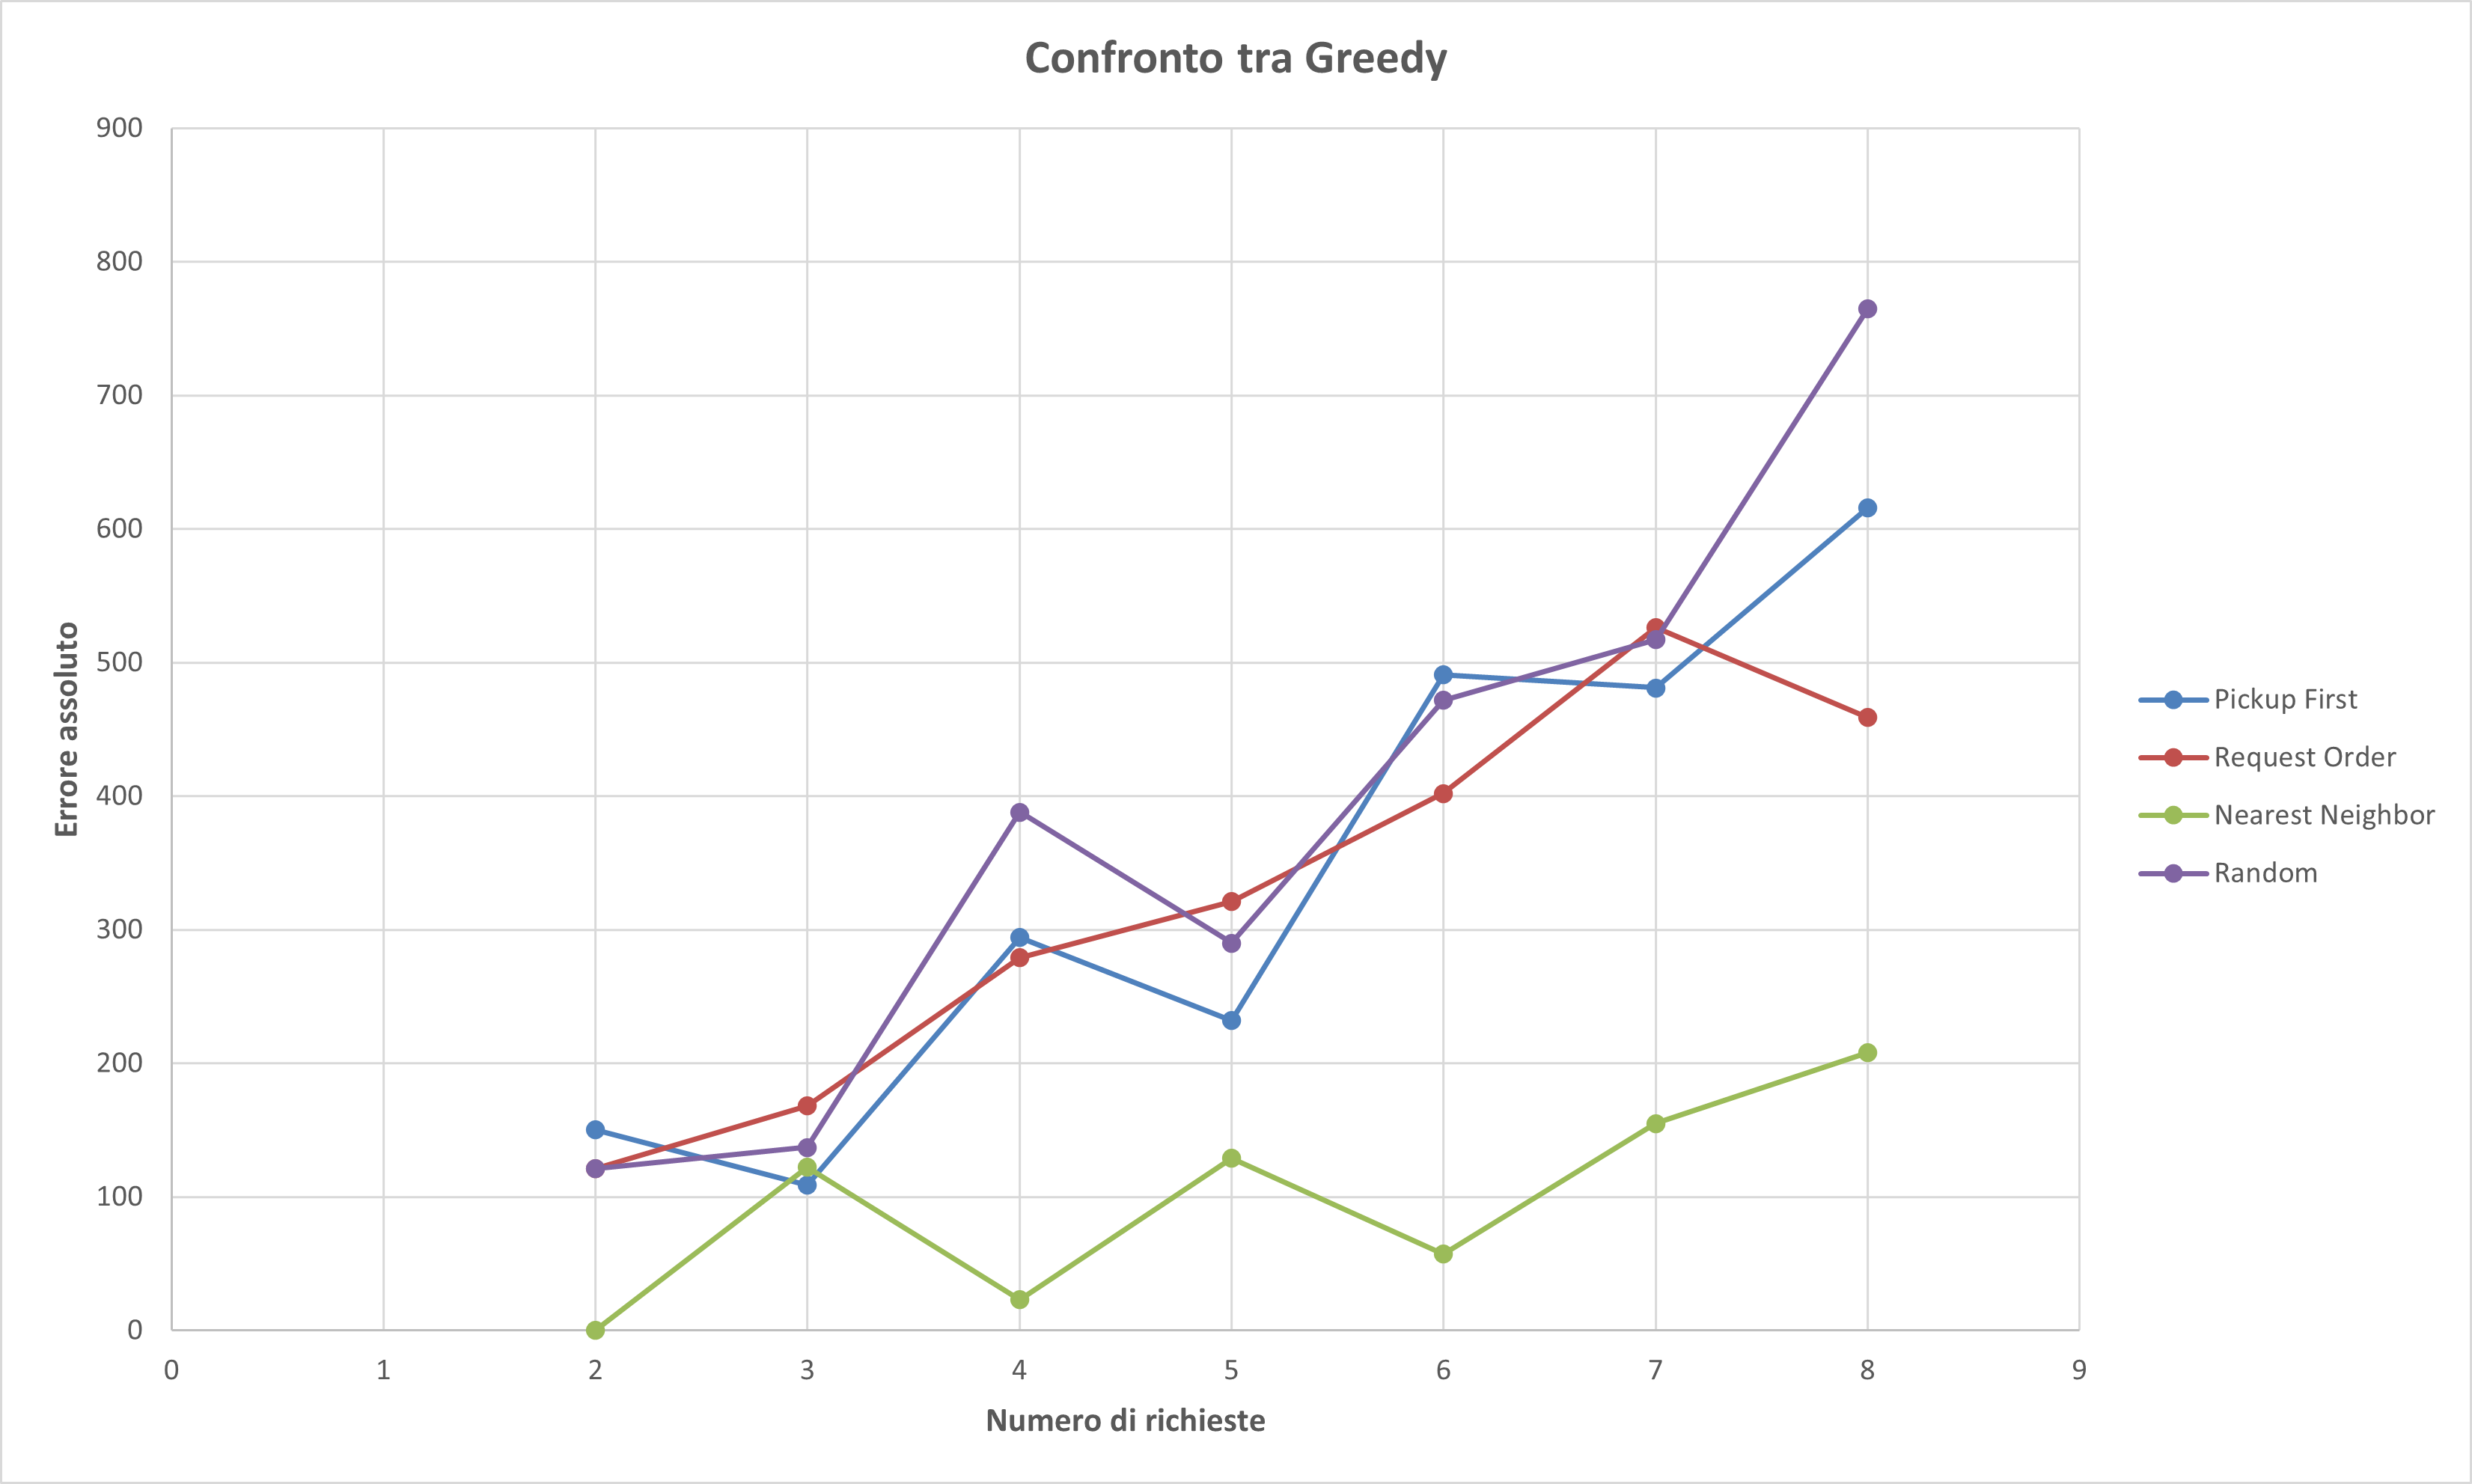
\includegraphics[width=\textwidth]
	{../charts/08c Confronto tra Greedy}
	\end{figure}

\framebreak

	\textbf{Performance errore relativo}
      	\begin{figure}[h]
	\centering
	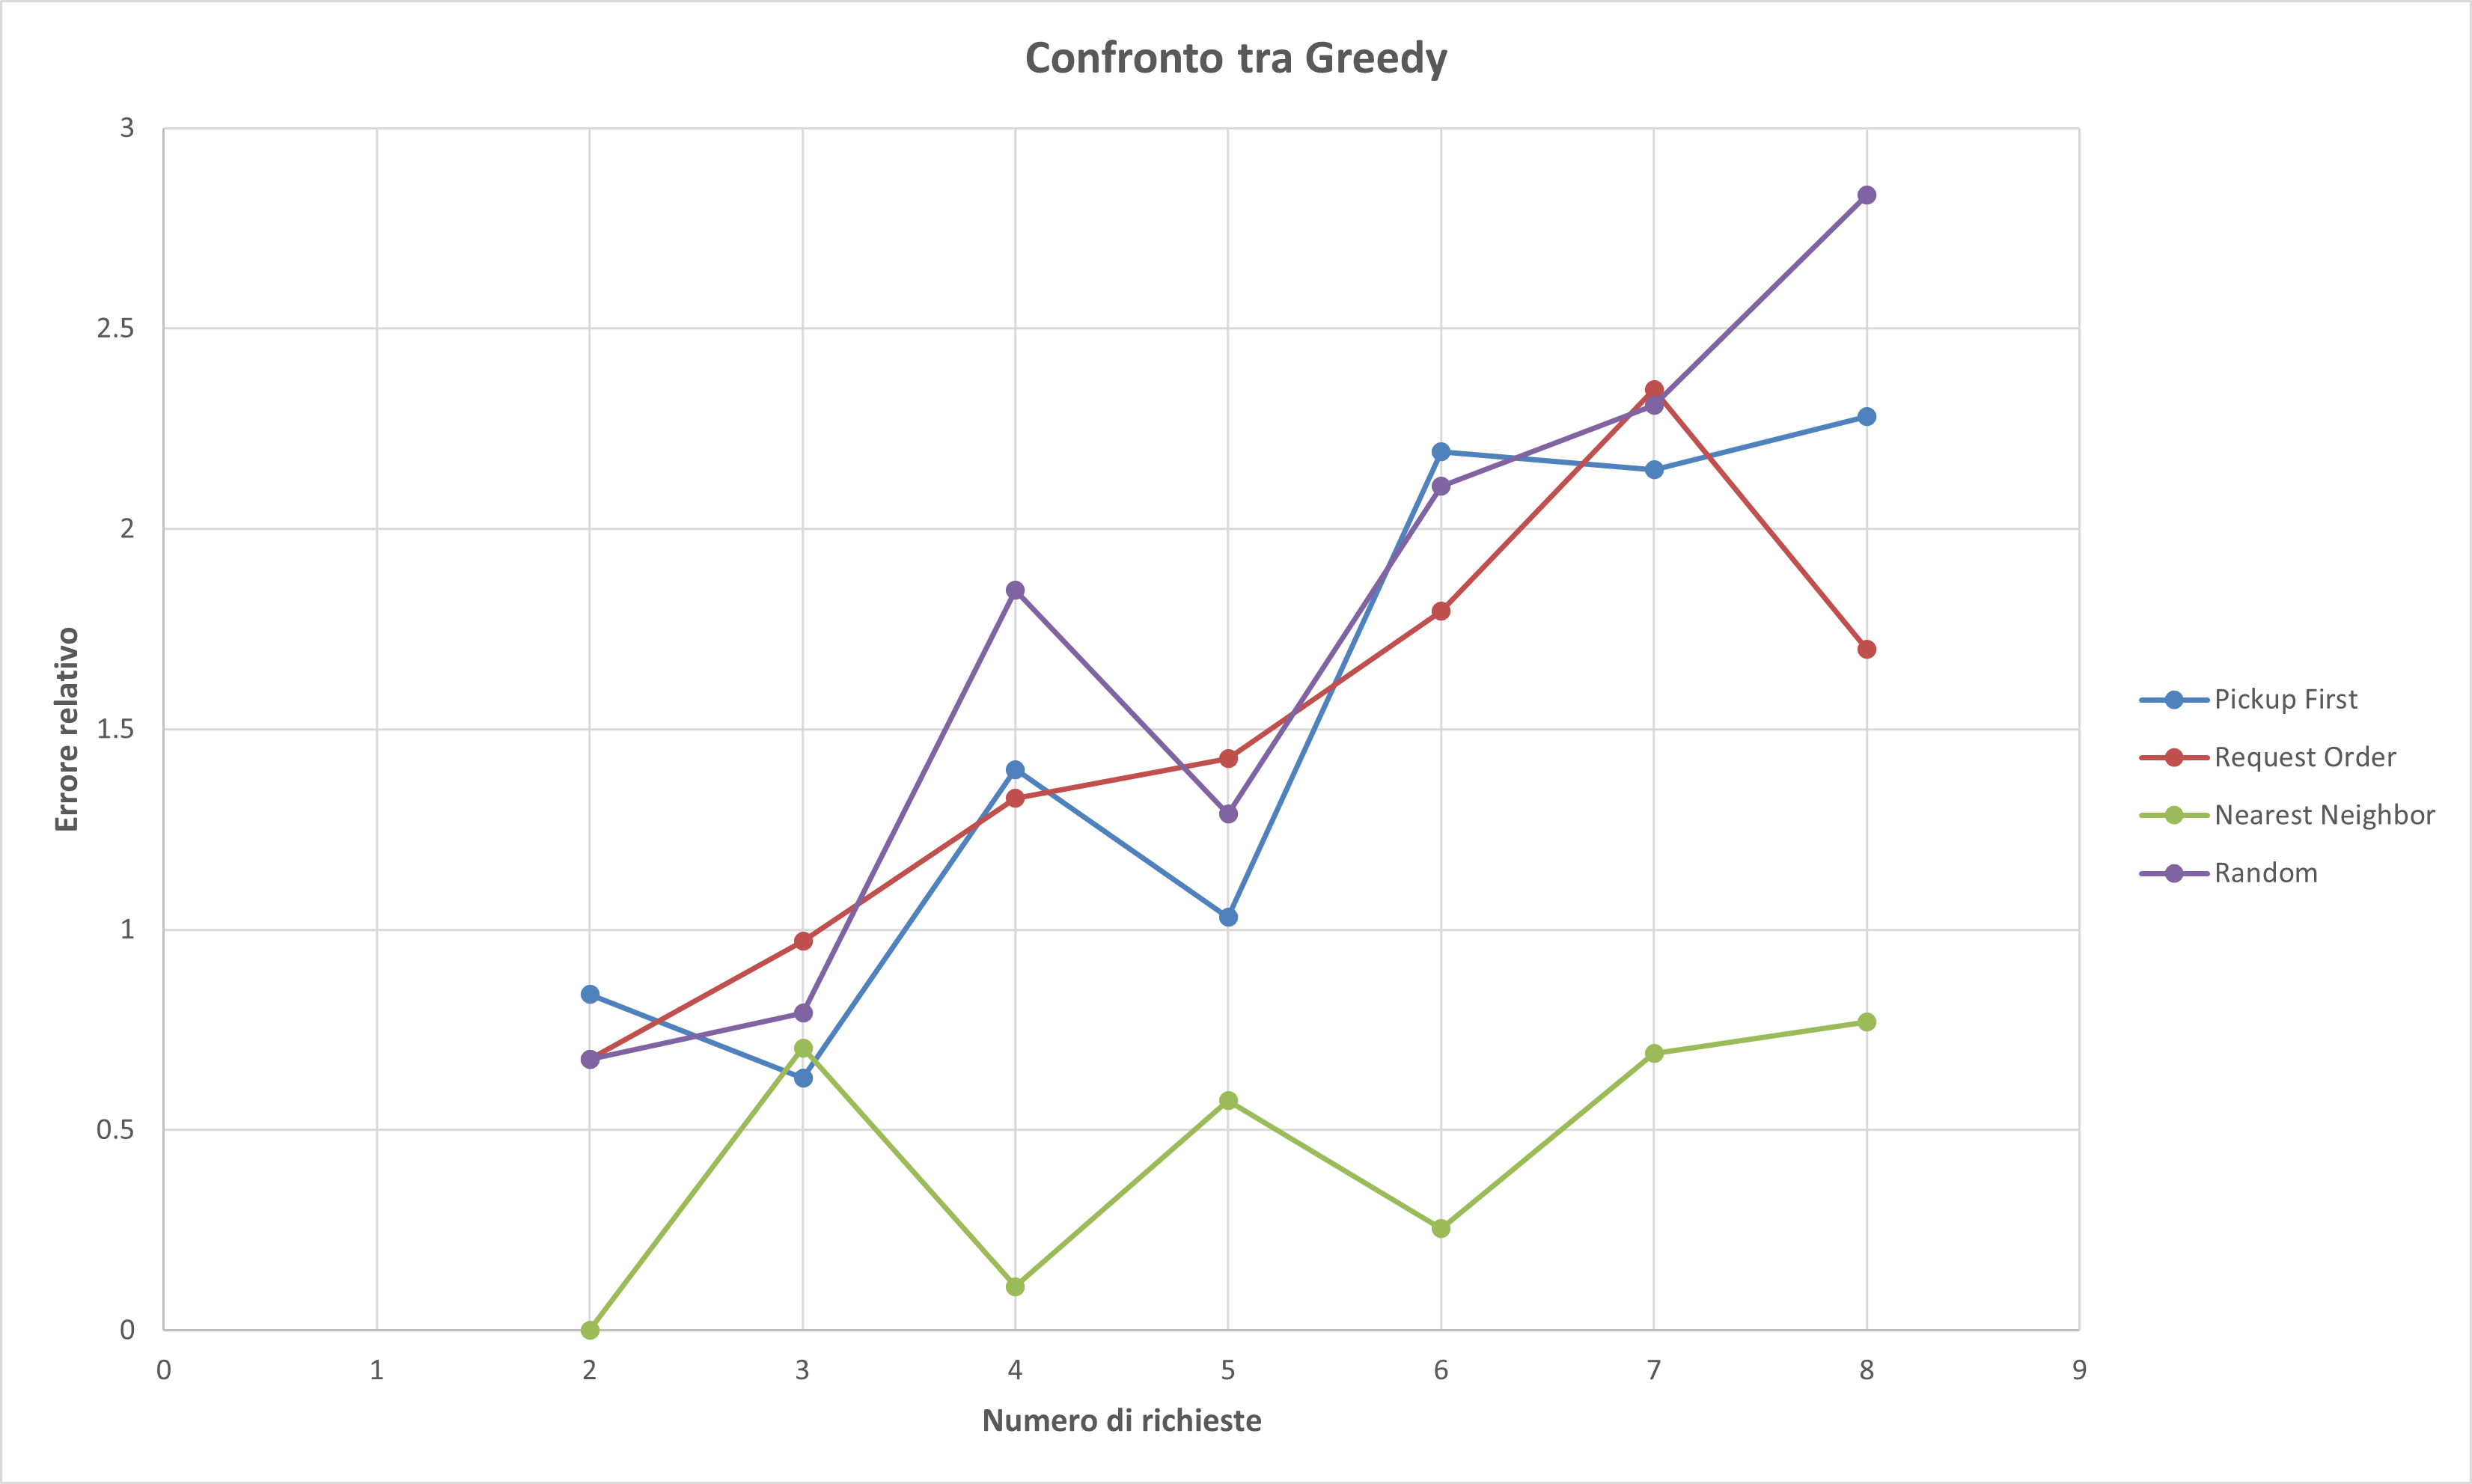
\includegraphics[width=\textwidth]
	{../charts/08d Confronto tra Greedy}
	\end{figure}

\end{frame}

%%%
%%%   ALGORITMI EURISTICI DI MIGLIORAMENTO
%%%

\section{Algoritmi euristici di miglioramento\newline
\footnotesize{Local search neighborhood based}}

\subsection{Local search neighborhood based}
\begin{frame}[allowframebreaks]{\subsecname}

	\begin{itemize}
		\item
		La ricerca locale è l’algoritmo di riferimento per tutte le (meta)euristiche basate sul concetto di intorno.
		
		\item	
		Data una soluzione $x$, l’intorno $N(x^k)$ è dato attraverso la \emph{MOSSA} che descrive operativamente cosa modifico di $x$ per generare tutte le soluzioni in $N(x^k)$.

		\item
		Se l’intorno gode della proprietà di raggiungibilità, cioè per ogni coppia di soluzioni esiste una successione di soluzioni che le collega, tale per cui ogni soluzione appartiene all’intorno della soluzione precedente, allora la ricerca è in grado di esplorare tutta la regione ammissibile $F$.

		\item
		Se esplorando l’intorno non trovo una soluzione migliore, allora vuol dire che sono in un ottimo locale per quell’intorno.
	\end{itemize}

\framebreak

	\begin{itemize}
		\item
		Esistono diverse tecniche secondo cui esplorare l’intorno. Per tutte le euristiche implementate si è scelto l’approccio \emph{best improvement}, ovvero si risolve in modo esatto il sottoproblema trovando la soluzione migliore nell’intorno.

		\item
		Come soluzione di partenza viene utilizzata la migliore delle greedy (la soluzione che ha costo più basso).

		\item
		Consultando i file exel generati durante i benchmark si può valutare anche l’approccio \emph{first improvement} (si restituisce la prima soluzione che migliora l’ottimo corrente) e \emph{h-improvement} (si restituisce la migliore delle h soluzioni che migliorano l’ottimo corrente) senza dover rieseguire i benchmark, in quanto si è memorizzato l’andamento delle migliori soluzioni durante l’esplorazione dell’intorno.
	\end{itemize}

\end{frame}

\subsection{City swap}
\begin{frame}[allowframebreaks, fragile]{\subsecname}
	\textbf{Definizione dell'algoritmo} \\
	\emph{City swap} è l’intorno ottenuto dallo scambio di 2 nodi (anzichè 2 archi) nel ciclo.

	\textbf{Codice} \\
	\href{https://github.com/michele-vaccari/TSP-con-pick-up-and-delivery/blob/main/src/tsppd/solver/citySwap.py}{https://github.com/michele-vaccari/TSP-con-pick-up-and-delivery/blob/main/src/tsppd/solver/citySwap.py}

	\textbf{Esempio}
	\begin{figure}[h]
	\centering
	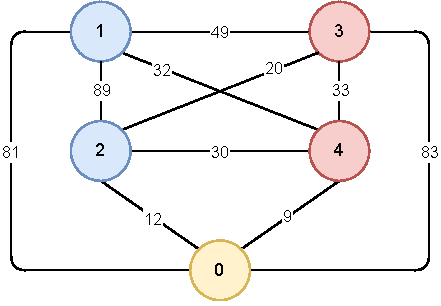
\includegraphics[width=0.35\textwidth]
	{../images/graph-tsppd-with-two-customers}	
	\caption{Istanza iniziale}
	\end{figure}

\framebreak
	{\footnotesize
	\textbf{Esecuzione} \\
	La soluzione di partenza è la migliore delle greedy $\rightarrow s_0 = [0,1,3,2,4] \quad c(s_0) = 189$

	\textbf{Passi dell’algoritmo:}
	\begin{enumerate}
		\item
		Scambio il $3$ con il $2 \rightarrow s_1 = [0,1,2,3,4,0] \quad c(s_1) = 232$

		\item
		\label{city-swap-case}
		Scambio il $2$ con il $3 \rightarrow s_2 = [0,1,2,3,4,0] \quad c(s_2) = 232$
	\end{enumerate}
	\textbf{N.B.} La tabu search mi impedirebbe il punto \ref{city-swap-case}

	\captionsetup{justification=centering,font=footnotesize}

      \begin{columns}[T,onlytextwidth]
		\column{0.33\textwidth}
		\begin{figure}[h]
		\centering
		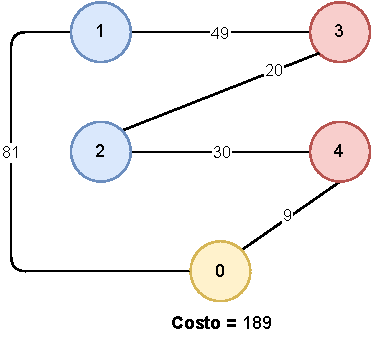
\includegraphics[height=0.25\textheight]
		{../images/graph-greedy-request-order-solution-tsppd-with-two-customers}	
		\caption{Soluzione $s_0$}
		\end{figure}
		\column{0.33\textwidth}
		\begin{figure}[h]
		\centering
		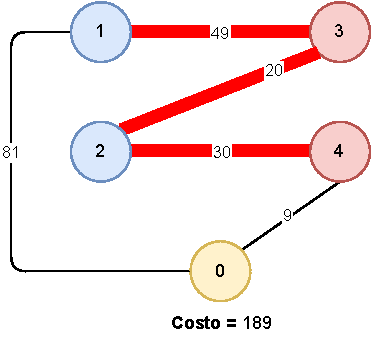
\includegraphics[height=0.25\textheight]
		{../images/city-swap}	
		\caption{Archi eliminati al passo \ref{city-swap-case}}
		\end{figure}
		\column{0.33\textwidth}
		\begin{figure}[h]
		\centering
		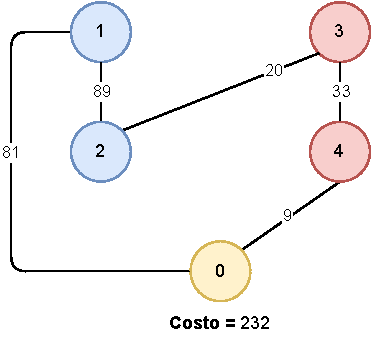
\includegraphics[height=0.25\textheight]
		{../images/graph-greedy-pickup-first-solution-tsppd-with-two-customers}	
		\caption{Soluzione $s_1$}
		\end{figure}
	\end{columns}

	Il passo \ref{city-swap-case} è un 2 opt limitato agli archi incidenti su questi nodi
	}
\framebreak

	\textbf{Performance nel tempo}
      	\begin{figure}[h]
	\centering
	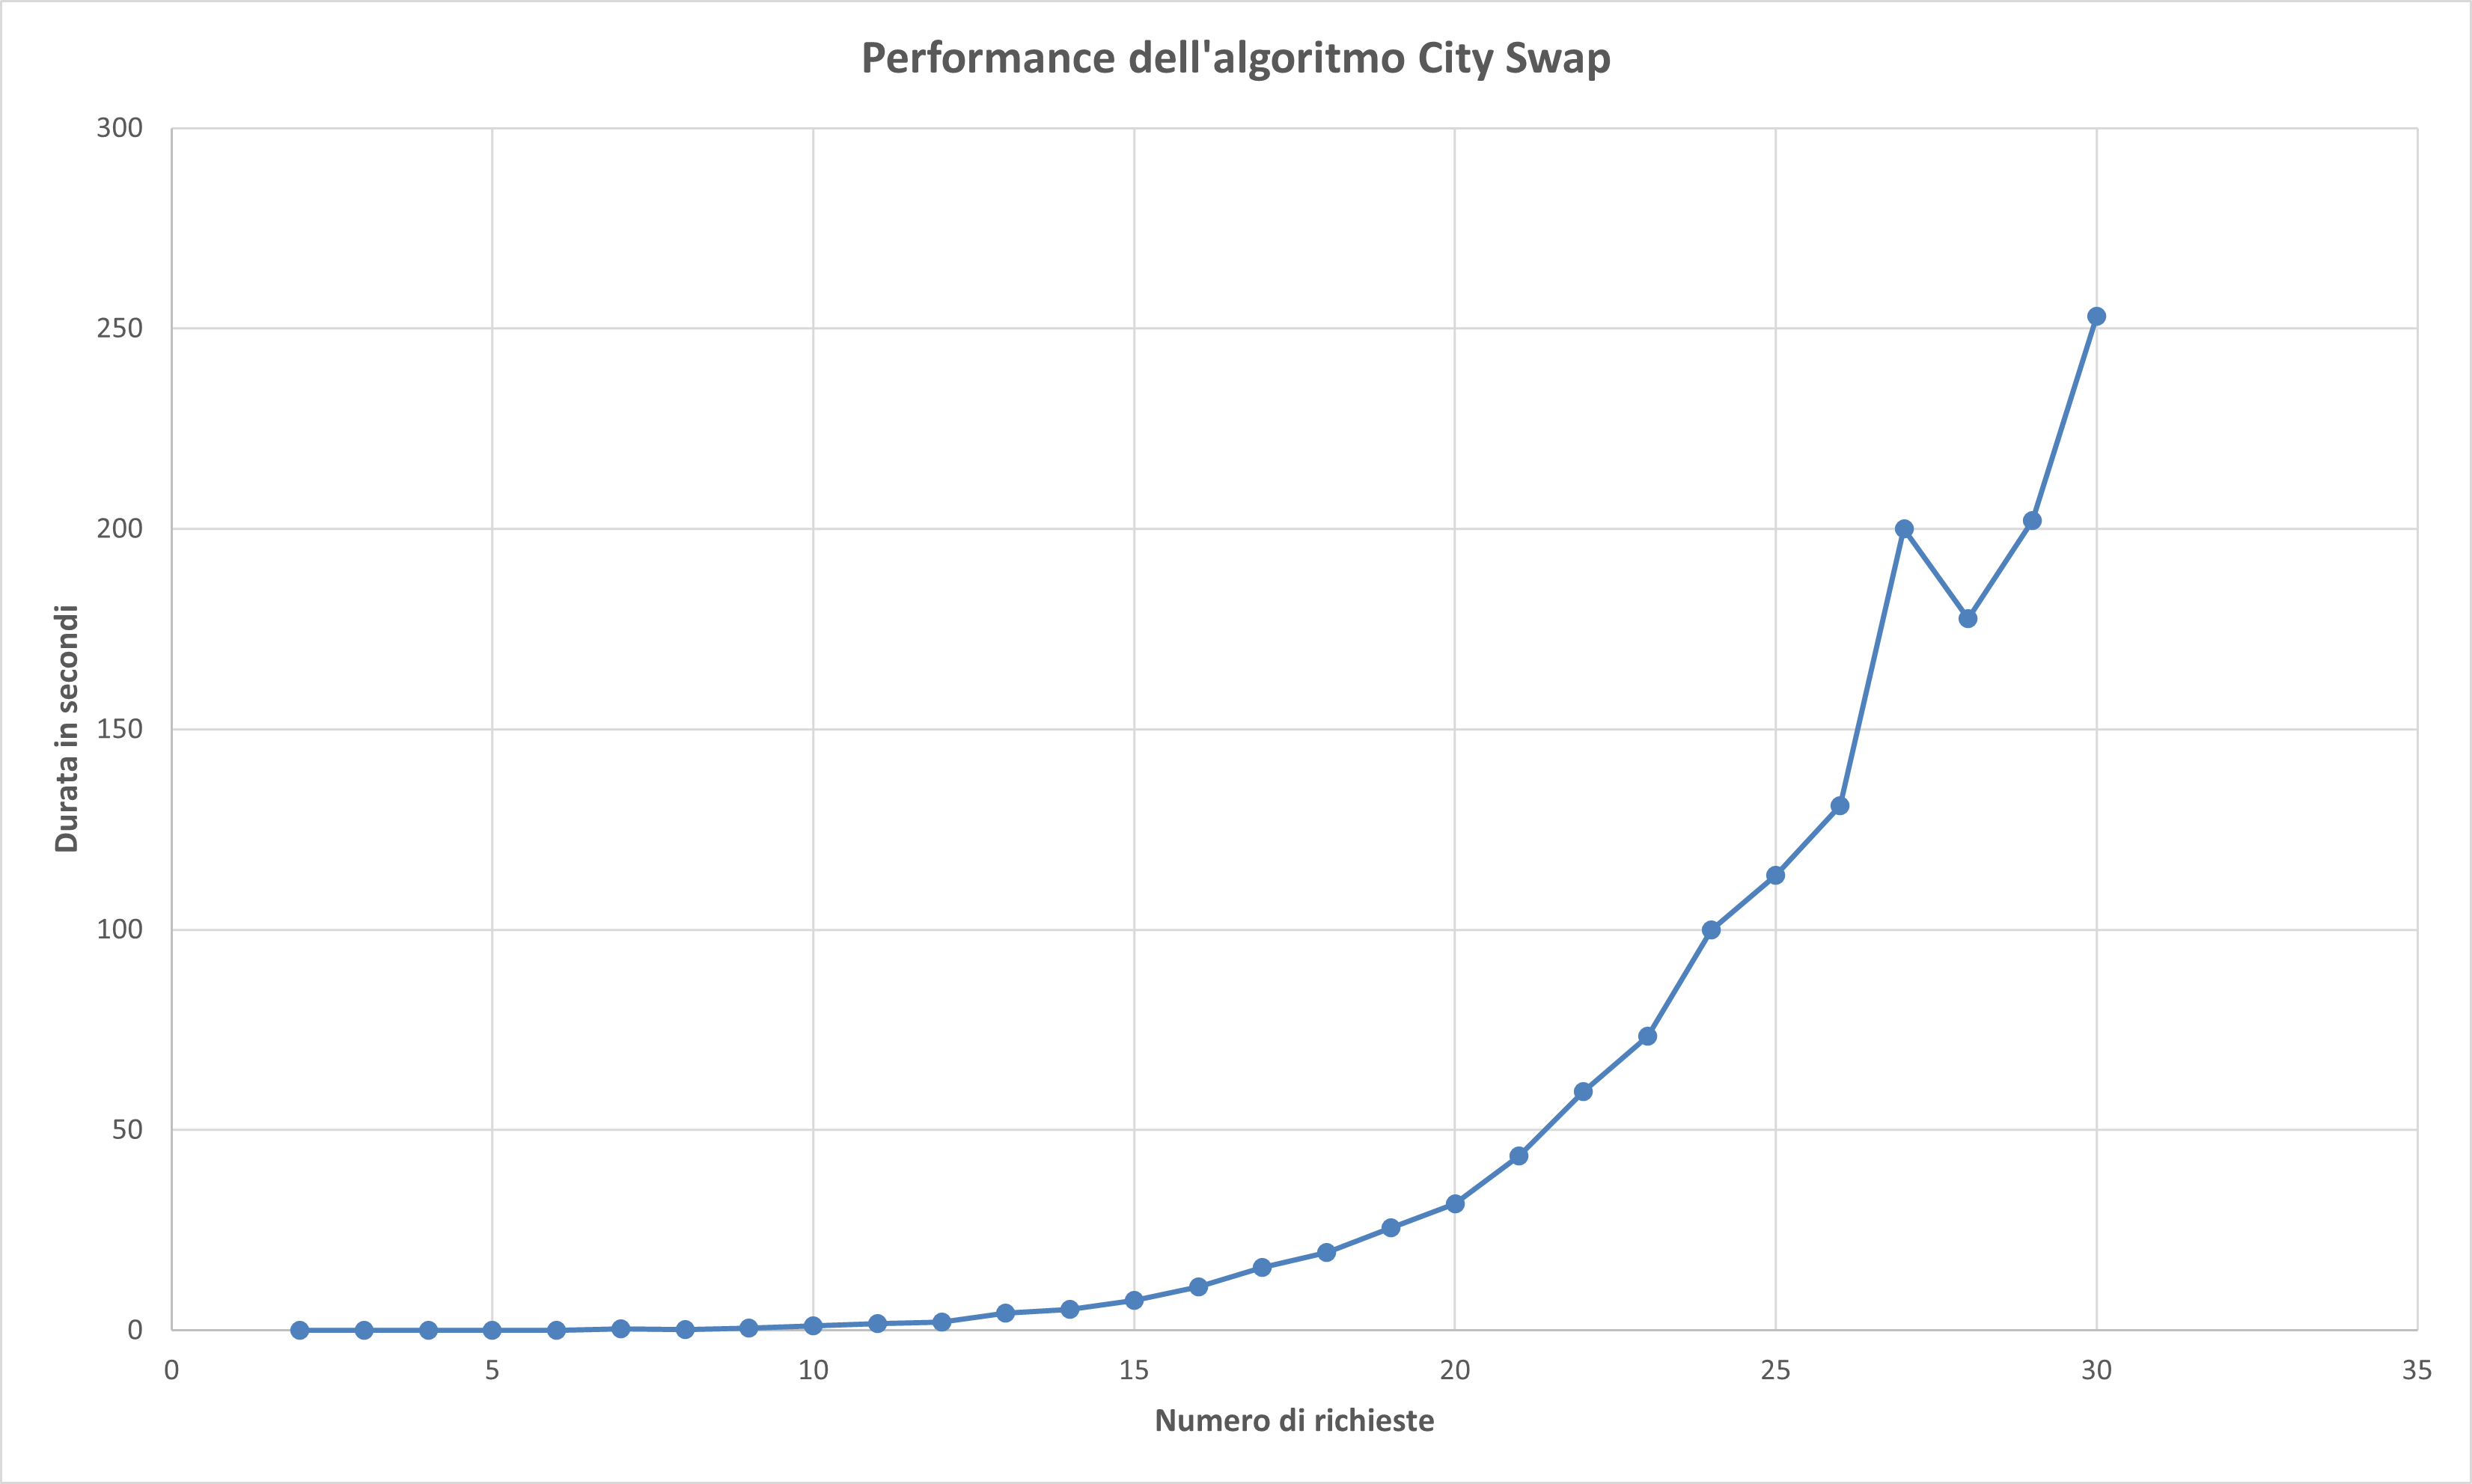
\includegraphics[width=\textwidth]
	{../charts/10 Performance dell'algoritmo City Swap}
	\end{figure}

\end{frame}

\subsection{City insert}
\begin{frame}[allowframebreaks]{\subsecname}
	\textbf{Definizione dell'algoritmo} \\
	\emph{City insert} è l’intorno ottenuto dalla cancellazione di 1 nodo nel ciclo e dal suo reinserimento in un altro punto.

	\textbf{Codice} \\
	\href{https://github.com/michele-vaccari/TSP-con-pick-up-and-delivery/blob/main/src/tsppd/solver/citySwap.py}{https://github.com/michele-vaccari/TSP-con-pick-up-and-delivery/blob/main/src/tsppd/solver/citySwap.py}

	\textbf{Esempio}
	\begin{figure}[h]
	\centering
	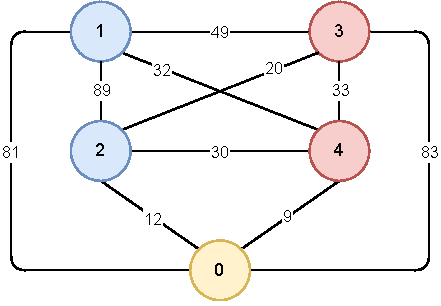
\includegraphics[width=0.35\textwidth]
	{../images/graph-tsppd-with-two-customers}	
	\caption{Istanza iniziale}
	\end{figure}

\framebreak
	{\footnotesize
	\textbf{Esecuzione} \\
	La soluzione di partenza è la migliore delle greedy $\rightarrow s_0 = [0,1,3,2,4] \quad c(s_0) = 189$

	\textbf{Passi dell’algoritmo:}
	\begin{enumerate}
		\item
		\label{city-insert-case}
		Cancello il $3$ e lo reinserisco dopo il $2 \rightarrow s_1 = [0,1,2,3,4] \quad c(s_1) = 232$
		\item
		Cancello il $3$ e lo reinserisco dopo il $4 \rightarrow s_2 = [0,1,2,4,3] \quad c(s_2) = 316$
		\item
		Cancello l’$1$ e lo reinserisco dopo il $2 \rightarrow s_3 = [0,2,1,3,4] \quad c(s_3) = 192$
		\item
		Cancello il $2$ e lo reiserisco dopo l’$1 \rightarrow s_4 = [0,1,2,3,4] \quad c(s_4) = 232$
	\end{enumerate}

	\captionsetup{justification=centering,font=footnotesize}

      \begin{columns}[T,onlytextwidth]
		\column{0.33\textwidth}
		\begin{figure}[h]
		\centering
		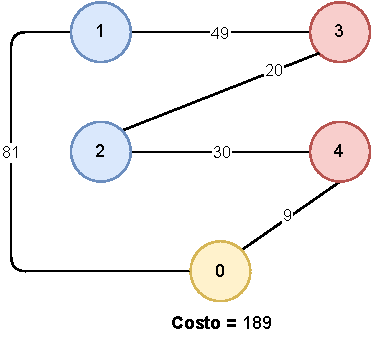
\includegraphics[height=0.25\textheight]
		{../images/graph-greedy-request-order-solution-tsppd-with-two-customers}	
		\caption{Soluzione $s_0$}
		\end{figure}
		\column{0.33\textwidth}
		\begin{figure}[h]
		\centering
		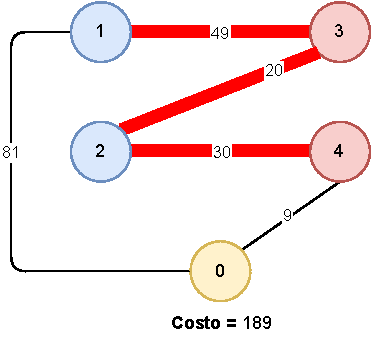
\includegraphics[height=0.25\textheight]
		{../images/city-swap}	
		\caption{Archi eliminati al passo \ref{city-insert-case}}
		\end{figure}
		\column{0.33\textwidth}
		\begin{figure}[h]
		\centering
		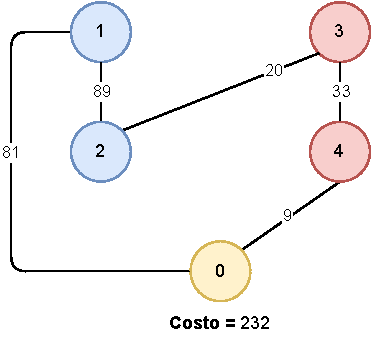
\includegraphics[height=0.25\textheight]
		{../images/graph-greedy-pickup-first-solution-tsppd-with-two-customers}	
		\caption{Soluzione $s_1$}
		\end{figure}
	\end{columns}

	Il passo \ref{city-insert-case} è un 2 opt limitato agli archi incidenti su questi nodi}
	
\framebreak

	\textbf{Performance nel tempo}
      	\begin{figure}[h]
	\centering
	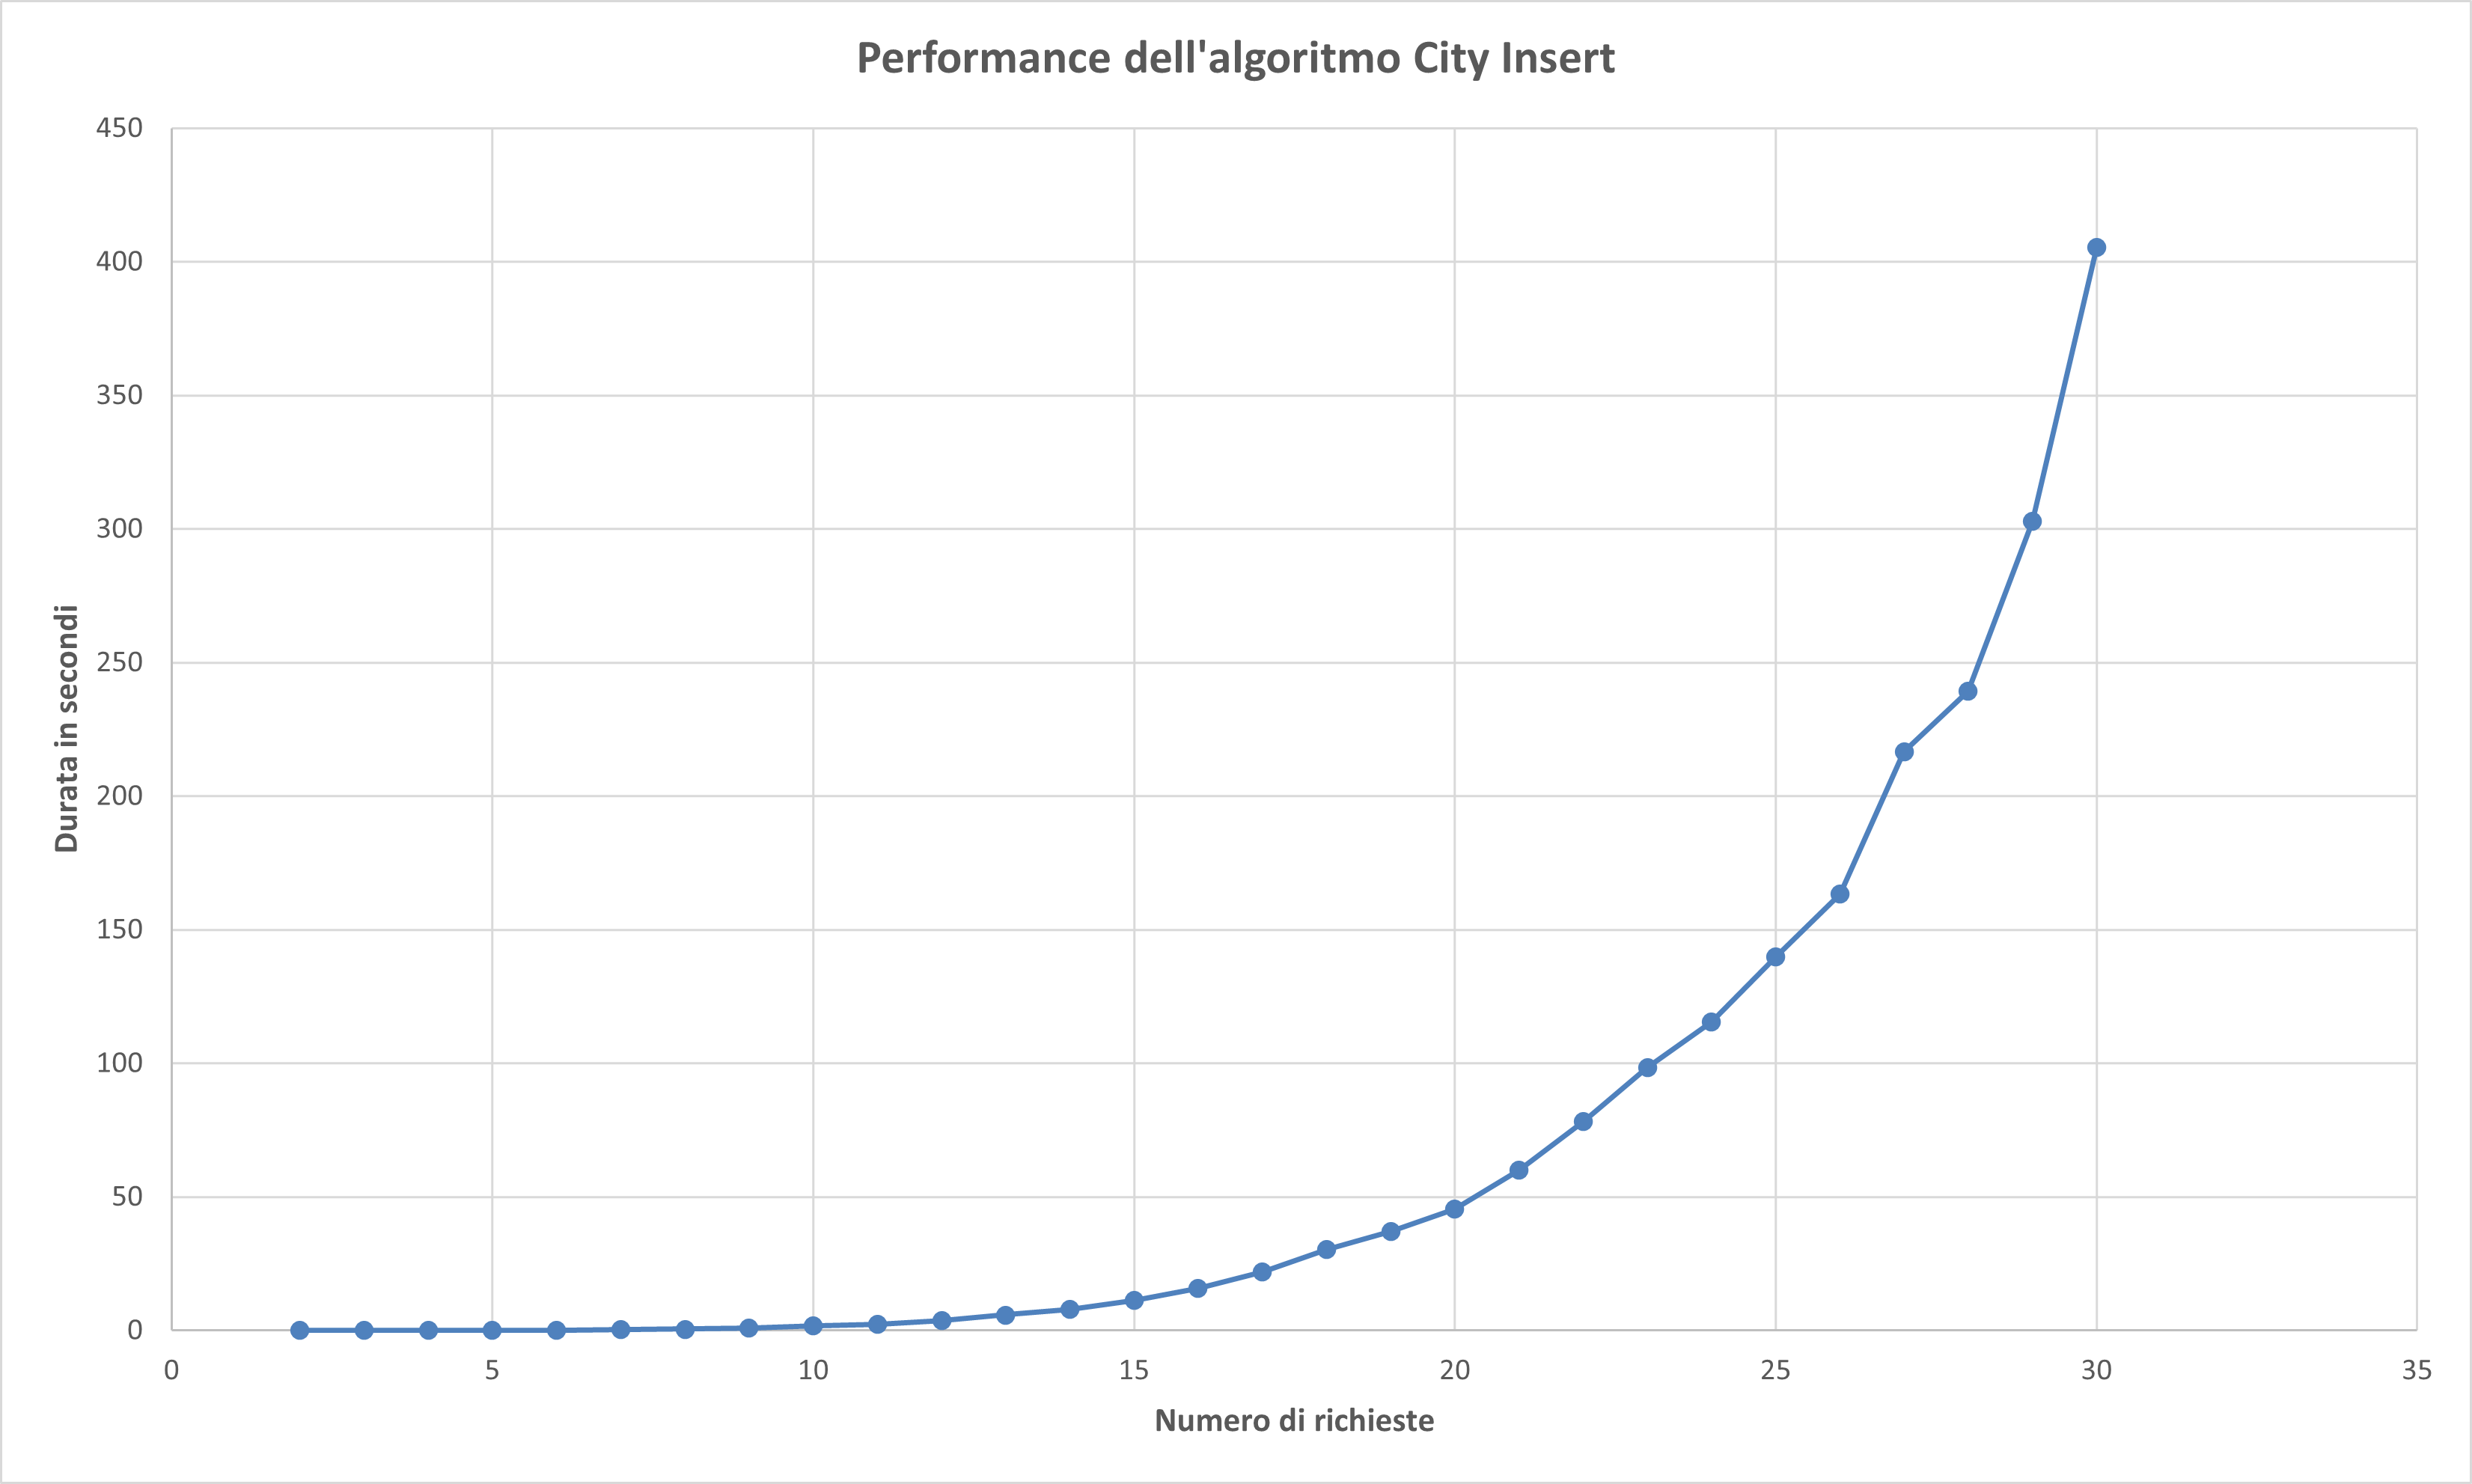
\includegraphics[width=\textwidth]
	{../charts/09 Performance dell'algoritmo City Insert}
	\end{figure}

\end{frame}

\subsection{Osservazioni}
\begin{frame}{\subsecname}

	\begin{itemize}
	
		\item
		Gli algoritmi Node-based Neighborhood City Swap e City Insert portano ad un ottimo locale

		\item
		Ad ogni iterazione si tratta di risolvere un problema di ottimizzazione. Quindi la procedura restituisce, nel caso di best improvement, la migliore soluzione dell’intorno

		\item
		Resta intrappolata negli ottimi locali

		\item
		La soluzione prodotta è determinata dalla scelta dell’intorno, dalla strategia di esplorazione e dal punto iniziale, che determina come risultato l’ottimo locale del bacino di attrazione su cui è posizionato il punto iniziale (se si segue una strategia best improvement)
		
	\end{itemize}

\end{frame}

\section{Algoritmi euristici di miglioramento\newline
\footnotesize{Oltre la local search}}

\subsection{Oltre la Local Search}
\begin{frame}{\subsecname}
	
	Per uscire dal bacino di attrazione degli ottimi locali si devono accettare anche dei peggioramenti. \\
	Per evitare di tornare su soluzioni già visitate e andare in loop è possibile:
	\begin{itemize}
		\item
		Accettare peggioramenti con probabilità decrescente (Simulated Annealing)
		\item
		Memorizzare le $N$ ultime mosse eseguite (Tabu Search)
		\item
		Allargare la visione strettamente locale della local search
	\end{itemize}

\end{frame}

%%%
%%%   SIMULATED ANNEALING
%%%
\subsection{Simulated Annealing}
\begin{frame}[allowframebreaks, fragile]{\subsecname}

	Annealing è il processo di raffreddamento secondo cui un solido raggiunge uno stato di energia minima che gli conferisce stabilità. \\
	Il metodo converge all’ottimo globale con opportuni parametri.

	\textbf{Descrizione dell'algoritmo} \\
	Ad ogni iterazione una soluzione è scelta a caso dall’intorno della soluzione corrente: l’intorno non viene esplorato, bensì campionato. \\
	Se la mossa applicata alla soluzione porta ad un miglioramento, viene sempre accettata. \\
	Altrimenti, la decisione se spostarsi ad una soluzione peggiore dipende da una funzione casuale $e^{-\Delta / T}$ dove:
	\begin{itemize}
		\item
		$\Delta = costo(sol_{ottenuta\,dal\,campionamento\,dell'intorno}) - costo(sol_{migliore\,corrente})$
		\item
		$T$ = parametro temperatura che diminuisce durante l'euristica
	\end{itemize}

\framebreak

	\textbf{Parametri utilizzati nell'algoritmo}
	\begin{itemize}
		\item
		Soluzione iniziale: la migliore soluzione ottenuta dalle greedy
		\item
		Intorno utilizzato: city swap
		\item
		Temperatura iniziale: 900
		\item
		Tasso di raffreddamento: 0.92
		\item
		Temperatura finale: 0.1
		\item
		Iterazioni per temperatura: 5
	\end{itemize}

	\textbf{Codice} \\
	\href{https://github.com/michele-vaccari/TSP-con-pick-up-and-delivery/blob/main/src/tsppd/solver/simulatedAnnealing.py}{https://github.com/michele-vaccari/TSP-con-pick-up-and-delivery/blob/main/src/tsppd/solver/simulatedAnnealing.py}

\framebreak

	\textbf{Schema dell'algoritmo}
\begin{minted}[fontsize=\scriptsize, escapeinside=;;, tabsize=2]{c}
Simulated Annealing(problem) return a solution

	;$T \leftarrow determine\,a\,starting\,temperature$;
	;$current \leftarrow generate\,an\,initial\,solution$;
	;$best \leftarrow current$;
	while ;$(not\,yet\,frozen)$; do // finchè ;$T > T_{frozen}$;
		while ;$not\,yet\,at\,equilibrium\,for\,this\,temperature$; do
			;$next \leftarrow a\,random\,solution\,selected\,from\,Neighbor(current)$;
			;$\Delta E \leftarrow f(next) - f(current)$;
			if ;$\Delta E < 0 $; then ;$current \leftarrow next $; // miglioramento
				if ;$f(next) < f(best)$; then ;$best \leftarrow next$; // aggiorno best
			else
				;$choose\,a\,random\,number\,r\,uniformly\,in\,[0,1]$;
				if ;$r < e^{-\Delta E / T} $; then ;$current \leftarrow next $; // accetta peggioramento con prob ;$ e^{-\Delta E / T} > 0 $;
		end while
		;$lower\,the\,temperature\,T$; // equilibrio raggiunto per T
	end while // processo di raffreddamento terminato
	return best
\end{minted}

\framebreak
	\textbf{Performance nel tempo}
      	\begin{figure}[h]
	\centering
	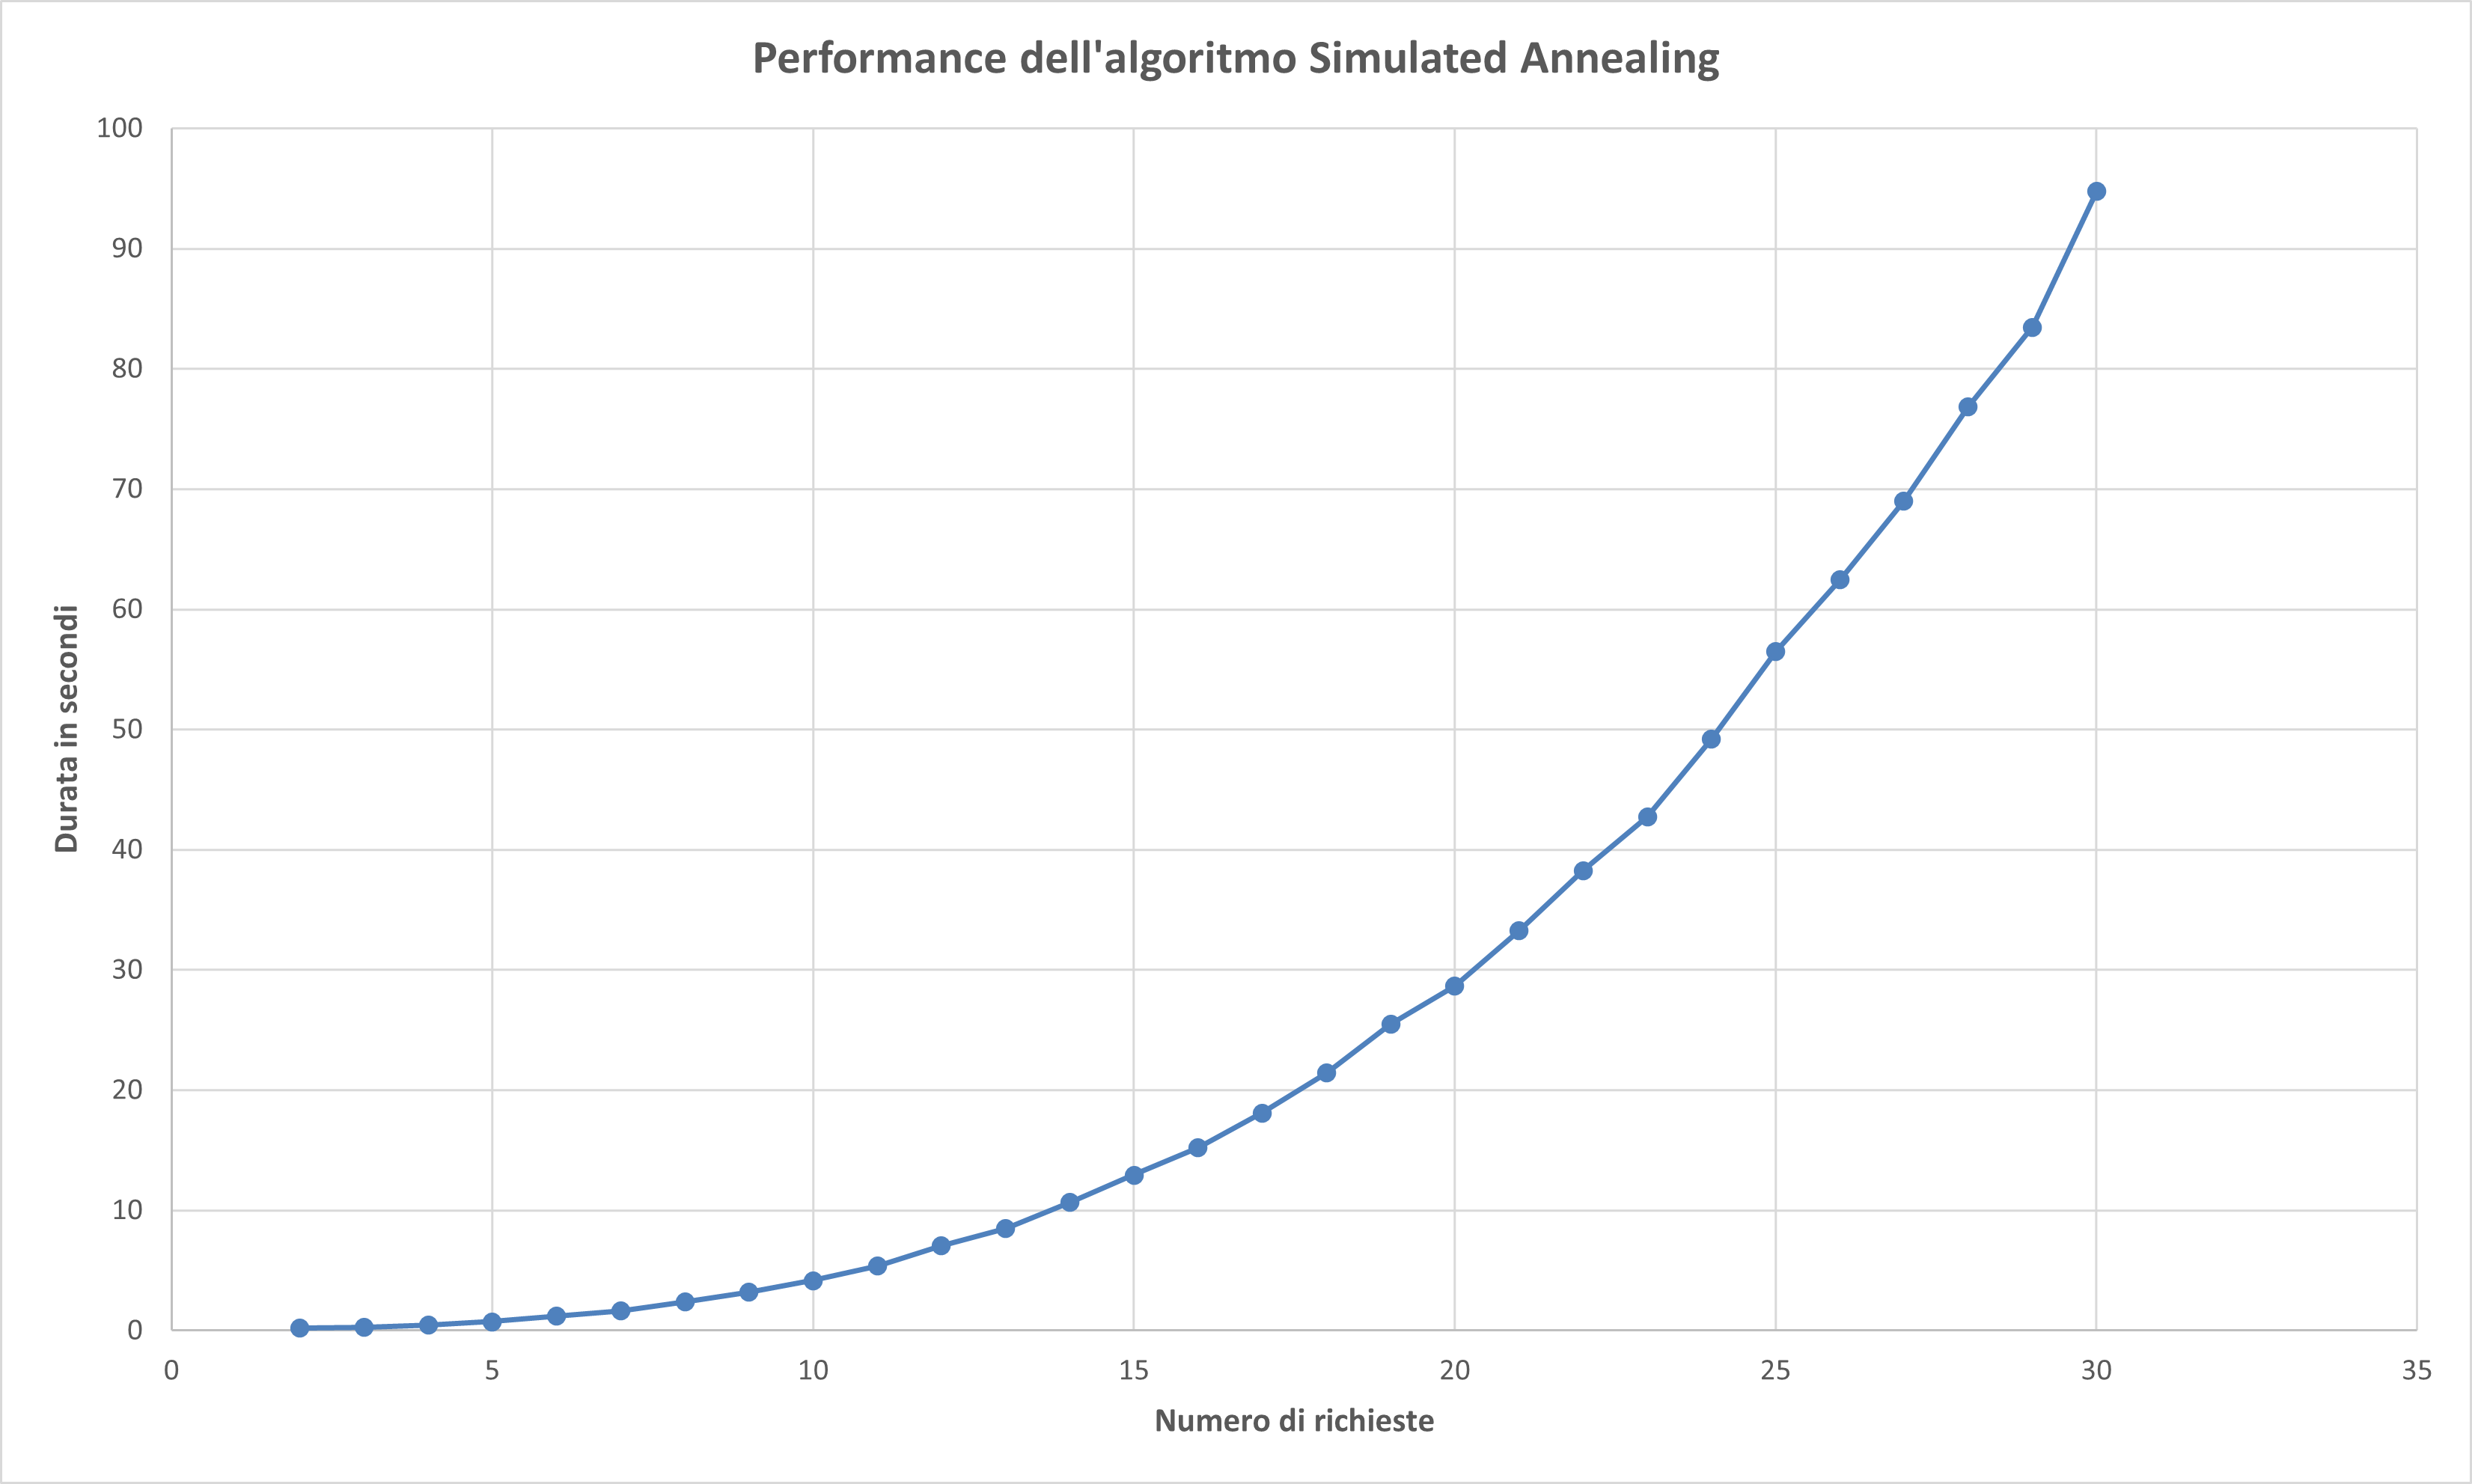
\includegraphics[width=\textwidth]
	{../charts/11 Performance dell'algoritmo Simulated Annealing}
	\end{figure}
\end{frame}

%%%
%%%   TABU SEARCH
%%%
\subsection{Tabu search}
\begin{frame}[allowframebreaks, fragile]{\subsecname}

	\textbf{Descrizione dell'algoritmo} \\
	Ad ogni iterazione si seleziona la miglior soluzione dell’intorno, diversa dalla soluzione corrente, anche peggiore, così da poter sfuggire al bacino di attrazione dell’ottimo locale in cui mi trovo (mantenendo comunque in memoria le soluzioni migliori visitate). \\
	Per evitare loop, e ritornare nello stesso bacino di attrazione utilizzo la \emph{Tabu List} di dimensione fissata. \\
	L’algoritmo termina (stop condition) nel caso in cui il massimo numero di iterazioni sia stato raggiunto oppure sia stato raggiunto il massimo numero di passi senza miglioramenti (stalllo). \\
	\textbf{Eccezioni:} il criterio di aspirazione permette di visitare soluzioni tabù con valore di funzione obiettivo migliore di quella dell’ottimo candidato (sono sicuramente soluzioni mai visitate). \\

\framebreak
	\textbf{Note} \\
	Nella lista tabù memorizzo le mosse proibite. Se durante la ricerca scambio due nodi (29 e 39) allora la mossa da memorizzare è [39,29].
Prima di scegliere una nuova soluzione dovrò sempre controllare che i due nodi selezionati per lo scambio non siano già presenti nella Tabu List.

	\textbf{Parametri utilizzati nell'algoritmo}
	\begin{itemize}
		\item
		Soluzione iniziale: la migliore soluzione ottenuta dalle greedy
		\item
		Intorno utilizzato: city swap
		\item
		Dimensione della tabu list: 20
		\item
		Numero massimo di iterazioni: 20
		\item
		Stallo massimo: 15
	\end{itemize}

	\textbf{Codice} \\
	\href{https://github.com/michele-vaccari/TSP-con-pick-up-and-delivery/blob/main/src/tsppd/solver/tabuSearch.py}{https://github.com/michele-vaccari/TSP-con-pick-up-and-delivery/blob/main/src/tsppd/solver/tabuSearch.py}

\framebreak

	\textbf{Schema dell'algoritmo}
\begin{minted}[fontsize=\tiny, escapeinside=;;, tabsize=2]{c}
// Step 1 (init)
k = 1
Build an initial solution ;$S_{1}$;
;$S_{best} = S_{1}$;

// Step 2 (explore neighborhood)
;$At\,iter\,k$;
	;$select\,S_{c} \neq S_{k} \in Neighborhood(S_{k})$; // possibily the best in ;$N(S_{k})$;
	if ;$f(S_{c}) < f(S_{best})$; then	
		;$S_{best} := S_{c} , S_{k+1} := S_{c}$;
		goto Step 3 // aspiration criteria
	if ;$the\,move\,that\,transforms\,S_{k} \rightarrow S_{c} \in tabu-list$; then
		goto Step 2 	// skip ;$S_{c}$;
	else // the move ;$S_k \leftarrow S_{c}\,is\,not\,forbidden$;
	      ;$S_{k+1} := S_{c}$; // update current solution
		;$insert\,the\,inverted\,move\,(S_{c} \rightarrow S_{k})\,in\,the\,tabu\,list$;
		;$remove\,the\,last\,tabu\,move\,from\,the\,tabu-list$; // FIFO policy
goto Step 3

// Step 3 (stop or loop)
k = k + 1
if (stopping condition = true) then STOP
	return(;$S_{best}$;)
else
	goto Step 2
\end{minted}

\framebreak
	\textbf{Performance nel tempo}
      	\begin{figure}[h]
	\centering
	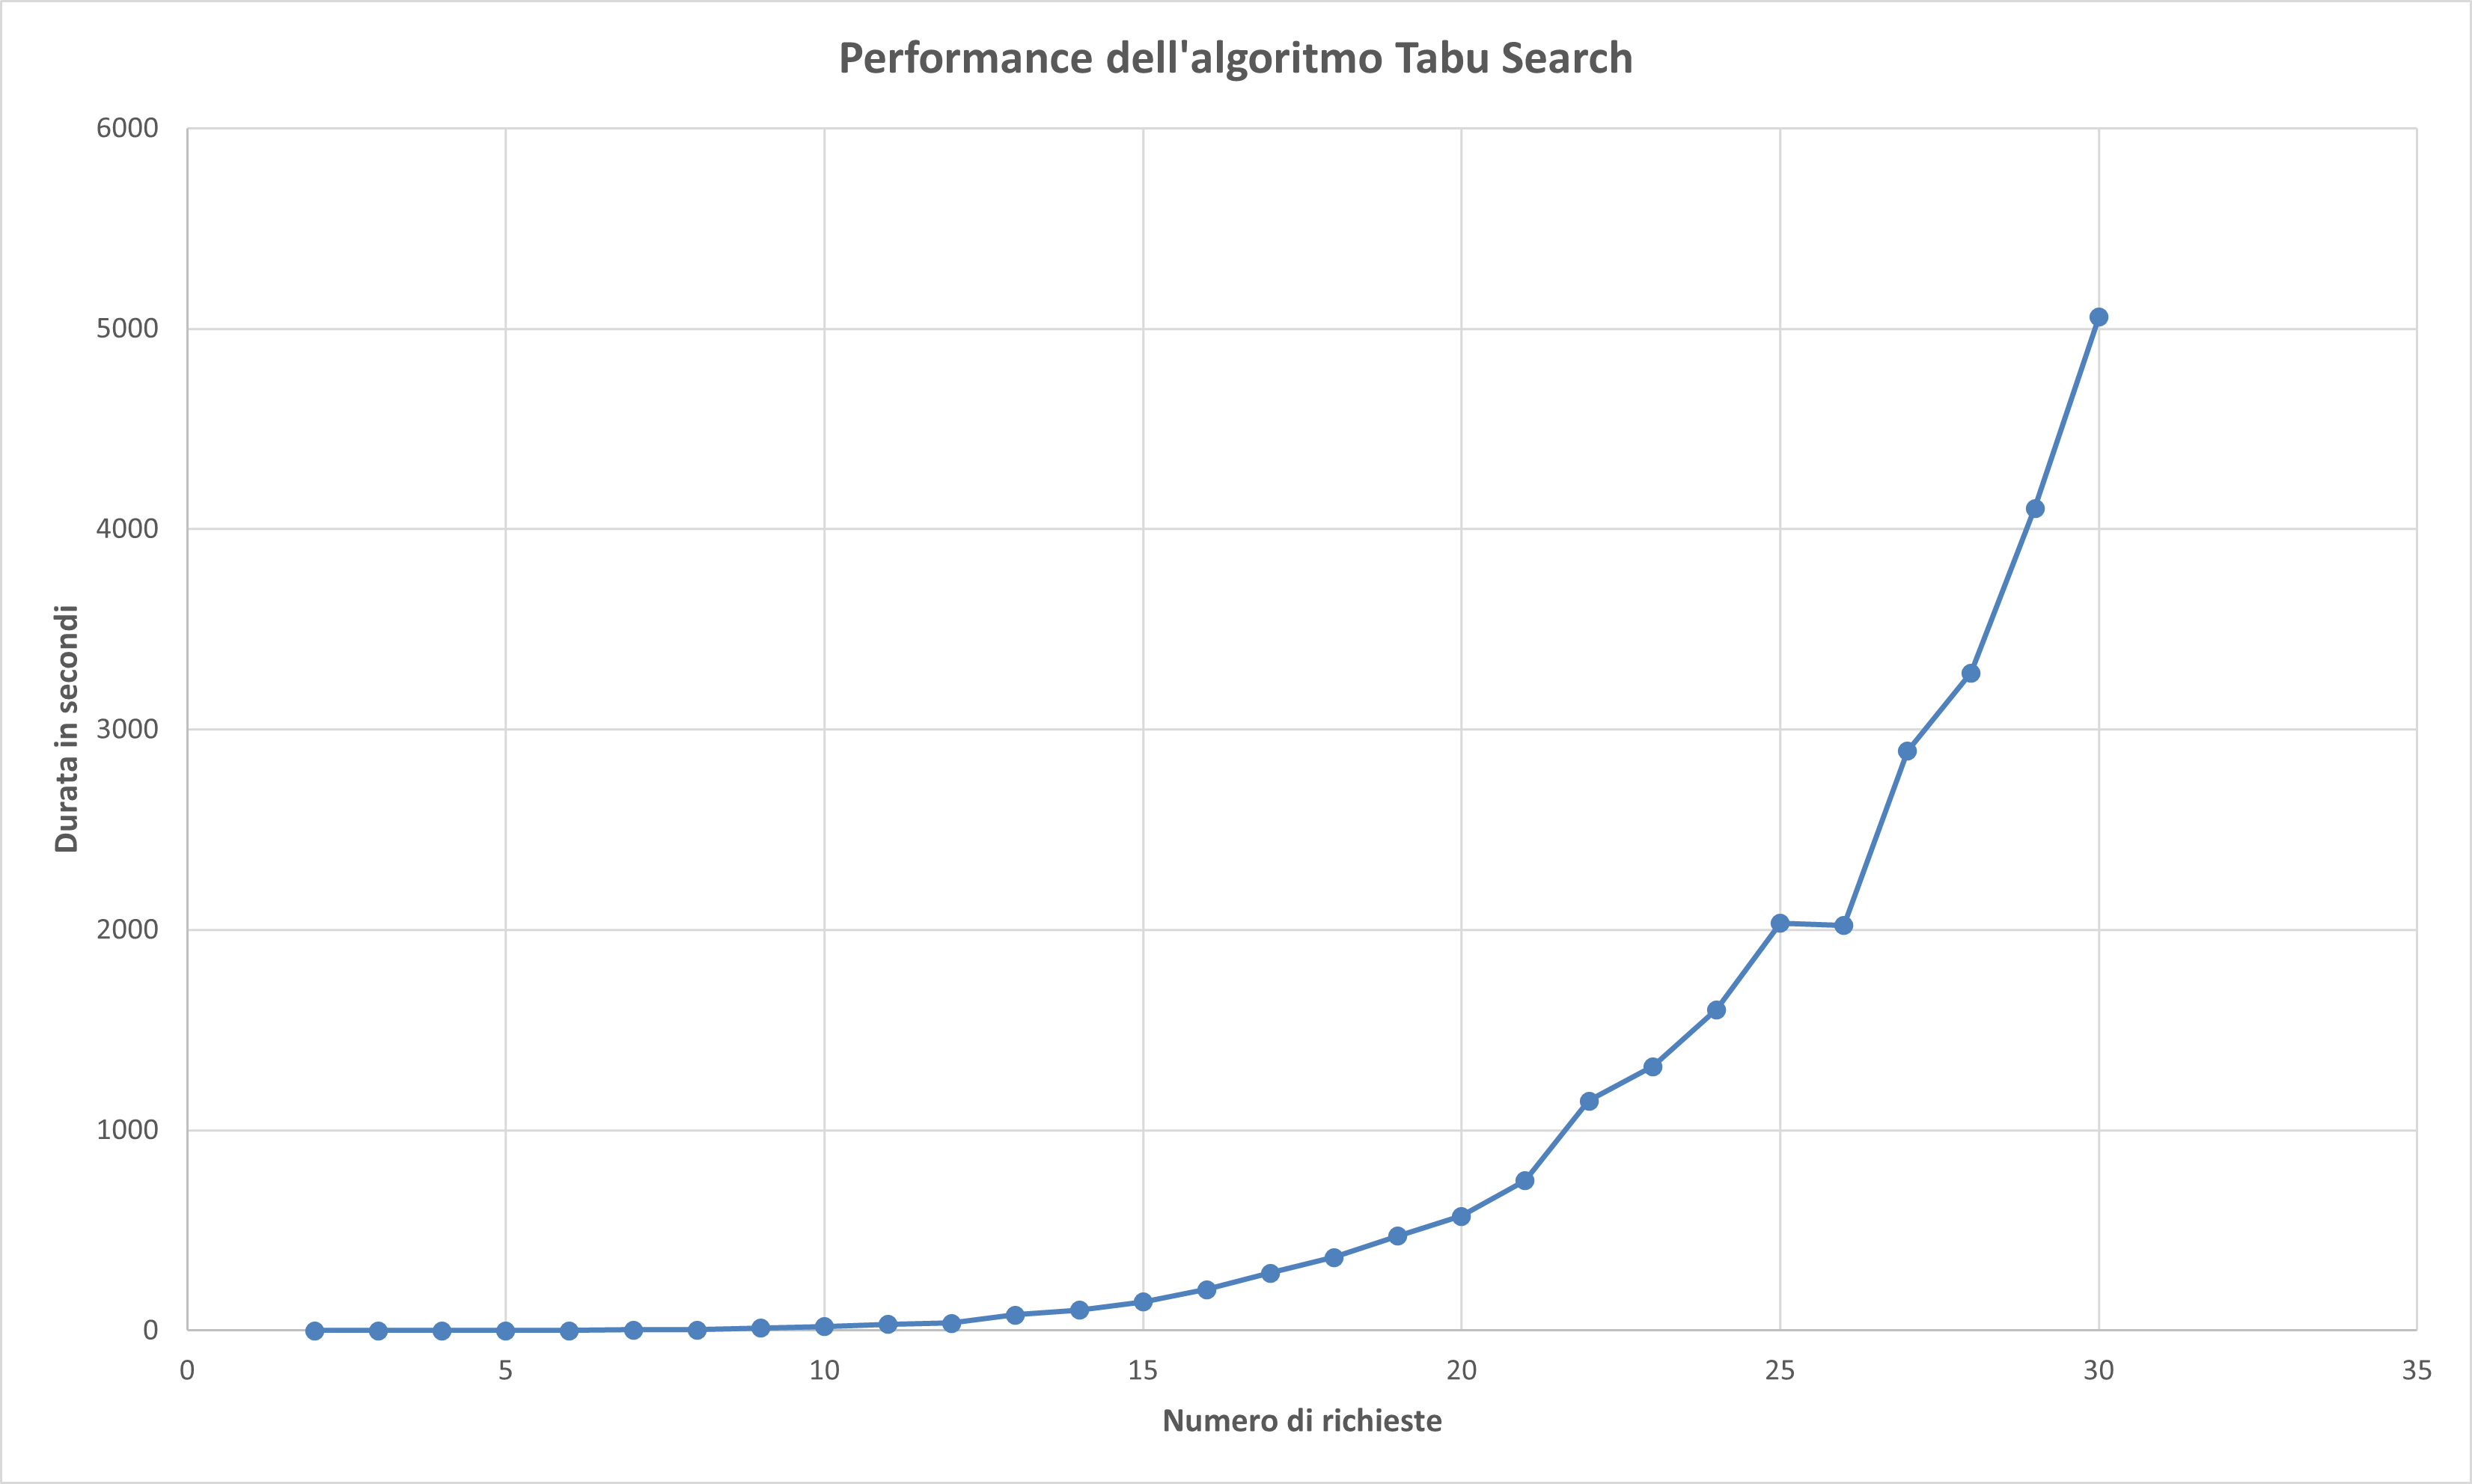
\includegraphics[width=\textwidth]
	{../charts/12 Performance dell'algoritmo Tabu Search}
	\end{figure}
\end{frame}

%%%
%%%   VERY LARGE SIZE NEIGHBORHOOD
%%%
\subsection{Very large size neighborhood}
\begin{frame}[allowframebreaks, fragile]{\subsecname}

	\begin{itemize}
		\item
		Per sfuggire agli ottimi locali con strategie che restano nell’ambito della filosofia Local Search è possibile utilizzare intorni di grandi dimensioni

		\item
		Maggiore è l’ampiezza dell’intorno e migliore la qualità dell’ottimo locale determinato dalla Local Search

		\item
		Esistono diverse strategie da adottare per l’esplorazione di intorni di grandi dimensioni, tipicamente si tratta di strategie non esatte

		\item
		Se la dimensione dell’intorno è vasta, non è possibile operare una esplorazione esaustiva esplicita

		\item
		Una possibilità è individuare un sottoinsieme dell’intorno in modo stocastico campionando casualmente le soluzioni nell’intorno secondo una legge probabilistica
	\end{itemize}

\framebreak

	\begin{itemize}
		\item
		Le strategie di LNS appartengono alla famiglia delle VLNS e sono caratterizzate dal fatto che le soluzioni dell’intorno sono ottenute applicando una mossa di \emph{destroy} e una di \emph{repair}

		\item
		\emph{Destroy} distrugge una parte della soluzione corrente, scelta secondo una procedura non deterministica in modo che la parte modificata vari ad ogni iterazione

		\item
		La procedura di \emph{Repair} deve assegnare valore alle variabili “cancellate” in modo da ripristinare l’ammissibilità (e possibilmente nel modo migliore rispetto alla funzione obiettivo).

		\item
		L’intorno è implicitamente definito dall’insieme di tutte le soluzioni ottenibili applicando le procedure destroy \& repair

		\item
		Il tasso di distruzione (\% delle variabili rimesso in discussione) caratterizza l’intorno che generalmente è esponenziale rispetto alle dimensioni dell’istanza
	\end{itemize}

\framebreak

	\begin{columns}[T,onlytextwidth]
		\column{0.5\textwidth}
\textbf{Template}
\begin{minted}[fontsize=\scriptsize, escapeinside=;;, tabsize=2]{c}
Procedure ;$Large\,Neighborhood\,Search$;
;$x^{0}$; = GenerateInitialSolution
k = 0
;$x^{*}$; = ;$x^{k}$;
repeat
	;$x^{’}$; = rep (dest(;$x^{k}$;))
	if accept(;$x^{’}$;, ;$x^{k}$;) then ;$x^{k}$; = ;$x^{’}$;, k = k + 1
	if c(;$x^{k}$;) < c(;$x^{*}$;) then ;$x^{*}$; = ;$x^{k}$;
until StopCondition
return (;$x^{*}$;)
end
\end{minted}
		\column{0.5\textwidth}
		\textbf{Descrizione dell’algoritmo} \\
		{\scriptsize
		La procedura mantiene 3 variabili:
		\begin{itemize}
			\item
			$x^{*}$ la migliore soluzione trovata (ottimo candidato)
			\item
			$x^{’}$ la nuova soluzione tentativo
			\item
			$x^{k}$ la soluzione corrente all’iterazione k
		\end{itemize}
		$dest(.)$ e $rep(.)$ sono gli operatori di destroy e repair. \\
		La funzione $accept$ può essere implementata in vari modi, il più semplice secondo il criterio di improvement rispetto alla soluzione corrente (accetto solo se miglioro). \\
		LNS non esplora l’intorno ma lo campiona, come nel \emph{Simulated Annealing}.

		}
	
	  \end{columns}

\framebreak

	\textbf{Parametri utilizzati nell'algoritmo}
	\begin{itemize}
		\item
		Soluzione iniziale: la migliore soluzione ottenuta dalle greedy
		\item
		Operatore destroy: rimuovo dalla soluzione un numero di nodi pari al tasso di distruzione (non rimuovo il primo e l’ultimo nodo, è il nodo deposito)
		\item
		Tasso di distruzione: 0.3
		\item
		Operatore repair: procedura ``hand made``. Prima ricolloco i nodi di pickup e, ogni volta che reinserisco un nodo nella soluzione cerco di reinserirlo nel modo ottimale (in modo che il costo della soluzione sia minimo). Poi ricolloco i nodi di delivery e, ogni volta che reinserisco un nodo nella soluzione cerco di reinserirlo nel modo ottimale (in modo che il costo della soluzione sia minimo).
		\item
		Criterio di stop: ho raggiunto 2 miglioramenti oppure ho raggiunto 100 peggioramenti
	\end{itemize}

	\textbf{Codice} \\
	\href{https://github.com/michele-vaccari/TSP-con-pick-up-and-delivery/blob/main/src/tsppd/solver/largeNeighborhoodSearch.py}{https://github.com/michele-vaccari/TSP-con-pick-up-and-delivery/blob/main/src/tsppd/solver/largeNeighborhoodSearch.py}

\framebreak

	\textbf{Performance nel tempo}
      	\begin{figure}[h]
	\centering
	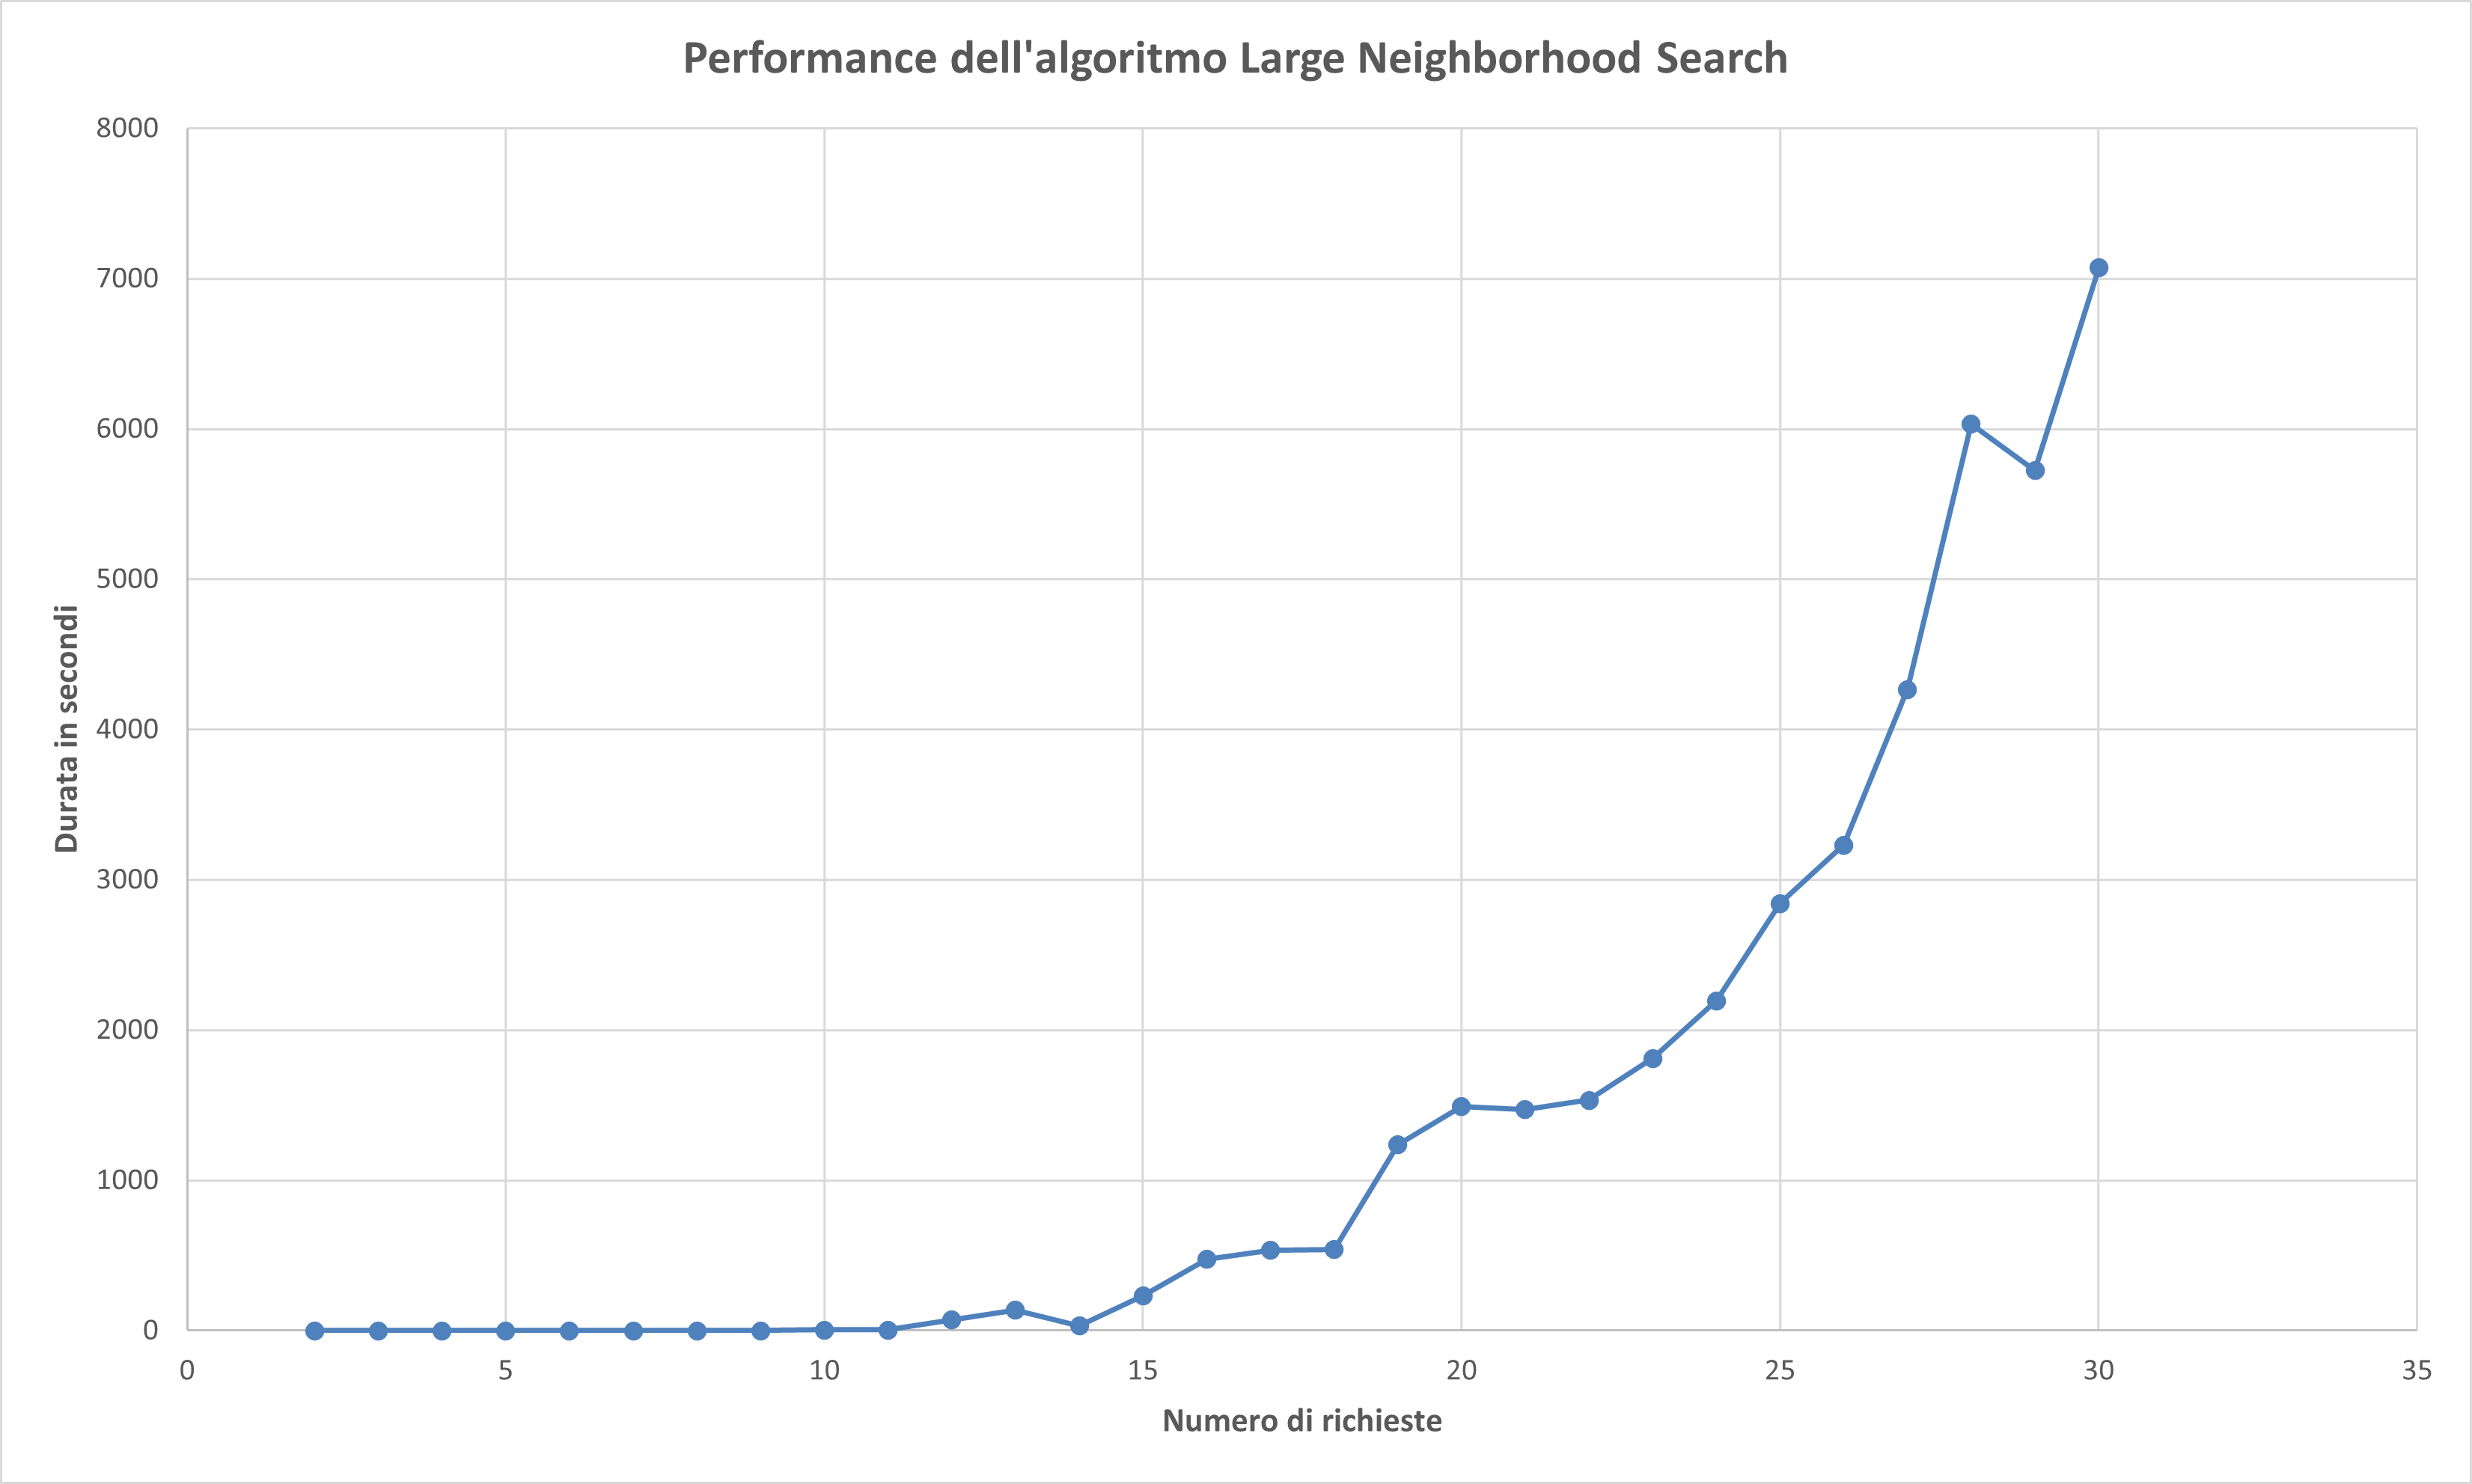
\includegraphics[width=\textwidth]
	{../charts/13 Performance dell'algoritmo Large Neighborhood Search}
	\end{figure}

\end{frame}

%%%
%%%   MULTI START LOCAL SEARCH
%%%
\subsection{Multi Start Local Search}
\begin{frame}[allowframebreaks]{\subsecname}

	\begin{itemize}
	
		\item
		Per sfuggire agli ottimi locali con strategie che restano nell’ambito della filosofia Local Search è possibile \emph{agire sul punto di arrivo uscendo dall’ottimo locale corrente} attraverso una mossa di \emph{diversificazione} che sposti il punto corrente, da cui riprendere la ricerca, nel bacino di attrazione di un altro ottimo locale

		\item
		Studi sperimentali hanno comprovato che per problemi di ottimizzazione combinatoria numerosi ottimi locali sono di bassa qualità

		\item
		Quindi è ragionevole cercare una strategia per continuare la ricerca anche dopo avere determinate un ottimo locale

		\item
		Ad esempio iterando il procedimento a partire da un altro punto iniziale

		\item
		\emph{Occorre una strategia per il restart} che sfrutti il fatto che statisticamente le buone soluzioni sono clusterizzate

		\item
		Quindi piuttosto che ripartire da un punto casuale è meglio perturbare l’ottimo locale corrente
		
	\end{itemize}

\framebreak

	\textbf{Definizione dell'algoritmo} \\
	Itero più volte una ricerca locale, ogni volta partendo da un punto iniziale diverso

	\textbf{Codice} \\
	\href{https://github.com/michele-vaccari/TSP-con-pick-up-and-delivery/blob/main/src/tsppd/solver/multiStartLocalSearch.py}{https://github.com/michele-vaccari/TSP-con-pick-up-and-delivery/blob/main/src/tsppd/solver/multiStartLocalSearch.py}

	\textbf{Parametri utilizzati nell'algoritmo}
	\begin{itemize}
		\item
		Iterazioni massime: 10
		\item
		Strategia per partire da un punto diverso: Greedy random (random restart / blind search)
		\item
		Local Search utilizzata: Large Neighborhood Search
		\item
		Criterio di stop: numero massimo di iterazioni raggiunto
	\end{itemize}

\framebreak

	\textbf{Rischi}
	\begin{itemize}
		\item
		Se due soluzioni iniziali appartengono allo stesso bacino di attrazione, la ricerca converge allo stesso ottimo locale
		\item
		La generazione totalmente random del punto iniziale non permette un controllo a priori
	\end{itemize}

\framebreak

	\textbf{Performance nel tempo}
      	\begin{figure}[h]
	\centering
	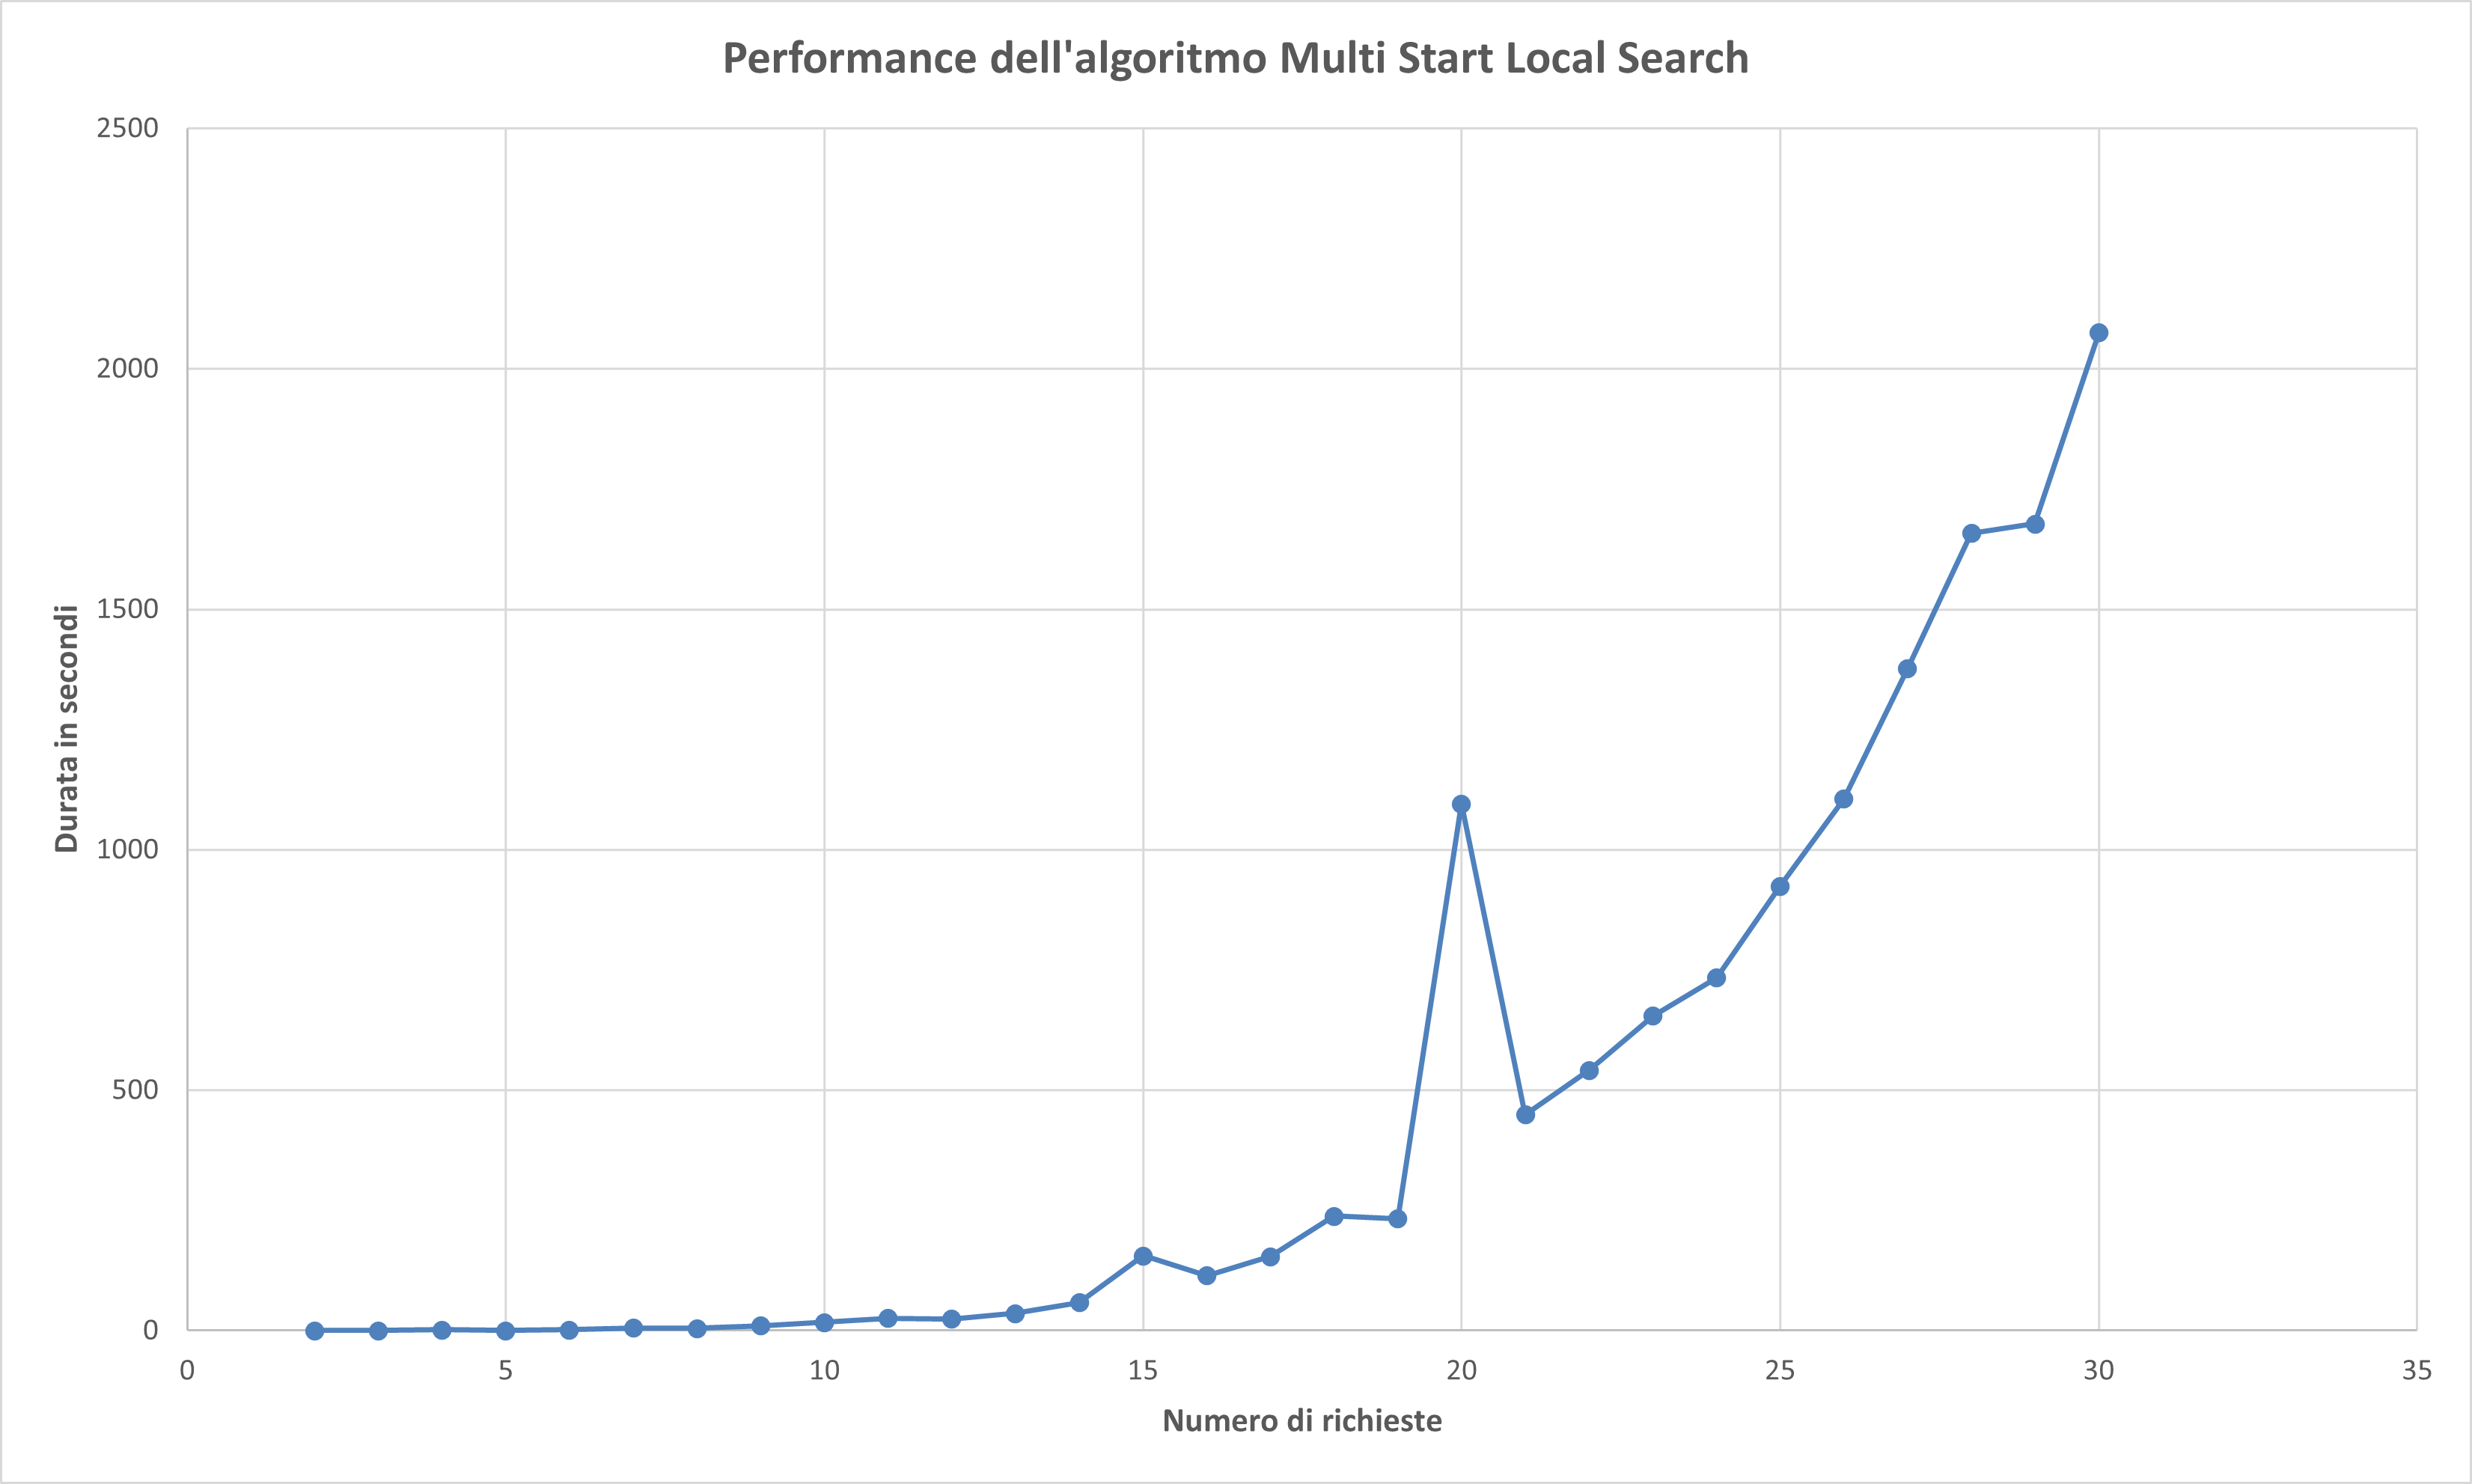
\includegraphics[width=\textwidth]
	{../charts/14 Performance dell'algoritmo Multi Start Local Search}
	\end{figure}

\end{frame}

%%%
%%%   GREEDY RANDOMIZED ADAPTIVE SEARCH PROCEDURE
%%%
\subsection{Greedy Randomized Adaptive Search Procedure}
\begin{frame}[allowframebreaks]{\subsecname}

	\begin{itemize}
	
		\item
		Per sfuggire agli ottimi locali con strategie che restano nell’ambito della filosofia Local Search è possibile agire \emph{moltiplicando i punti di partenza} e riapplicare una nuova LS a partire da ciascuno di essi

		\item
		È naturale pensare a un algoritmo greedy per la costruzione della soluzione ammissibile di partenza di una ricerca locale

		\item
		Con le sole greedy e ricerca locale possiamo già creare delle meta-euristiche che forniscono risultati migliori dei singoli algoritmi

		\item
		Le \emph{Meta-euristiche} sono metodi risolutivi che orchestrano una interazione tra procedure locali di miglioramento e strategie di livello superiore che permettono di sfuggire agli ottimi locali, e operare una esplorazione il più possibile robusta (indipendente dal punto di partenza) della regione ammissibile

		\item
		La Multi Start Local Search applica ripetutamente una ricerca locale LS a partire da punti iniziali diversi ottenuti in modo casuale. La generazione random dei punti iniziali ha i seguenti svantaggi:
		\begin{itemize}
			\item
			nessuna garanzia sulla \emph{qualità} della \emph{soluzione iniziale}, il che richiede molto sforzo computazionale per la fase iniziale della ricerca per migliorare una soluzione mediocre
			\item
			spesso sono punti che appartengono al bacino di attrazione di ottimi locali (\emph{soluzione finale di ogni LS}) non molto buoni
			\item
			potenzialmente si converge più volte allo stesso ottimo locale (quando più punti iniziali appartengono allo stesso bacino di attrazione)
		\end{itemize}

		\item
		La Greedy Randomized Adaptive Search Procedure è un’evoluzione della Multi Start Local Search. Intervenendo sulla generazione dei punti iniziali della Multi Start Local Search in modo tale da avere contemporaneamente le seguenti condizioni:
		\begin{itemize}
			\item
			garantire una sufficiente diversità delle soluzioni prodotte all’iterare della procedura, tale che le soluzioni appartengano a bacini di attrazione di ottimi locali diversi, per non convergere più volte allo stesso ottimo locale
			\item
			spesso sono punti che appartengono al bacino di attrazione di ottimi locali (\emph{soluzione finale di ogni LS}) non molto buoni
			\item
			non perdere troppo nella qualità della soluzione iniziale per non investire troppo nella prima fase di ogni LS
		\end{itemize}
		
	\end{itemize}

\framebreak

	\textbf{Definizione dell'algoritmo} \\
	\textbf{\footnotesize Passo 1: Greedy \& Random} \\
	Ad ogni passo della greedy seleziono a caso un elemento tra i migliori $k$ (dimensione della restricted candidate list) \\
	\textbf{\footnotesize Passo 2: Greedy \& Random \& Local Search} \\
	Applico una LS a ciascuna soluzione prodotta dalla greedy randomizzata, e ripetendo $k$ volte la procedura.

	\textbf{Codice} \\
	\href{https://github.com/michele-vaccari/TSP-con-pick-up-and-delivery/blob/main/src/tsppd/solver/greedyRandomizedAdaptiveSearchProcedure.py}{https://github.com/michele-vaccari/TSP-con-pick-up-and-delivery/blob/main/src/tsppd/solver/greedyRandomizedAdaptiveSearchProcedure.py}

\framebreak

	\textbf{Parametri utilizzati nell'algoritmo}
	\begin{itemize}
		\item
		Iterazioni massime: 10
		\item
		Dimensione della restricted candidate list: 20
		\item
		Strategia per partire da un punto diverso: scelgo a caso un elemento dalla restricted candidate list
		\item
		Local Search utilizzata: Large Neighborhood Search
		\item
		Criterio di stop: numero massimo di iterazioni raggiunto
	\end{itemize}

\framebreak

	\textbf{Performance nel tempo}
      	\begin{figure}[h]
	\centering
	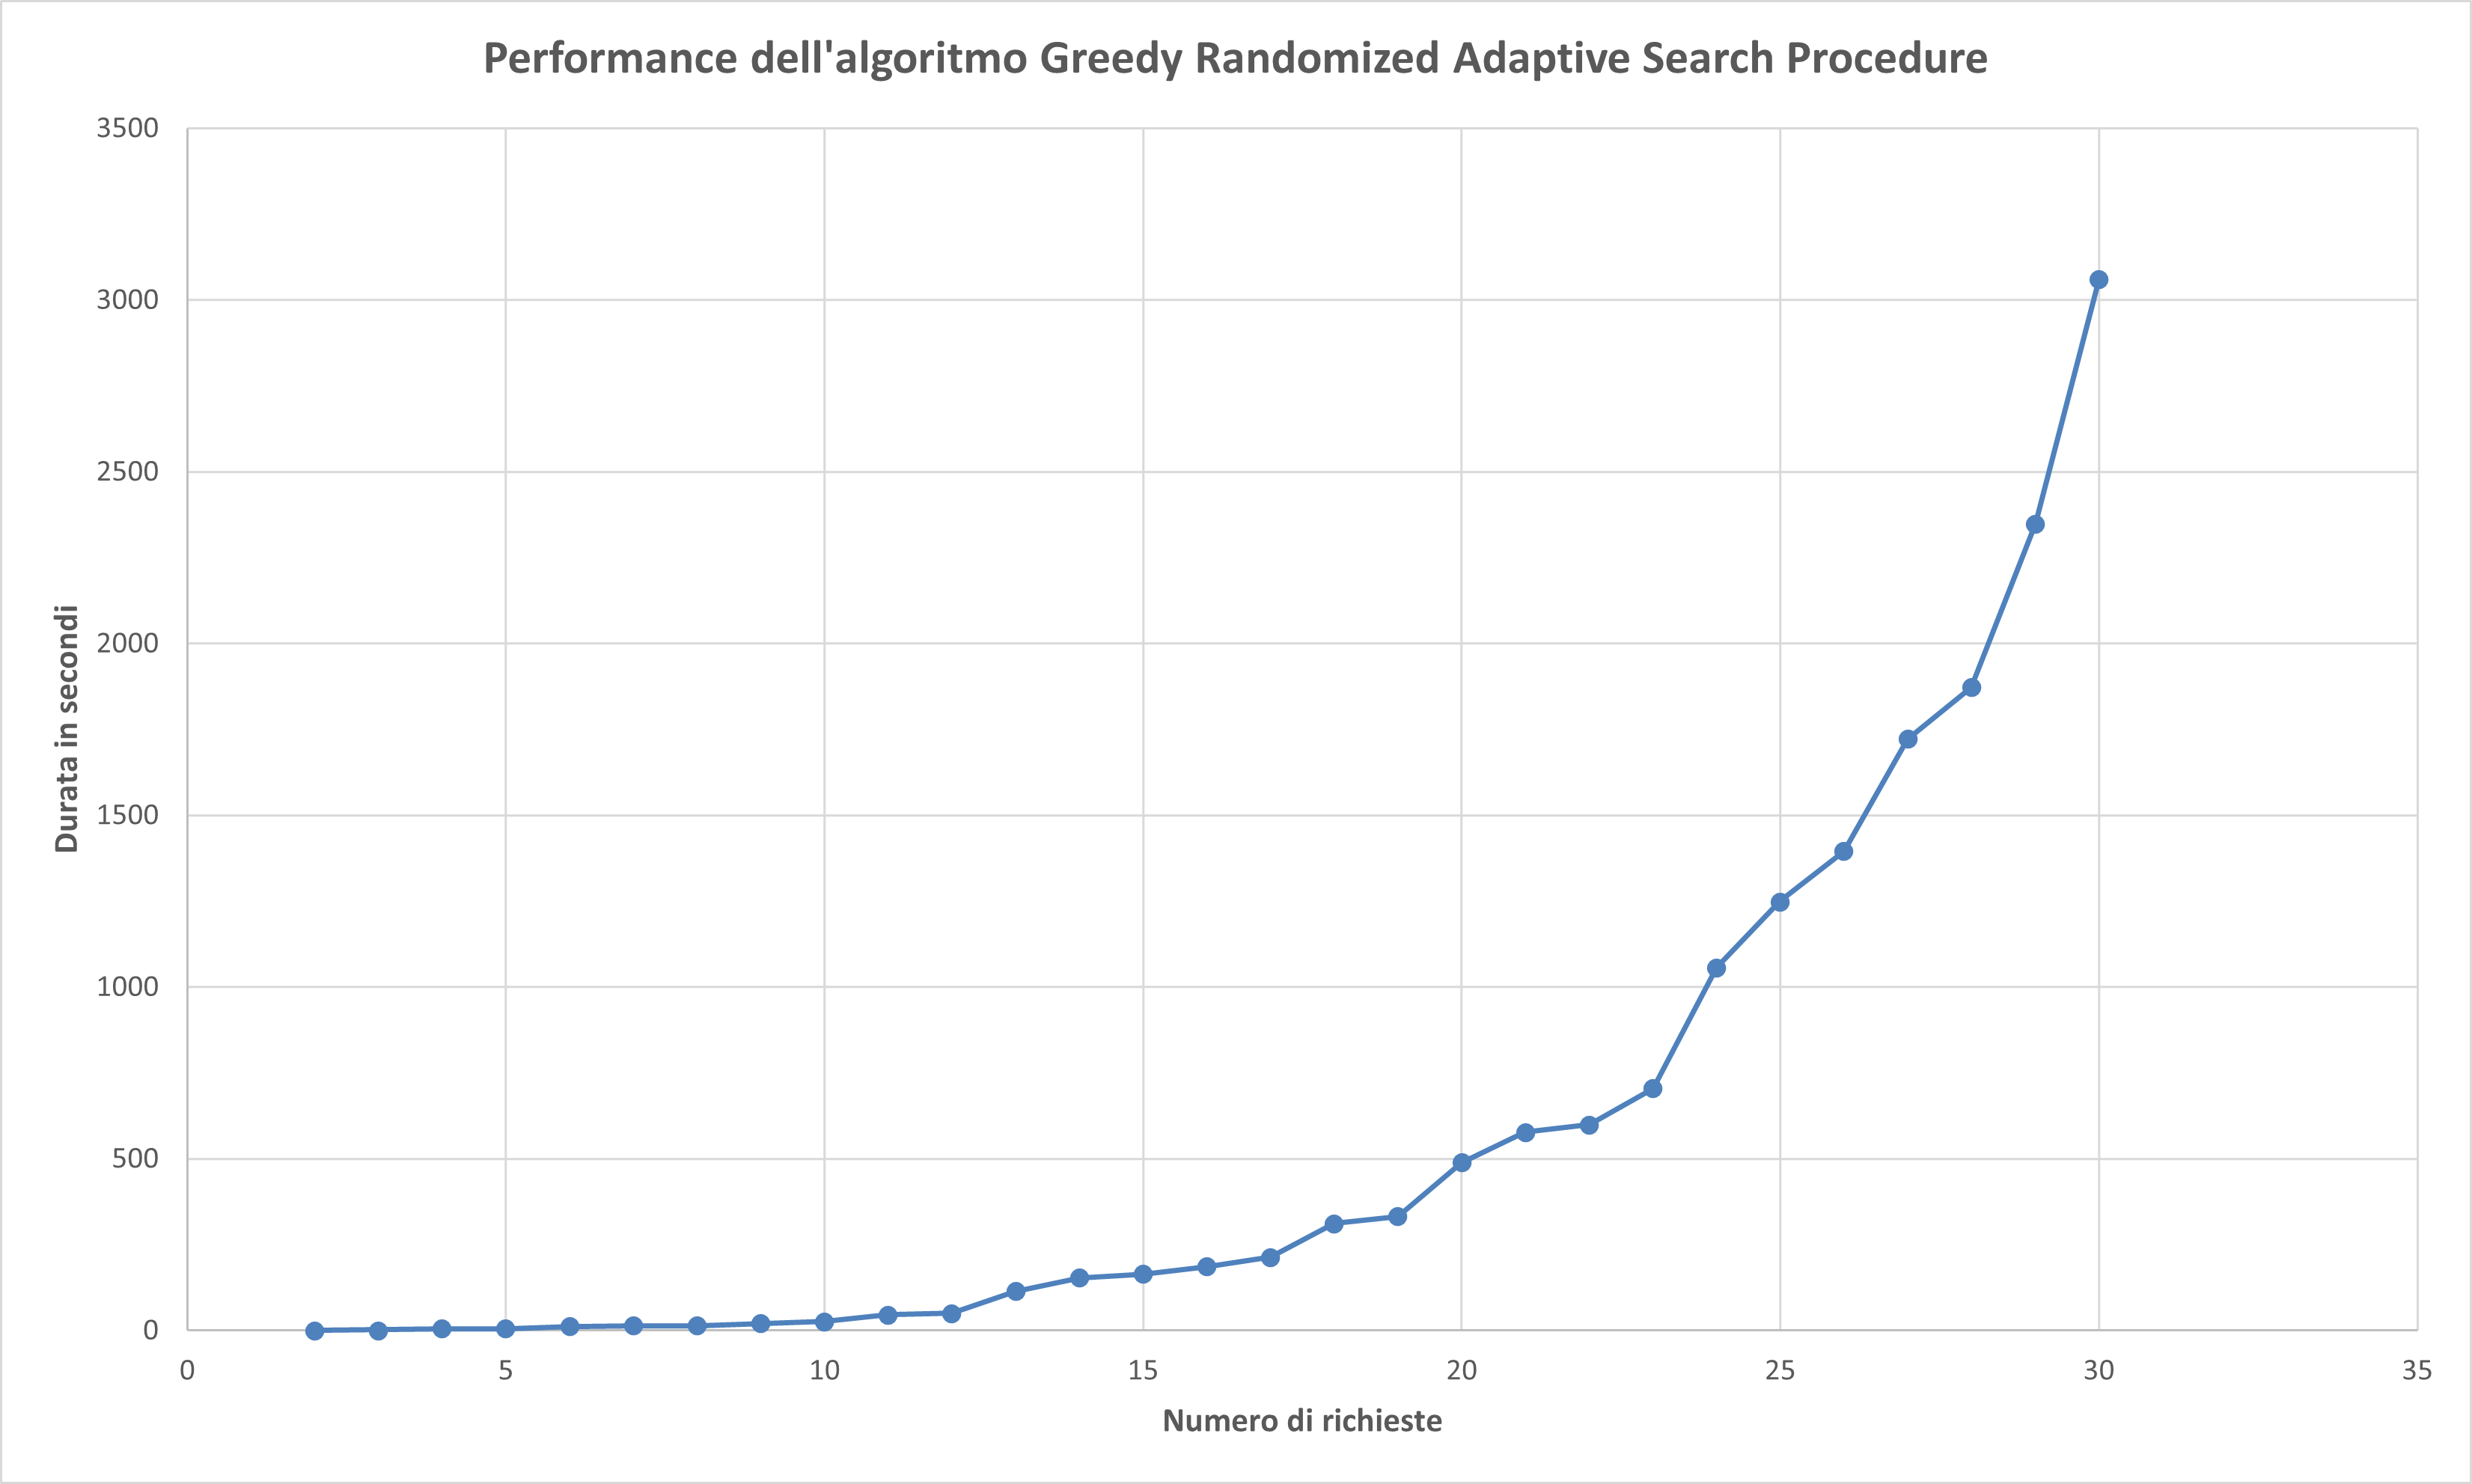
\includegraphics[width=\textwidth]
	{../charts/15 Performance dell'algoritmo Greedy Randomized Adaptive Search Procedure}
	\end{figure}

\framebreak

	Un limite è dato dalla mancanza di memoria della procedura. Ogni restart è indipendente dai precedenti. \\
	Guardando al profilo della funzione obiettivo su $F$, spesso si osserva che gli ottimi locali sono concentrati in una regione limitata (Proximate Optimality Principle). \\

	\textbf{Definizione dell'algoritmo} \\
	\textbf{\footnotesize Passo 3: Greedy \& Local Search \& Path Relinking} \\
	Si raccolgono le soluzioni elite, e si opera una ricerca nello spazio ristretto alle soluzioni simili ad esse, secondo una tecnica, detta \emph{PATH RELINKING}, che esplora le soluzioni che si ottengono operando delle mosse a partire da una soluzione elite di partenza $p$ avvicinandosi a una soluzione elite target $t$

	\textbf{Parth Relinking} \\
	Partendo da una soluzione iniziale ($s_i$), con la ricerca locale si ottiene una soluzione target $s^*$. Opero in successione delle mosse di scambio di componenti per avvicinarmi alla soluzione target. In pratica:
	\begin{itemize}
		\item
		Ad ogni passo, la mossa potenziale consiste nel modificare una componente di $s_i$ sostituendola con una del target $s^*$, per ciascuna delle componenti per cui $s_i$ e $s^*$ differiscono. Si procede selezionando la mossa più conveniente
		\item
		Il valore della funzione lungo il percorso non è monotono, ma spesso lungo il percorso si individuano soluzioni migliori sia di $s_i$ che di $s^*$
	\end{itemize}

	\textbf{Codice} \\
	\href{https://github.com/michele-vaccari/TSP-con-pick-up-and-delivery/blob/main/src/tsppd/solver/greedyRandomizedAdaptiveSearchProcedure.py}{https://github.com/michele-vaccari/TSP-con-pick-up-and-delivery/blob/main/src/tsppd/solver/greedyRandomizedAdaptiveSearchProcedure.py}

\framebreak

	\textbf{Performance nel tempo}
      	\begin{figure}[h]
	\centering
	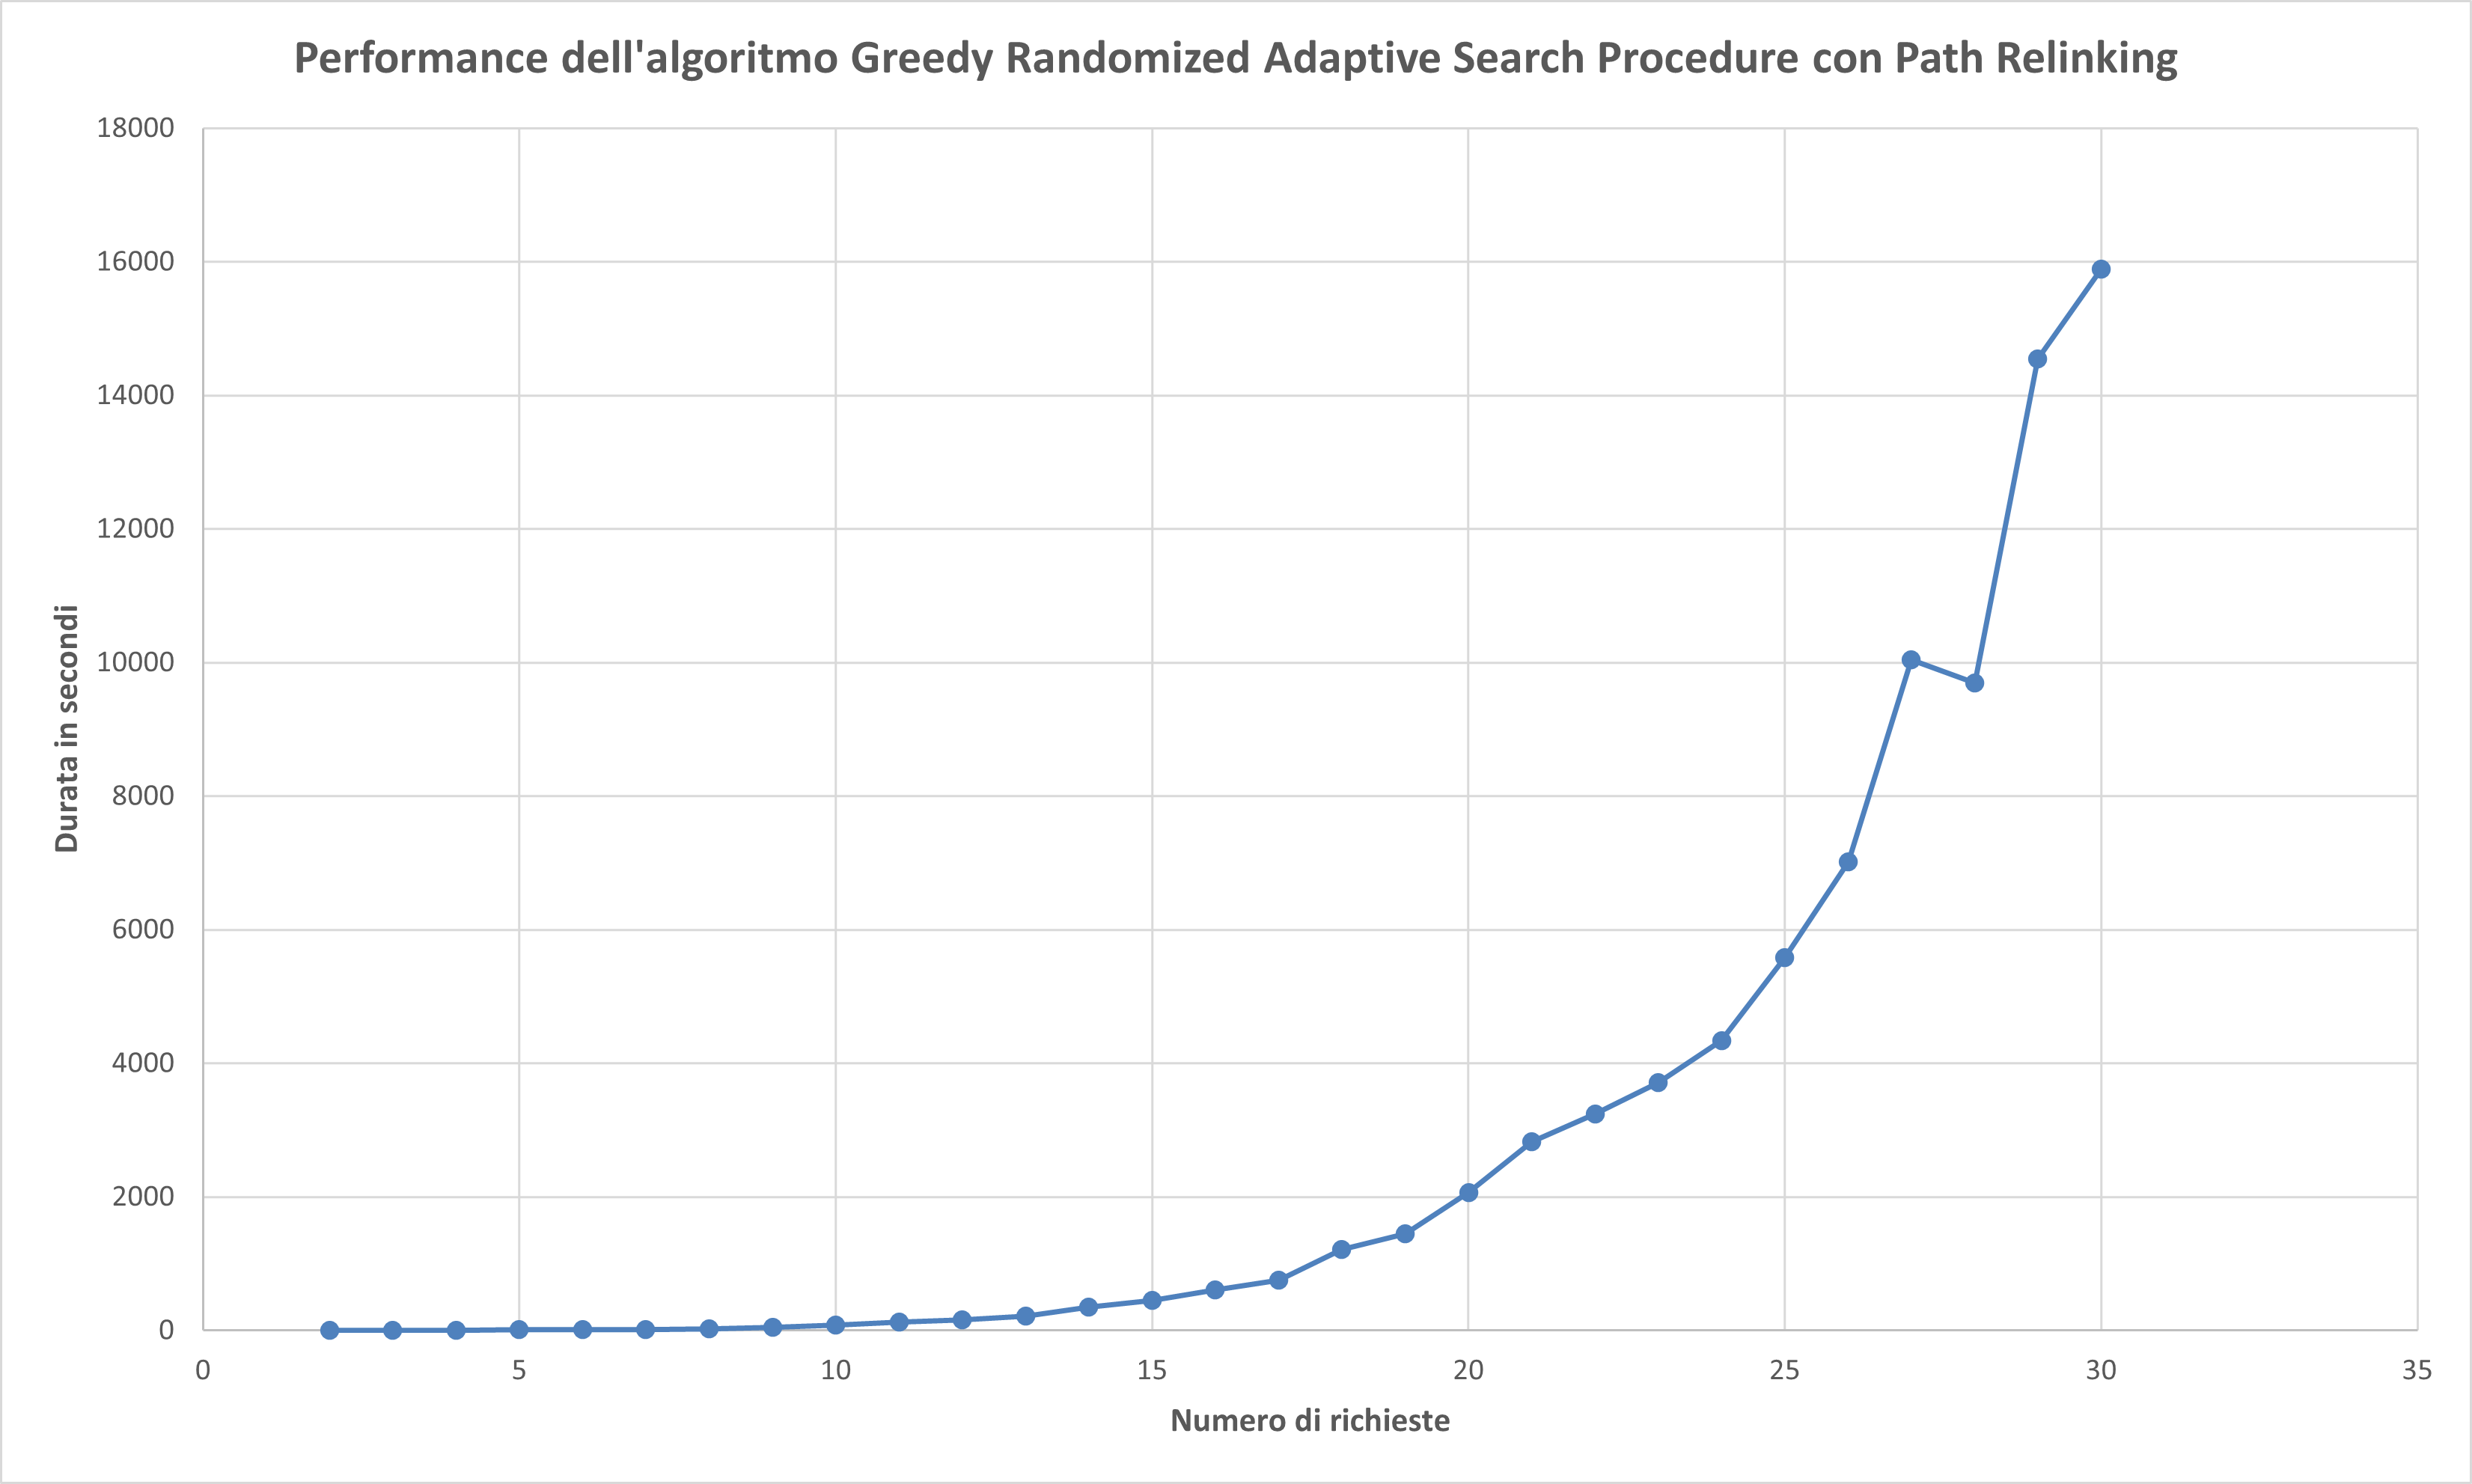
\includegraphics[width=\textwidth]
	{../charts/16 Performance dell'algoritmo Greedy Randomized Adaptive Search Procedure con Path Relinking}
	\end{figure}

\end{frame}

\subsection{Confronto}
\begin{frame}[allowframebreaks]{\subsecname}

	\textbf{Performance nel tempo}
      	\begin{figure}[h]
	\centering
	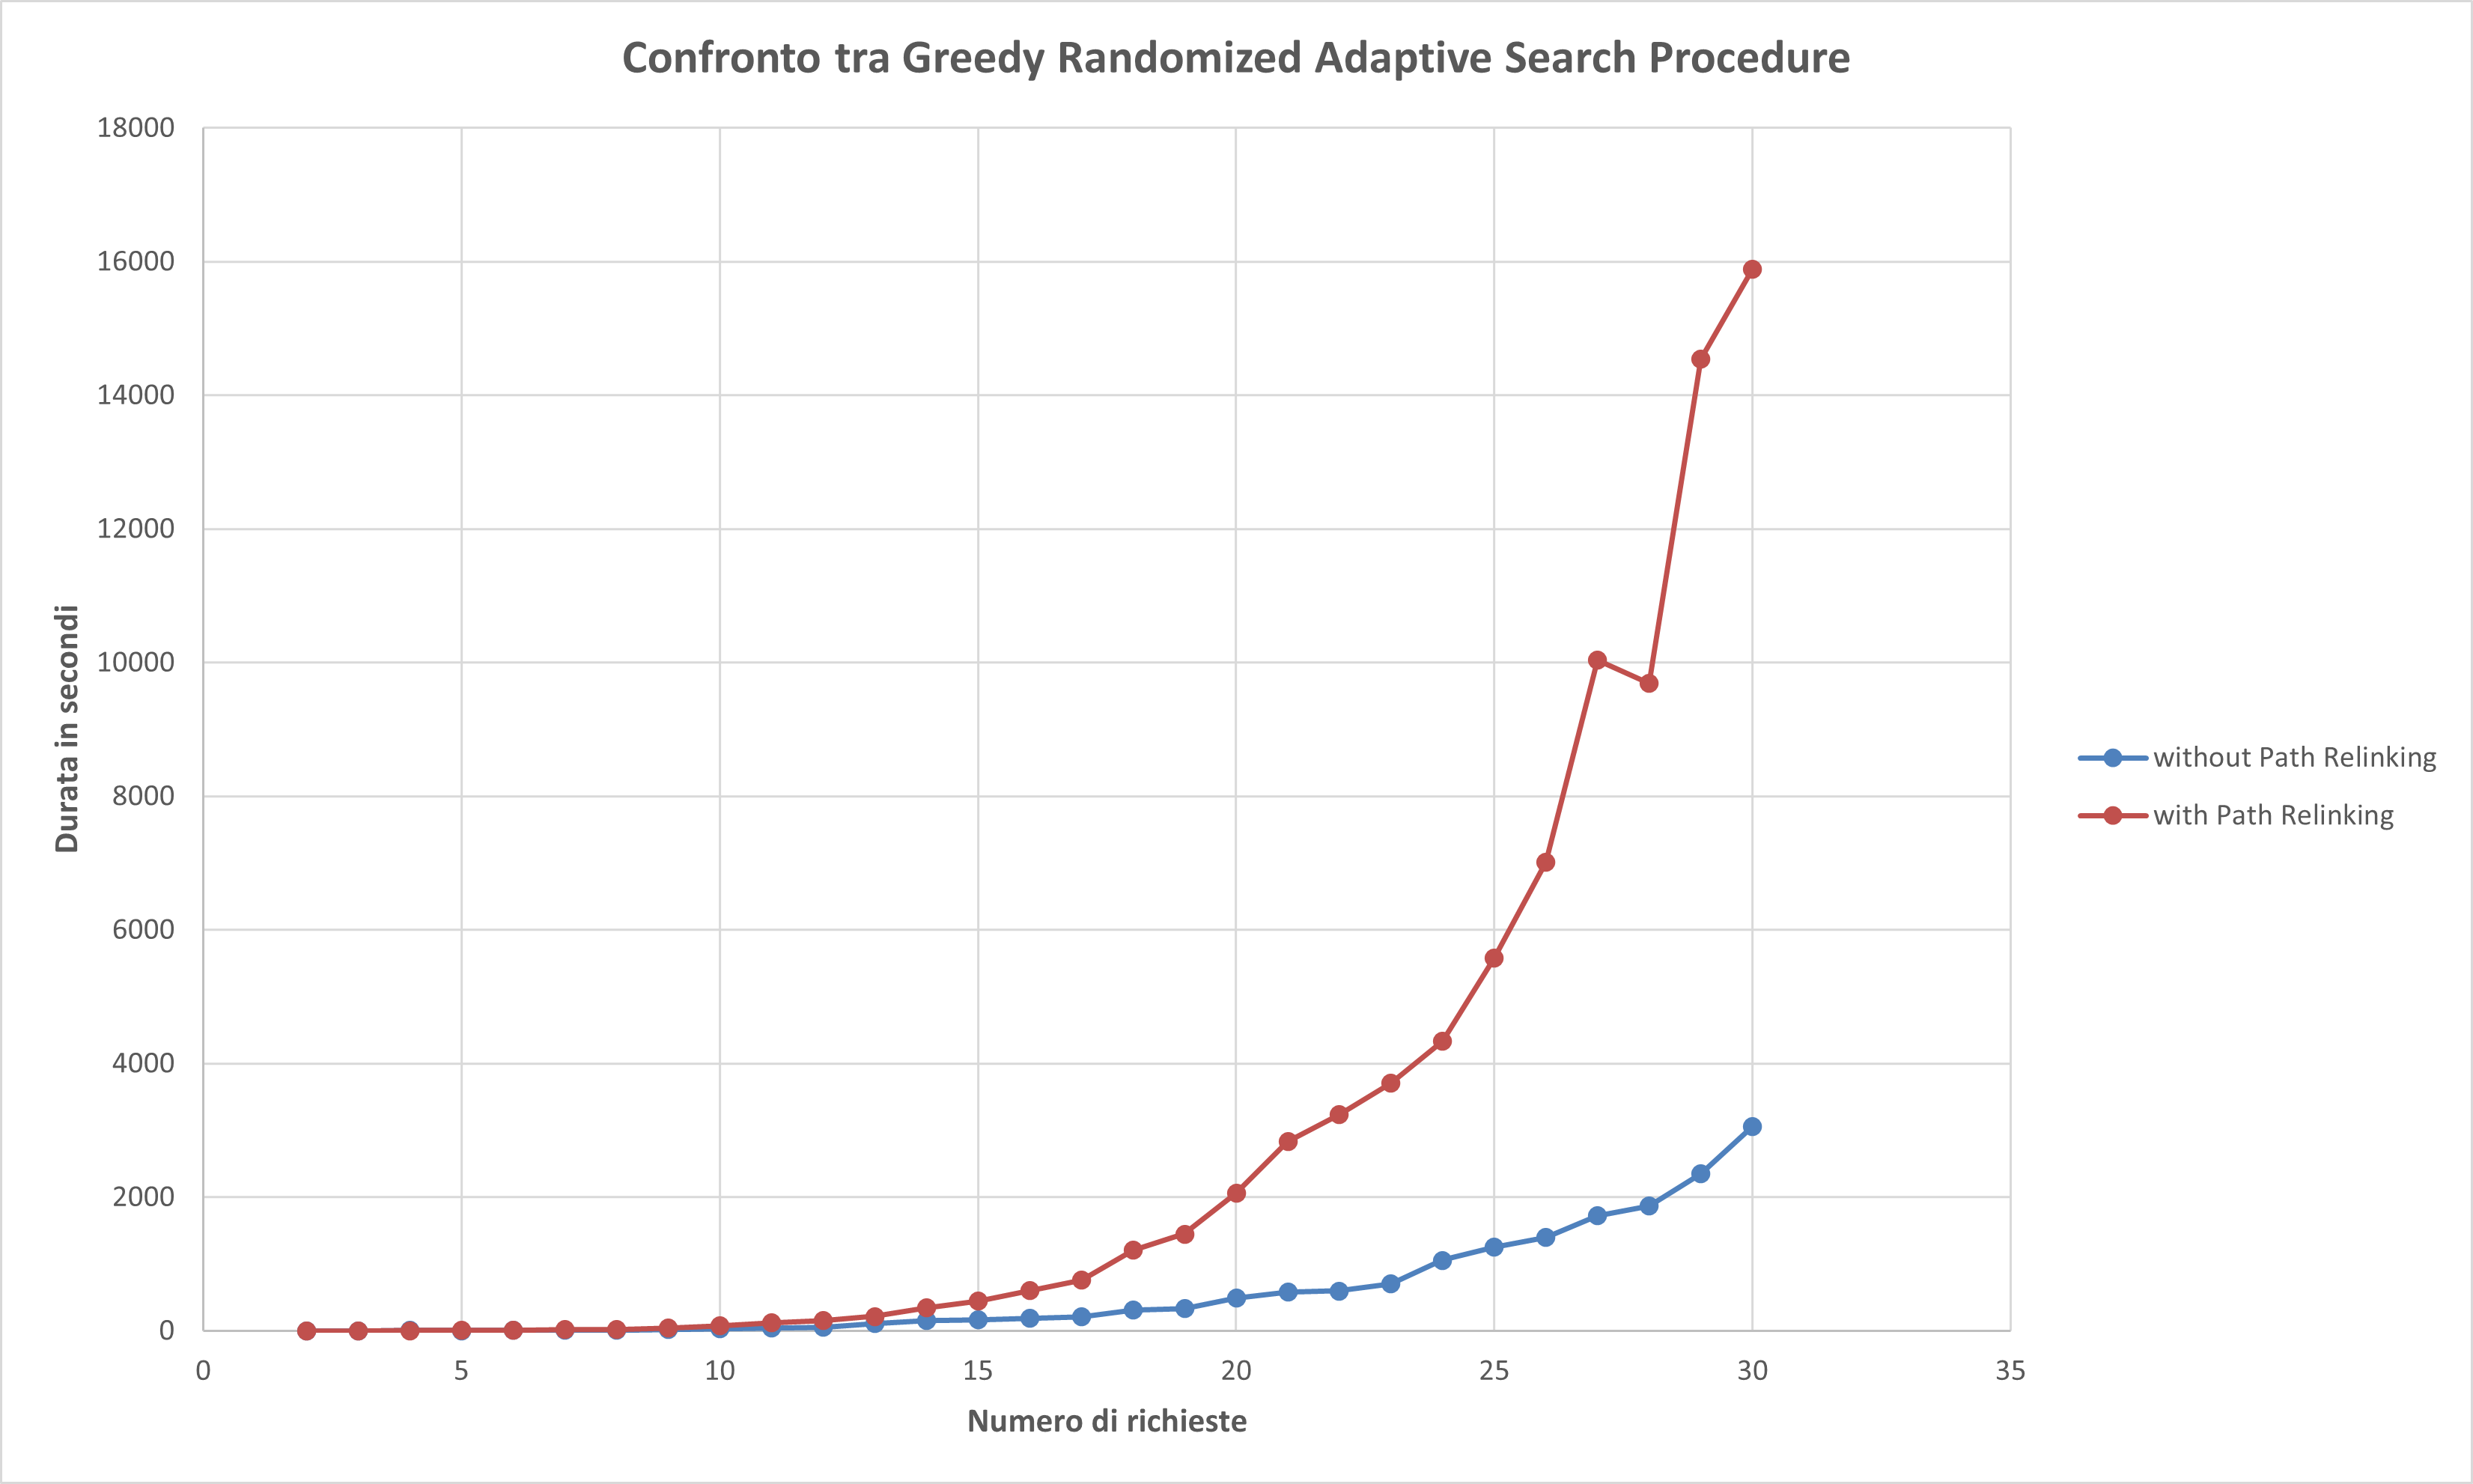
\includegraphics[width=\textwidth]
	{../charts/17a Confronto tra Greedy Randomized Adaptive Search Procedure}
	\end{figure}

\framebreak

	\textbf{Performance costo soluzione}
      	\begin{figure}[h]
	\centering
	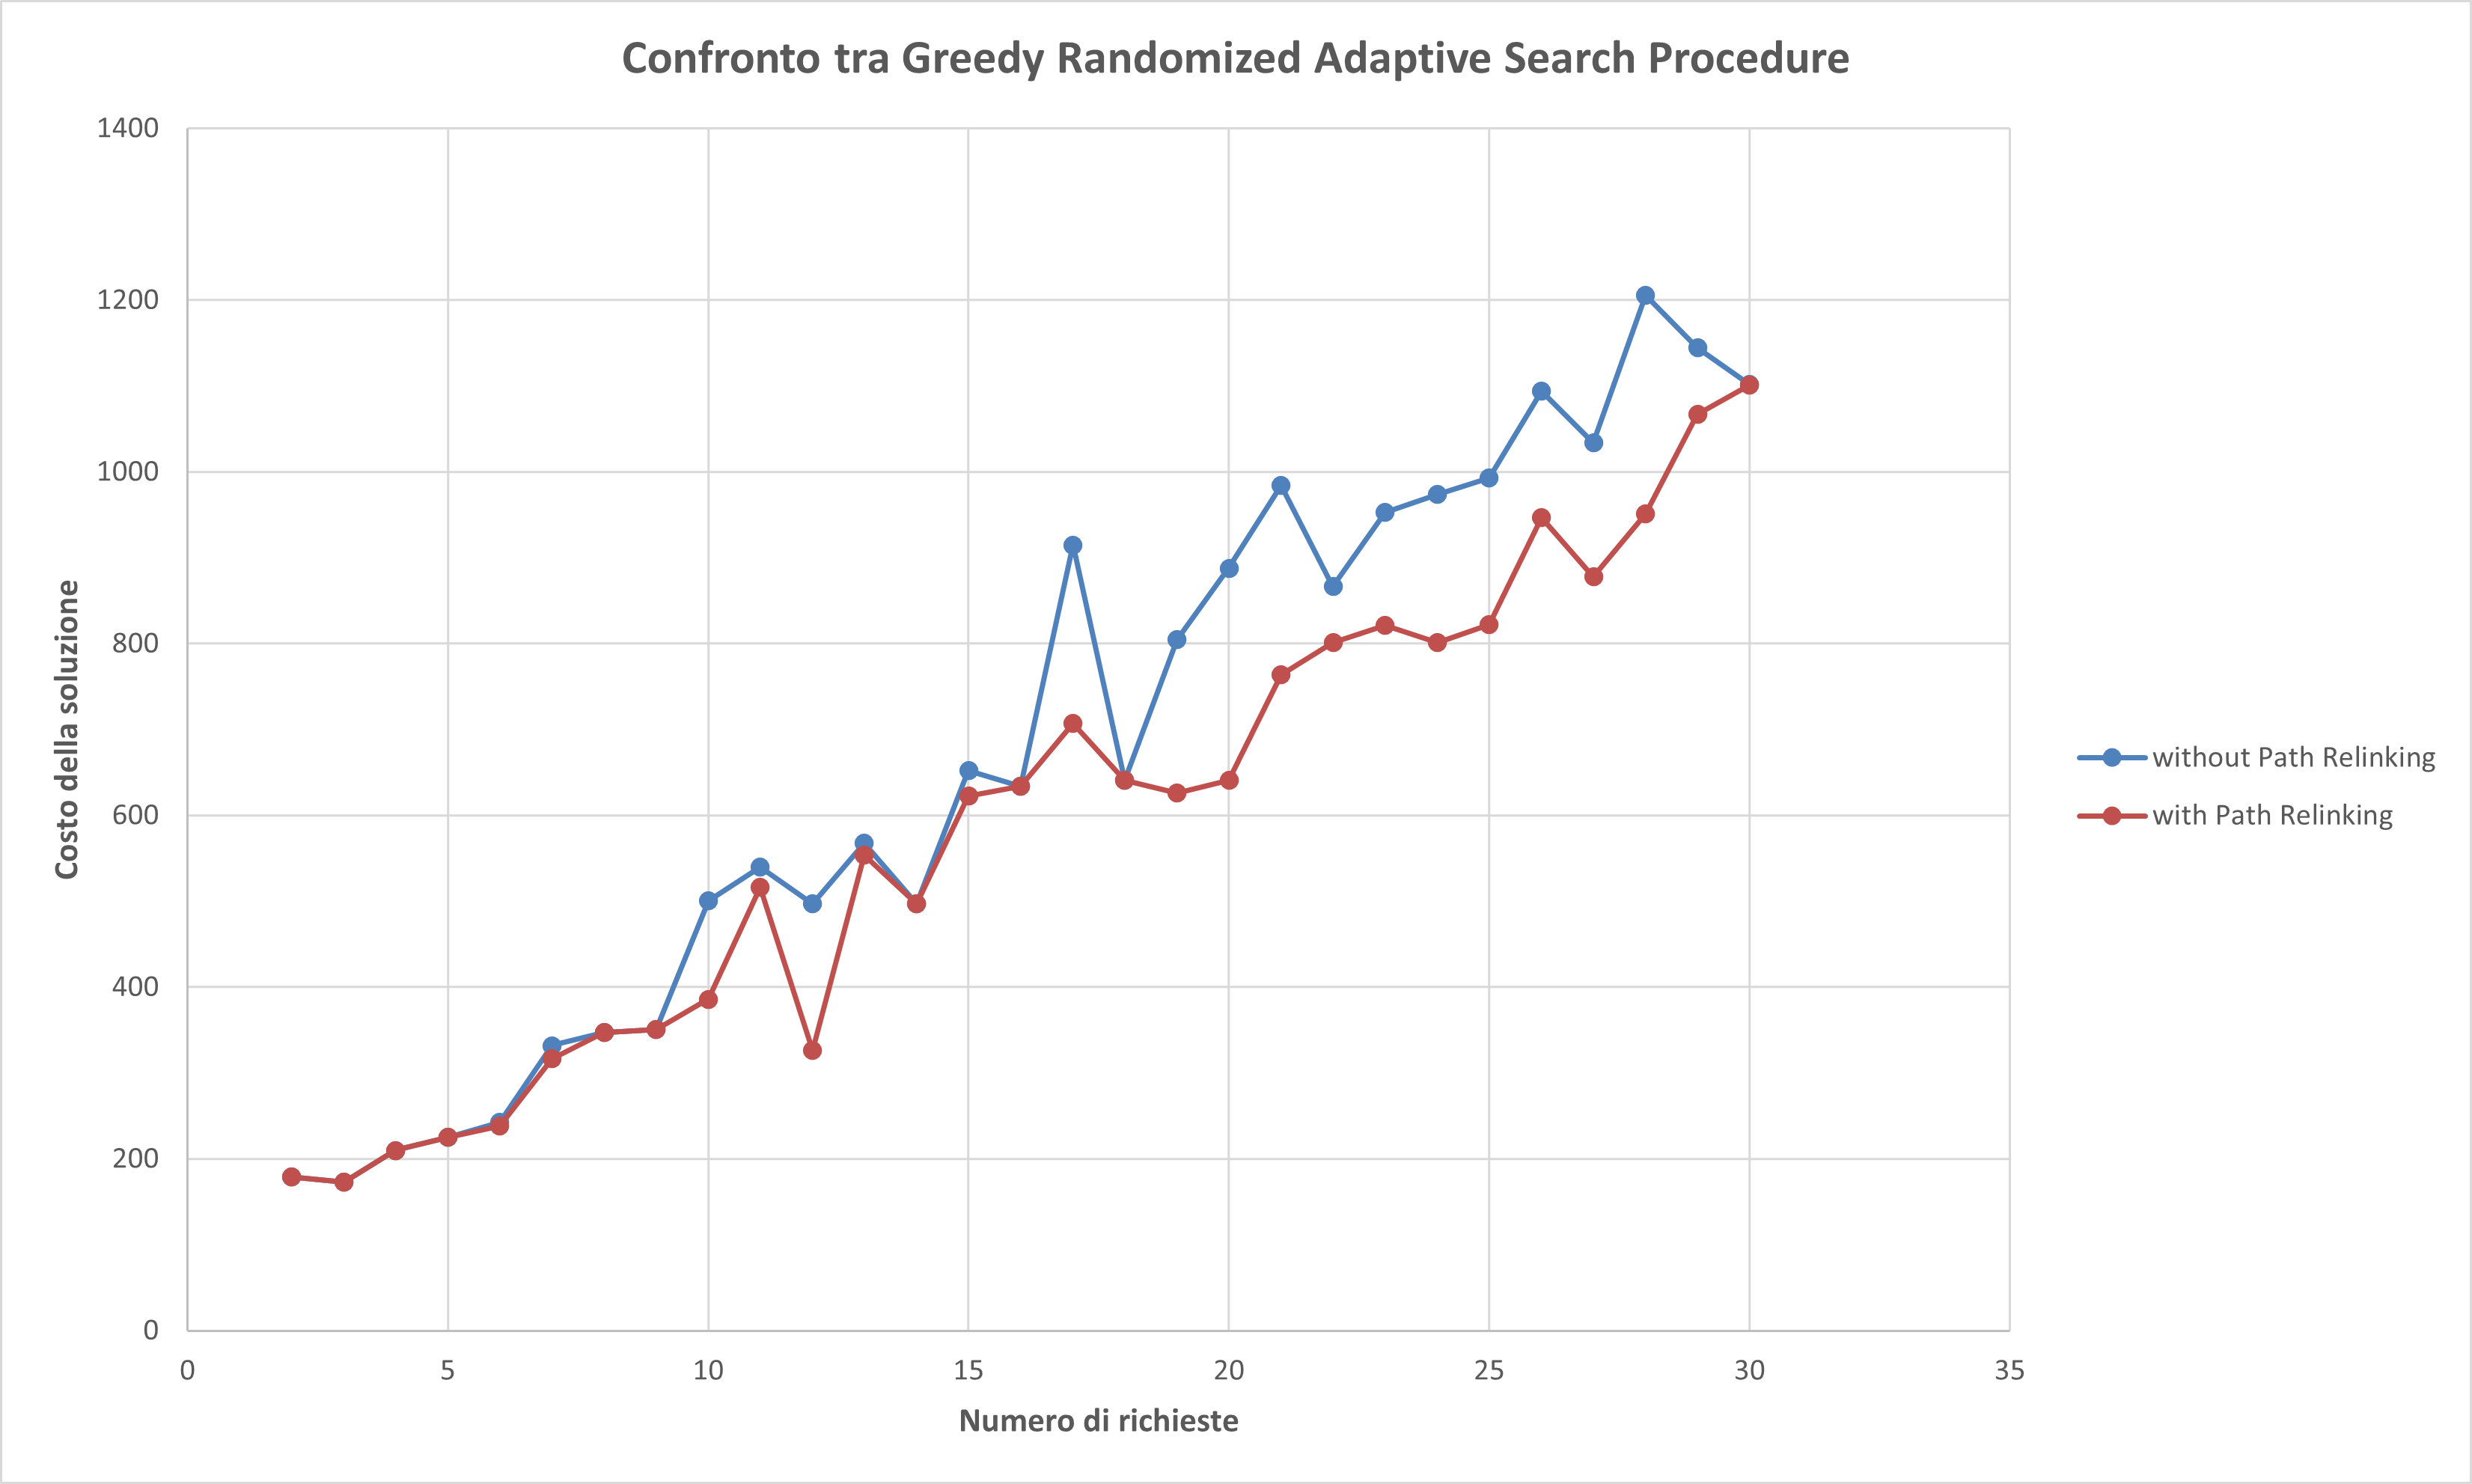
\includegraphics[width=\textwidth]
	{../charts/17b Confronto tra Greedy Randomized Adaptive Search Procedure}
	\end{figure}

\end{frame}

\section{Algoritmi euristici population based}

\subsection{Genetic Algorithm}
\begin{frame}[allowframebreaks]{\subsecname}

	Algoritmi basati sulla teoria dell’evoluzione di Darwin
      	\begin{figure}[h]
	\centering
	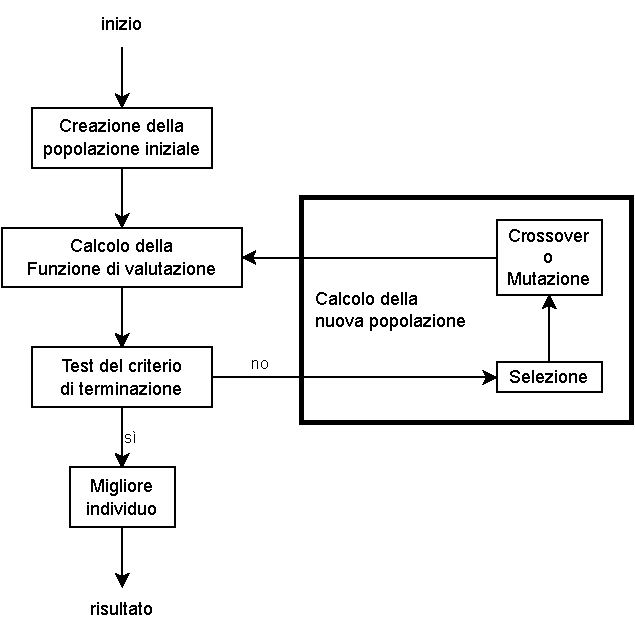
\includegraphics[height=0.65\textheight]
	{../images/block-diagram-genetic-algorithm}
	\caption{Diagramma a blocchi del Genetic Algorithm}
	\end{figure}

\framebreak

	\textbf{Parametri utilizzati nell'algoritmo}
	\begin{itemize}
		\item
		Numero elementi della popolazione iniziale: $\#\;nodi^2$ se $\leq 200$, altrimenti $200$
		\item
		Numero di iterazioni massime: $2 \times \#\;popolazione\;iniziale$ se $\leq 200$, altrimenti $200$
		\item
		Popolazione: generata utilizzando la \emph{Greedy Random}
		\item
		Codifica: lista in ordine di visita dei nodi
		\item
		Metodo di scelta dei genitori: \emph{Roulette Wheel}
		\item
		Crossover: custom (vedi slide \ref{crossover})
		\item
		Elitismo: il migliore individuo passa alla generazione successiva sovrascrivendo il peggiore
		\item
		Tasso di mutazione: 0.3
		\item
		Condizione di stop: numero iterazioni massime raggiunto
	\end{itemize}

	\textbf{Codice} \\
	\href{https://github.com/michele-vaccari/TSP-con-pick-up-and-delivery/blob/main/src/tsppd/solver/geneticAlgorithm.py}{https://github.com/michele-vaccari/TSP-con-pick-up-and-delivery/blob/main/src/tsppd/solver/geneticAlgorithm.py}

\framebreak \label{crossover}
	
	\textbf{Crossover} \\
 	Un individuo è un tour. \\
	Il normale cross over a 1 punto non funziona.

      	\begin{figure}[h]
	\centering
	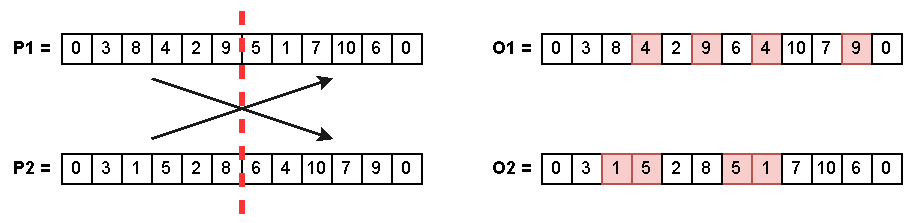
\includegraphics[width=\textwidth]
	{../images/crossover-1a}
	\end{figure}

	I nodi 4, 9, sono visitati 2 volte in O1. \\
	I nodi 1, 5, sono visitati 2 volte in O2.

\framebreak

      	\begin{figure}[h]
	\centering
	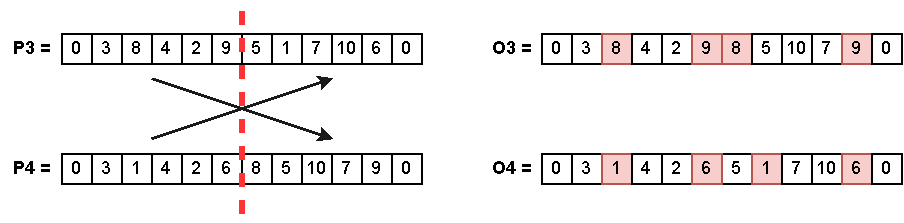
\includegraphics[width=\textwidth]
	{../images/crossover-1b}
	\end{figure}

	I nodi 8, 9, sono visitati 2 volte in O3. \\
	I nodi 1, 6, sono visitati 2 volte in O4.

\framebreak

	I nodi visitati 2 volte possono essere o di pickup o di delivery.

	\textbf{Caso 1: tutti i nodi visitati 2 volte sono delivery (vedi O3)} \\
	Si fa ereditare al figlio, dal secondo genitore, solo la posizione relativa dei nodi e non quella assoluta $\Rightarrow$ nella prima parte del figlio si mantiene la posizione assoluta dei geni del primo genitore, e solo quella relativa dell’altro genitore nella seconda parte. \\
Ruolo asimmetrico dei genitori in ciascun figlio dovuto alla asimmetria nell’ereditare le parti della sequenza (nessun figlio eredita la posizione assoluta nella seconda parte della sequenza di alcun genitore, quell’informazione viene \emph{persa}).

      	\begin{figure}[h]
	\centering
	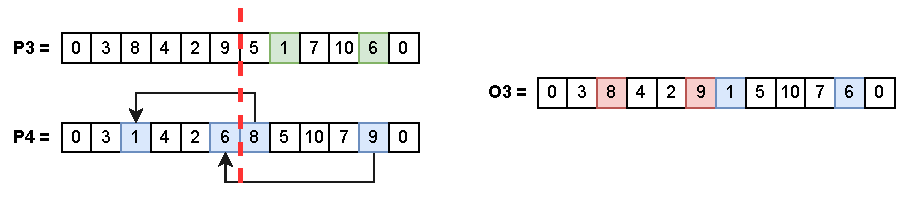
\includegraphics[width=\textwidth]
	{../images/crossover-1c}
	\end{figure}

\framebreak

	\textbf{Caso 2: tutti i nodi visistati 2 volte sono pickup (vedi O2)} \\
	Nella prima parte del figlio si mantiene la posizione assoluta dei geni del primo genitore, nella seconda parte si cancellano i nodi duplicati e si inseriscono i nodi di pickup nella prima parte, rispettando l’ordine relativo.

      	\begin{figure}[h]
	\centering
	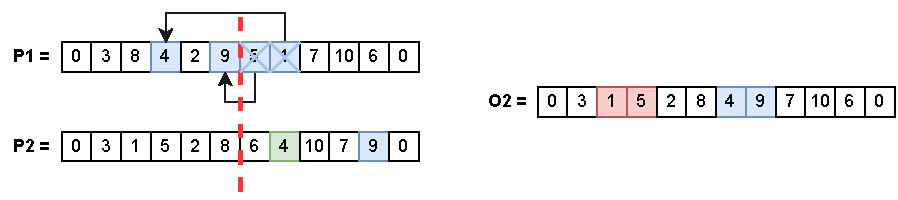
\includegraphics[width=\textwidth]
	{../images/crossover-1d}
	\end{figure}

\framebreak

	\textbf{Caso 3: i nodi visitati 2 volte sono sia pickup che delivery (vedi O1 e O4)} \\
	Tratto i nodi di delivery come il \emph{Caso 1} mentre i nodi di pickup come il \emph{Caso 2}

      	\begin{figure}[h]
	\centering
	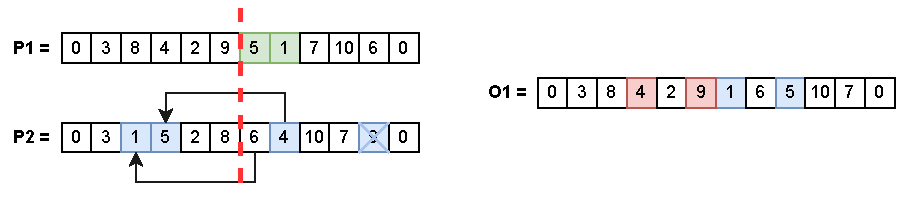
\includegraphics[width=\textwidth]
	{../images/crossover-1e}
	\end{figure}

\framebreak

	\textbf{Performance nel tempo}
      	\begin{figure}[h]
	\centering
	\includegraphics[width=\textwidth]
	{../charts/19 Performance dell'algoritmo Genetic Algorithm}
	\end{figure}

\end{frame}

\subsection{Confronto}
\begin{frame}[allowframebreaks]{\subsecname}

	\textbf{Performance nel tempo}
      	\begin{figure}[h]
	\centering
	\includegraphics[width=\textwidth]
	{../charts/20a Confronto tra algoritmi}
	\end{figure}

\framebreak

	\textbf{Performance costo soluzione}
      	\begin{figure}[h]
	\centering
	\includegraphics[width=\textwidth]
	{../charts/20b Confronto tra algoritmi}
	\end{figure}

\framebreak

	\textbf{Performance errore assoluto}
      	\begin{figure}[h]
	\centering
	\includegraphics[width=\textwidth]
	{../charts/20c Confronto tra algoritmi}
	\end{figure}

\framebreak

	\textbf{Performance errore relativo}
      	\begin{figure}[h]
	\centering
	\includegraphics[width=\textwidth]
	{../charts/20d Confronto tra algoritmi}
	\end{figure}

\end{frame}

\subsection{Conclusioni}
\begin{frame}{\subsecname}

	\begin{itemize}
		\item
		Per istanze del problema piccole (fino $n = 6$) è possibile utilizzare il metodo enumerativo avendo la certezza di trovare un ottimo globale
		\item
		Le procedure euristiche di tipo Greedy, producono velocemente i risultati ma in generale non trovano soluzioni ottimali
		\item
		Si può osservare che nella maggior parte dei casi si è sempre riusciti a migliorare la soluzione iniziale trovata tramite le 3 greedy utilizzando i diversi algoritmi di miglioramento
		\item
		Tra gli algoritmi di miglioramento implementati il più veloce è il Simulated Annealing mentre l'algoritmo che da la miglior soluzione (con le istanze testate) è il Tabu Search
		\item
		In generale non c’è dominanza tra le varie euristiche. Con un tuning accurato è possible migliorare ulteriormente i vari algoritmi sia in termini di soluzioni prodotte per una classe di istanze che in termini di velocità di esecuzione
		\item
		I vari algoritmi restituiscono soluzioni applicabili anche a contesti reali (è possible integrare il codice sviluppato in piattaforme/applicativi reali)
	\end{itemize}

\end{frame}

\begin{frame}{Bibliografia}

	\bibliography{bibliografia.bib}
	\bibliographystyle{abbrv}

\end{frame}

\begin{frame}[standout]
Grazie per l'attenzione
\end{frame}

\end{document}